\chapter{Schemes} \label{chapter: schemes}
    \begin{abstract}
        
    \end{abstract}
    
    \minitoc

    \section{Affine schemes}
        \subsection{The logical approach}
            \subsubsection{The prime spectrum of a commutative ring} \index{$\Spec$}
                \begin{definition}[Spectra of commutative rings]
                    To any commutative ring $R$, let us \textit{contravariantly functorially} associate, first of all, a set $\Spec R$ consisting of all prime ideals of $R$. This is called the spectrum, or the prime spectrum, of $R$. In other words, $\Spec$ is a functor from $\Cring^{\op}$ to $\Sets$.
                \end{definition}
                \begin{remark}[Why is $\Spec$ a contravariant functor ?]
                    One can very well construct the theory of affine schemes based on an alternative \textit{covariant} functor $"\Spec": \Cring \to \Sets$, which assigns to a commutative ring its set of prime ideals too. However, this would not have made our lives easy, as the images under ring homomorphisms of a prime ideal is not necessarily prime, whereas the preimage under ring homomorphisms of a prime ideal is always prime. In particular, this means that requiring $\Spec$ to be a contravariant functor ensures that to-be morphisms between affine schemes would always exist, given that the correpsonding morphism between commutative rings exists. In fact, this also proves that $\Spec$ is a well-defined functor, as it guarantees that each commutative ring homomorphism $f: A \to B$ is sent to a \textit{function} $\Spec f$ that maps each element $\q \in \Spec B$ to a unique element $(\Spec f)(\q)$ of $\Spec A$.
                \end{remark}
                \begin{example}[Some interesting underlying sets of ring spectra] \label{example: spectra_sets}
                    \noindent
                    \begin{enumerate}
                        \item \textbf{(Spectra of fields):} If $k$ is any field, then $\Spec k = \{(0)\}$. To see why this is the case, first of all, let $I$ be an ideal of $k$ that is neither $(0)$ nor $k$. We know that ideals are closed under linear combinations; in this particular instance, $I$ is closed under $k$-linear combinations. Thus, if we view $k$ as a vector space over itself, then $I$ must be a non-zero proper subspace of $k$, since $I$ is a subset of $k$ that is closed under $k$-linear combinations (one could also argue that by the first isomorphism theorem, $I$ is the kernel of some ring homomorphism whose domain is $k$, and we know that kernels are subspaces). Either way, this would mean that:
        					$$0 = \dim_k 0 < \dim_k I < \dim_k k = 1$$
        				and since dimensions of vector spaces are natural numbers, there will be no such natural number $\dim_k I$, i.e. $I$ does not exist. Note that the zero ideal $(0)$ is trivially the zero subspace $0$ of $k$.
        				\item \textbf{(Spectrum of the zero ring):} $\Spec 0 = \varnothing$, because prime ideals are defined to be proper.
        				\item \textbf{(The zero ideal):} The zero ideal is not necessarily prime; as a matter of fact, it is only so inside an integral domain. When zero-divisors are present, say in $\Z/n\Z$ with $n$ composite, the statement:
        				    $$xy \in (0)$$
    				    might not imply that $x = y = 0$, but instead, that $x \in (p)$ and $y \in (q)$, with $p, q$ integers such that $pq = n$.
        				\item \textbf{(The complex affine line):} Due to the algebraic closure of $\bbC$, the points of the complex affine line $\A^1_{\bbC} := \Spec \bbC[x]$ (with $t$ some formal variable) are prime ideals of the form $(x - a)$ wherein $a \in \bbC$, along with the prime ideal $(0)$. To see in more details why this is the case, let us first recall because $\bbC$ is a separably closed field, every single-variable polynomial over $\bbC$ splits completely into linear factor. This, along with the fact that $\bbC[x]$ is a PID, tells us that ideals of $\bbC[x]$ are actually all contained in \textit{principal} ideals generated by linear polynomials; note that these principal ideals are prime, precisely because $\bbC$ is separably closed. Lastly. because $\bbC$ is algebraically closed, there is a bijective correspondence between the principal ideals generated by linear polyonomials $(x - a)$ and the individual complex numbers $a \in \bbC$. Thus, the prime ideals of $\bbC[x]$ are either of the form $(0)$ or $(x - a)$, wherein $a \in \bbC$. 
        				\\
        				Below is an illustration by Ravi Vakil of the complex affine line:
        				    \begin{figure}[H]
        				        \centering
        				        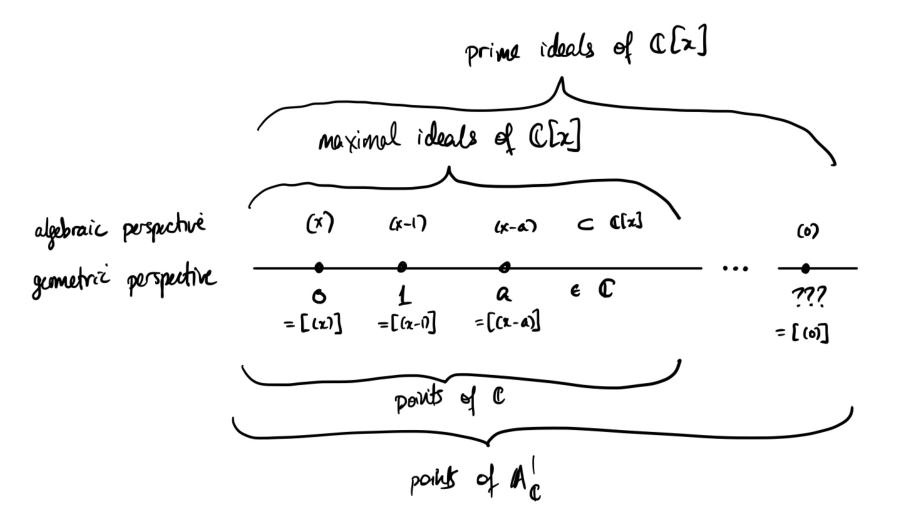
\includegraphics[width=\linewidth,height=\textheight,keepaspectratio]{Figures/complex affine line.png}
        				        \caption{The complex affine line $\A^1_{\bbC}$ (\cite{risingsea}, figure 3.1)}
        				        \label{fig: complex_affine_line}
        				    \end{figure}
        				This result generalises in an obvious manner to algebraically closed fields other than $\bbC$; so for instance, studying schemes over the field $\overline{\Q}$ of algebraic numbers might help one understand more about polynomials with rational coefficients.
        				\item \textbf{(The affine line over a separably closed but not algebraically closed field):} Let $k$ be a field that is separably closed but not algebraically closed (we can take $k = \F_p(t)^{\sep}$, for example). Then, the set of non-zero prime ideals of $\A^1_k$ need not be in bijection with $k$ itself.
        				\item \textbf{(Spectrum of the integers):} The prime ideals of $\Z$ are either generated by prime numbers themselves, or the zero ideal $(0)$. Thus, the set $\Spec \Z$ is in bijection with the \textit{union} of the set of all prime numbers and the set $\{(0)\}$. 
                    \end{enumerate}
                \end{example}
            
            \subsubsection{The Zariski topology} \index{Topology!Zariski}
                \begin{definition}[Zariski-closed subsets] \label{def: zariski_closed}
                    Let $R$ be a commutative ring and let $\calF$ be an arbitrary subset of $R$. Then, let us declare that sets of the following form are closed in the to-be Zariski topology:
                        $$V(\calF) := \left\{\p \in \Spec R \mid \p \supset \calF \right\}$$
                    When it might be possible to confuse Zariski-closed subsets of different ring spectra, we will write $V_R(\calF)$ instead of simply $V(\calF)$.
                \end{definition}
                \begin{remark}
                    Of course, sets of the form $\Spec R \setminus V(\calF)$ are Zariski-open (that is, if we are assuming that the \href{https://ncatlab.org/nlab/show/excluded+middle}{\underline{the Law of Excluded Middle}} holds).
                \end{remark}
                
                \begin{proposition}[Well-definiteness of the Zariski topology] \label{prop: zariski_closed_well_definiteness}
                    Let $R$ be an arbitrary commutative ring and assume the Law of Excluded Middle. Then, Zariski-closed subsets as defined in \ref{def: zariski_closed} actually define a topology on $\Spec R$, which of course, is called the Zariski topology.
                \end{proposition}
                    \begin{proof}
                        For each subset $\calF$ of $R$, let us write $I(\calF)$ for the $R$-ideal generated by $\calF$. Let us now verify the axioms defining topologies on sets one-by-one.
                            \begin{enumerate}
                                \item \textbf{(The empty set and the whole set are closed):} The empty set is just $V(R)$ and that $\Spec R$ is just $V\left((0)\right)$, which are, by definition, closed in the Zariski topology. Thus, both the empty set and the whole space are Zariski-closed.
                                \item \textbf{(Finite unions of closed sets are closed):} Let $\{V(\calF_{\alpha})\}_{\alpha \in A}$ be a \textit{finite} set of Zariski-closed subsets of $\Spec R$ and consider the following chain of logical \textit{implications} (wherein $\p$ is a prime ideal of $R$, even though this fact can be inferred from the statements themselves):
                                    $$
                                        \begin{aligned}
                                            & \p \in \bigcup_{\alpha \in A} V(\calF_{\alpha})
                                            \\
                                            \iff & \exists \alpha \in A: \p \in V(\calF_{\alpha})
                                            \\
                                            \iff & \exists \alpha \in A: \p \supset \calF_{\alpha}
                                            \\
                                            \iff & \bigvee_{\alpha \in A} (\p \supset \calF_{\alpha})
                                            \\
                                            \implies & \forall \left(f_{\alpha}\right)_{\alpha \in A} \in \prod_{\alpha \in A} \calF_{\alpha}: \prod_{\alpha \in A} f_{\alpha} \in \p
                                            \\
                                            \iff & \bigwedge_{\left(f_{\alpha}\right)_{\alpha \in A} \in \prod_{\alpha \in A} \calF_{\alpha}} \left(\prod_{\alpha \in A} f_{\alpha} \in \p\right)
                                            \\
                                            \iff & \p \supset \left\{\prod_{\alpha \in A} f_{\alpha} \: \bigg| \: \forall \alpha \in A: f_{\alpha} \in \calF_{\alpha} \right\}
                                            \\
                                            \iff & \p \in V\left(\left\{\prod_{\alpha \in A} f_{\alpha} \: \bigg| \: \forall \alpha \in A: f_{\alpha} \in \calF_{\alpha} \right\}\right)
                                        \end{aligned}
                                    $$
                                wherein the fourth line, in particular, holds due to the fact that ideals, by definition, are closed under scalar multiplication by elements of their ambient rings. Now, to upgrade the fourth line to an equivalence, we can show that:
                                    $$\bigwedge_{\left(f_{\alpha}\right)_{\alpha \in A} \in \prod_{\alpha \in A} \calF_{\alpha}} \left(\prod_{\alpha \in A} f_{\alpha} \in \p\right) \implies \bigvee_{\alpha \in A} (\p \supset \calF_{\alpha})$$
                                or, as we have assumed that the Law of Excluded Middle holds, we have the following:
                                    $$
                                        \begin{aligned}
                                            & \left(\bigwedge_{\left(f_{\alpha}\right)_{\alpha \in A} \in \prod_{\alpha \in A} \calF_{\alpha}} \left(\prod_{\alpha \in A} f_{\alpha} \in \p\right) \implies \bigvee_{\alpha \in A} (\p \supset \calF_{\alpha})\right)
                                            \\
                                            \vdash & \left(\neg \bigwedge_{\left(f_{\alpha}\right)_{\alpha \in A} \in \prod_{\alpha \in A} \calF_{\alpha}} \left(\prod_{\alpha \in A} f_{\alpha} \in \p\right) \implies  \neg \bigvee_{\alpha \in A} (\p \supset \calF_{\alpha})\right)
                                        \end{aligned}
                                    $$
                                meaning that we can prove the contraposition instead. To that end, consider the following:
                                    $$
                                        \begin{aligned}
                                            & \neg \bigwedge_{\left(f_{\alpha}\right)_{\alpha \in A} \in \prod_{\alpha \in A} \calF_{\alpha}} \left(\p \ni \prod_{\alpha \in A} f_{\alpha}\right)
                                            \\
                                            \implies & \bigvee_{\left(f_{\alpha}\right)_{\alpha \in A} \in \prod_{\alpha \in A} \calF_{\alpha}} \neg \left(\p \ni \prod_{\alpha \in A} f_{\alpha}\right)
                                            \\
                                            \implies & \bigwedge_{\alpha \in A} \left(\bigvee_{f_{\alpha} \in \calF_{\alpha}} \neg(\p \ni f_{\alpha})\right)
                                            \\
                                            \implies & \bigwedge_{\alpha \in A} \left(\neg \bigwedge_{f_{\alpha} \in \calF_{\alpha}} (\p \ni f_{\alpha})\right)
                                            \\
                                            \implies & \bigwedge_{\alpha \in A} \neg (\p \supset \calF_{\alpha})
                                            \\
                                            \implies & \neg \bigvee_{\alpha \in A} (\p \supset \calF_{\alpha})
                                        \end{aligned}
                                    $$
                                Thus, we have managed to show that:
                                    $$\neg \bigwedge_{\left(f_{\alpha}\right)_{\alpha \in A} \in \prod_{\alpha \in A} \calF_{\alpha}} \left(\prod_{\alpha \in A} f_{\alpha} \in \p\right) \implies  \neg \bigvee_{\alpha \in A} (\p \supset \calF_{\alpha})$$
                                and therefore:
                                    $$\p \in \bigcup_{\alpha \in A} V(\calF_{\alpha}) \iff \p \in V\left(\left\{\prod_{\alpha \in A} f_{\alpha} \: \bigg| \: \forall \alpha \in A: f_{\alpha} \in \calF_{\alpha} \right\}\right)$$
                                Because $\p$ was chosen arbitrarily, this implies that:
                                    $$\bigcup_{\alpha \in A} V(\calF_{\alpha}) = V\left(\left\{\prod_{\alpha \in A} f_{\alpha} \: \bigg| \: \forall \alpha \in A: f_{\alpha} \in \calF_{\alpha} \right\}\right)$$
                                Hence, the \textit{finite} union $\bigcup_{\alpha \in A} V(\calF_{\alpha})$ is Zariski-closed by definition, and consequently, all finite unions of Zariski-closed sets are closed in the Zariski topology themselves (since $\{\calF_{\alpha}\}_{\alpha \in A}$ is an arbitrary fintie set of subsets of $R$). Note that the finiteness assumption on the index set $A$ is crucial, as without it, one would not be able to properly make sense of the product $\prod_{\alpha \in A} f_{\alpha}$.
                                \item \textbf{(Intersections of closed sets are closed):} Let $\{V(\calF_{\alpha})\}_{\alpha \in A}$ be an \textit{arbitrary} set of Zariski-closed subsets of $\Spec R$ and consider the following chain of logical equivalences (wherein $\p$ is a prime ideal of $R$, and again, this fact can be deduced from the statements themselves):
                                    $$
                                        \begin{aligned}
                                            & \p \in \bigcap_{\alpha \in A} V(\calF_{\alpha})
                                            \\
                                            \iff & \forall \alpha \in A: \p \in V(\calF_{\alpha})
                                            \\
                                            \iff & \forall \alpha \in A: \p \supset \calF_{\alpha}
                                            \\
                                            \iff & \p \supset I\left(\bigcup_{\alpha \in A} \calF_{\alpha}\right)
                                            \\
                                            \iff & \p \in V\left(I\left(\bigcup_{\alpha \in A} \calF_{\alpha}\right)\right)
                                        \end{aligned}
                                    $$
                                It tells us that \textit{any} prime ideal $\p$ is in an intersection of Zariski-closed subsets of $\Spec R$ defined by subsets $\calF_{\alpha}$ of $R$ if and only if it is in the Zariski-closed subset of $\Spec R$ defined by the ideal generated by the union of the sets $\calF_{\alpha}$, or in other words, that:
                                    $$\bigcap_{\alpha \in A} V(\calF_{\alpha}) = V\left(I\left(\bigcup_{\alpha \in A} \calF_{\alpha}\right)\right)$$
                                In turn, this implies that the intersection of the Zariski-closed sets $V(\calF_{\alpha})$ is itself closed in the Zariski topology, and since the index set $A$ is was chosen arbitrarily, this means that arbitrary intersections of Zariski-closed sets are themselves Zariski-closed.
                            \end{enumerate}
                        Thus, with closed sets as in definition \ref{def: zariski_closed}, the Zariski topology on prime spectra of commutative rings is well-defined.
                    \end{proof}
                \begin{corollary}[Quotients are closed] \label{coro: quotients_are_closed}
                    Let $R$ be a commutative ring and let $I$ be an $R$-ideal. Then, $\Spec R/I$ is homeomorphic to a Zariski-closed subset of $\Spec R$. 
                \end{corollary}
                    \begin{proof}
                        This comes from a straightforward application of the third isomorphism theorem for modules.
                    \end{proof}
                    
                \begin{definition}[A different approach: Zariski-open sets] \label{def: zariski_open}
                    Let $R$ be a commutative ring. Then, let us declare that subsets of $\Spec R$ of the following form are open in the to-be Zariski topology:
                        $$D(f) := \{\p \in \Spec R \mid \p \not \ni f\}$$
                    Whenever referring to more than one ring spectra, it might be beneficial to specifically write $D_R(f)$ instead of $D(f)$.
                \end{definition}
                \begin{remark} \label{remark: basic_opens_complements}
                    For any commutative ring $R$, one can show through the following logical equivalences that:
                        $$D(f) = \Spec R \setminus V\left((f)\right)$$
                    wherein $\p$ is an arbitrary prime ideal of $R$:
                        $$
                            \begin{aligned}
                                & \p \in D(f)
                                \\
                                \iff & \p \in \{\q \in \Spec R \mid \q \not \ni f\}
                                \\
                                \iff & \neg(\p \ni f)
                                \\
                                \iff & \neg(\p \supset (f))
                                \\
                                \iff & \p \in \Spec R \setminus \{\q \in \Spec R \mid \q \supset (f)\}
                                \\
                                \iff & \p \in \Spec R \setminus V\left((f)\right)
                            \end{aligned}
                        $$
                \end{remark}
                
                \begin{proposition}[Well-definiteness of the Zariski topology] \label{prop: zariski_open_well_definiteness}
                    Let $R$ be an arbitrary commutative ring and assume the Law of Excluded Middle. Then, Zariski-open subsets as defined in \ref{def: zariski_open} actually define a topology on $\Spec R$, which of course, is called the Zariski topology.
                \end{proposition}
                    \begin{proof}
                        Let us verify the axioms defining topologies on sets one-by-one.
                            \begin{enumerate}
                                \item \textbf{(The empty set and the whole set are open):} Consider the set $D(1)$, which by definition, is given by:
                                    $$D(1) := \{\p \in \Spec R \mid \p \not \ni 1\}$$
                                Because prime ideals are defined to be proper, and because proper ideals are never (multiplicatively) unital, one gets that:
                                    $$D(1) = \Spec R$$
                                In other words, the whole of $\Spec R$ is open by definition. Now, consider the following:
                                    $$D(0) := \{\p \in \Spec R \mid \p \not \ni 0\} = \varnothing$$
                                which holds because ideals are submodules of their ambient rings, and modules over rings must contain $0$ (as an additive identity) by definition. Thus, the empty set is also Zariski-open by definition. 
                                \item \textbf{(Unions of open sets are open):} Let $\{f_{\alpha}\}_{\alpha \in A}$ be an \textit{arbitrary} set of elements of $R$ and let us apply remark \ref{remark: basic_opens_complements} to get the following chain of logical equivalences regarding the union of the sets $D(f_{\alpha})$, wherein $\p$ is an \textit{arbitrary} prime ideal of $R$:
                                    $$
                                        \begin{aligned}
                                            & \p \in \bigcup_{\alpha \in A} D(f_{\alpha})
                                            \\
                                            \iff & \bigvee_{\alpha \in A} \left(\p \in D(f_{\alpha})\right)
                                            \\
                                            \iff & \bigvee_{\alpha \in A} \neg \left(\p \in V\left((f_{\alpha})\right)\right)
                                            \\
                                            \iff & \neg \bigwedge_{\alpha \in A} \left(\p \in V\left((f_{\alpha})\right)\right)
                                            \\
                                            \iff & \p \in \Spec R \setminus \bigcap_{\alpha \in A} V\left((f_{\alpha})\right)
                                        \end{aligned}
                                    $$
                                This shows that:
                                    $$\bigcup_{\alpha \in A} D(f_{\alpha}) = \Spec R \setminus \bigcap_{\alpha \in A} V\left((f_{\alpha})\right)$$
                                In proposition \ref{prop: zariski_closed_well_definiteness}, we have already shown using only definition \ref{def: zariski_closed} that arbitrary intersections of Zariski-closed sets are Zariski-closed themselves; in particular, this means that $\bigcap_{\alpha \in A} V\left((f_{\alpha})\right)$ is Zariski-closed. Then, by using the Law of Excluded Middle, one can see that the complement $\Spec R \setminus \bigcap_{\alpha \in A} V\left((f_{\alpha})\right)$ is necessarily Zariski-open. Thus, arbitrary unions of Zariski-open sets are Zariski-open themselves.
                                \item \textbf{(Finite intersections of open sets are open):} Let $\{f_{\alpha}\}_{\alpha \in A}$ be an \textit{finite} set of elements of $R$ and consider the following chain of logical equivalences regarding the union of the sets $D(f_{\alpha})$, wherein $\p$ is a prime ideal of $R$:
                                    $$
                                        \begin{aligned}
                                            & \neg \left(\p \in \bigcap_{\alpha \in A} D(f_{\alpha})\right)
                                            \\
                                            \iff & \neg \bigwedge_{\alpha \in A} \left(\p \in D(f_{\alpha})\right)
                                            \\
                                            \iff & \bigvee_{\alpha \in A} \neg \left(\p \in D(f_{\alpha})\right)
                                            \\
                                            \iff & \bigvee_{\alpha \in A} \left(\p \in \Spec R \setminus D(f_{\alpha})\right)
                                            \\
                                            \iff & \bigvee_{\alpha \in A} \left(\p \in V\left((f_{\alpha})\right)\right)
                                            \\
                                            \iff & \p \in \bigcup_{\alpha \in A} V\left((f_{\alpha})\right)
                                        \end{aligned}
                                    $$
                                (let us note that the fifth line holds thanks to remark \ref{remark: basic_opens_complements}). Now, the contraposition of the equivalence:
                                    $$\neg \left(\p \in \bigcap_{\alpha \in A} D(f_{\alpha})\right) \iff \p \in \bigcup_{\alpha \in A} V\left((f_{\alpha})\right)$$
                                is:
                                    $$\neg \neg \left(\p \in \bigcap_{\alpha \in A} D(f_{\alpha})\right) \iff \neg \left(\p \in \bigcup_{\alpha \in A} V\left((f_{\alpha})\right) \right)$$
                                From this, one gets the following proof:
                                    $$
                                        \begin{aligned}
                                            & \neg \neg \left(\p \in \bigcap_{\alpha \in A} D(f_{\alpha})\right) \iff \neg \left(\p \in \bigcup_{\alpha \in A} V\left((f_{\alpha})\right) \right)
                                            \\
                                            \vdash & \left(\p \in \bigcap_{\alpha \in A} D(f_{\alpha})\right) \iff \left(\p \in \Spec R \setminus \bigcup_{\alpha \in A} V\left((f_{\alpha})\right) \right) 
                                            \\
                                            \vdash & \left(\bigcap_{\alpha \in A} D(f_{\alpha}) = \Spec R \setminus \bigcup_{\alpha \in A} V\left((f_{\alpha})\right)\right)
                                        \end{aligned}
                                    $$
                                Lastly, let us recall that by \ref{prop: zariski_closed_well_definiteness}, the \textit{finite} union $\bigcup_{\alpha \in A} V\left((f_{\alpha})\right)$ of Zariski-closed sets is Zariski-closed itself, meaning that by the Law of Excluded Middle, the complement $\Spec R \setminus \bigcup_{\alpha \in A} V\left((f_{\alpha})\right)$ must be Zariski-open. Thus, the union $\bigcap_{\alpha \in A} D(f_{\alpha})$ is Zariski-open. Note that the finiteness assumption on the index set $A$ is crucial, as otherwise, the union $\bigcup_{\alpha \in A} V\left((f_{\alpha})\right)$ might not be Zariski-closed.
                            \end{enumerate}
                        Thus, with open sets as in definition \ref{def: zariski_open}, the Zariski topology on prime spectra of commutative rings is well-defined.
                    \end{proof}
                
                \begin{proposition}[Unifying the two definitions] \label{prop: zariski_topology_equivalence}
                    By asuming the Law of Excluded Middle, one gets the same topology on spectra of commutative rings via the approaches presented in definitions \ref{def: zariski_closed} and \ref{def: zariski_open}.
                \end{proposition}
                    \begin{proof}
                        Let $R$ be a commutative ring. It is sufficient to show that for each element $f \in R$, the complement $\Spec R \setminus D(f)$ is closed in the sense of definition \ref{def: zariski_closed}, or equivalently, for each subset $\calF \subset R$, the complement $\Spec R \setminus V(\calF)$ is open in the sense of definition \ref{def: zariski_open}. We will be attempting the second approach. To that end, let us directly the following chain of logical equivalences:
                            $$
                                \begin{aligned}
                                    & \p \in \bigcup_{\alpha \in A} D(f_{\alpha})
                                    \\
                                    \iff & \exists \alpha \in A: \p \in D(f_{\alpha})
                                    \\
                                    \iff & \exists \alpha \in A: \p \in \{\q \in \Spec R \mid \q \not \ni f_{\alpha}\}
                                    \\
                                    \iff & \exists \alpha \in A: \p \not \ni f_{\alpha}
                                    \\
                                    \iff & \bigvee_{\alpha \in A} \neg\left(\p \ni f_{\alpha}\right)
                                    \\
                                    \iff & \neg \bigwedge_{\alpha \in A} (\p \ni f_{\alpha}) 
                                    \\
                                    \iff & \neg \left(\p \supset \bigcup_{\alpha \in A} \{f_{\alpha}\}\right)
                                    \\
                                    \iff & \neg \left(\p \supset \{f_{\alpha}\}_{\alpha \in A}\right)
                                    \\
                                    \iff & \p \in \Spec R \setminus \left\{\q \in \Spec R \mid \q \supset \{f_{\alpha}\}_{\alpha \in A}\right\}
                                    \\
                                    \iff & \p \in \Spec R \setminus V\left(\{f_{\alpha}\}_{\alpha \in A}\right)
                                \end{aligned}
                            $$
                        Thus:
                            $$\bigcup_{\alpha \in A} D(f_{\alpha}) = \Spec R \setminus V\left(\{f_{\alpha}\}_{\alpha \in A}\right)$$
                        i.e. the complement of the Zariski-closed set $V\left(\{f_{\alpha}\}_{\alpha \in A}\right)$ inside $\Spec R$ is a union of Zariski-open sets $D(f_{\alpha})$, which we know from proposition \ref{prop: zariski_open_well_definiteness} to be Zariski-open itself. As stated, this implies that definitions \ref{def: zariski_closed} and \ref{def: zariski_open} give us the same Zariski topology on prime spectra of commutative rings.
                    \end{proof}
                \begin{corollary} \label{coro: zariski_basis}
                    Let $R$ be a commutative ring and let $f$ denote elements of $R$. Then, the distinguished Zariski-open sets $D(f)$ form a base of the Zariski topology on $\Spec R$.
                \end{corollary}
                    \begin{proof}
                        This is a direct consequence of the fact that complements of Zariski-closed sets are unions of Zariski-open sets of the form $D(f)$.
                    \end{proof}
                
                We have managed to show that on each ring spectrum, there is a canonical topology, namely the Zariski topology. A naturaly follow-up question is thus: can we upgrade $\Spec$ to a functor whose domain is $\Top$ instead of $\Sets$ ? Luckily, the answer is yes, although we will need to do some work to show that this is the case. 
                \begin{proposition}[Continuous functions between spectra] \label{prop: continuous_functions_between_spectra}
                    By equipping prime spectra of commutative rings with the Zariski topology (in either the sense of definition \ref{def: zariski_closed} or \ref{def: zariski_open}), one naturally gets a functor:
                        $$\Spec: \Cring^{\op} \to \Top$$
                    assigning to commutative rings their respective Zariski topological spaces.
                \end{proposition}
                    \begin{proof}
                        It will suffice to show that given any ring homomorphism $f: A \to B$, the induced map $\Spec f: \Spec B \to \Spec A$ is continuous, which we can do by showing that preimages of Zariski-open subsets of $\Spec A$ under $\Spec f$ are closed in $\Spec B$; in fact, we can restrict our attention to \textit{basic} open subsets of $\Spec A$ (i.e. subsets of the form $D_A(a)$, for some $a \in A$), as they form a basis for the Zariski topology on $\Spec A$. Let $D_A(a)$ be such a basic open set. It preimage under $\Spec f$ is thus the following subset of $\Spec B$:
                            $$(\Spec f)^{-1}\left(D_A(a)\right) = \{\q \in \Spec B \mid (\Spec f)(\q) \in D_A(a)\}$$
                        Writing out the definition of $D_A(a)$ (cf. definition \ref{def: zariski_open}) then gives the following chain of logical equivalences:
                            $$
                                \begin{aligned}
                                    & \q \in (\Spec f)^{-1}\left(D_A(a)\right)
                                    \\
                                    \iff & (\Spec f)(\q) \in D_A(a)
                                    \\
                                    \iff & f^{-1}(\q) \in D_A(a)
                                    \\
                                    \iff & \neg(f^{-1}(\q) \ni a)
                                    \\
                                    \iff & \neg(\q \ni f(a))
                                    \\
                                    \iff & \q \in D_B(f(a))
                                \end{aligned}
                            $$
                        which proves that:
                            $$(\Spec f)^{-1}\left(D_A(a)\right) = D_B(f(a))$$
                        and because $D_B(f(a))$ is open by definition, so is the preimage $(\Spec f)^{-1}(D_A(a))$. As stated at the beginning, this implies that $\Spec f$ is a continuous function, and thus there exists a functor:
                            $$\Spec: \Cring^{\op} \to \Top$$
                        assigning commutative rings and homomorphisms between them to ring spectra equipped with the Zariski topology and continuous maps in between.
                    \end{proof}
                    
                \begin{example}[Topologically interesting ring spectra]
                    \noindent
                    \begin{enumerate}
                        \item \textbf{(The complex affine plane and complex affine $n$-spaces):}
                            \begin{figure}[H]
                                \centering
                                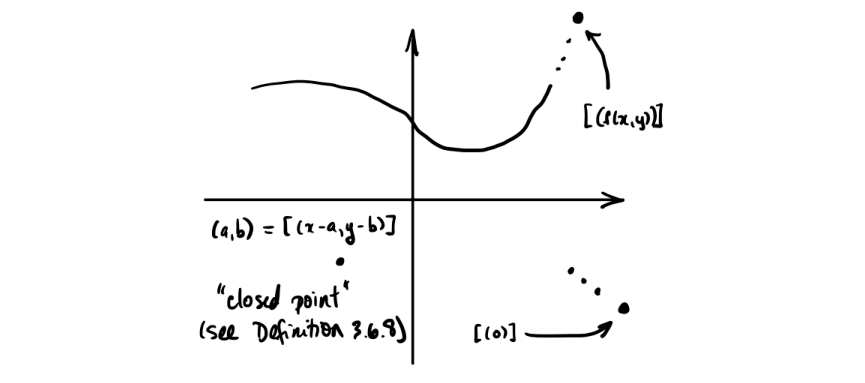
\includegraphics[width=\linewidth,height=\textheight,keepaspectratio]{Figures/complex affine plane.png}
                                \caption{The complex affine plane $\A^2_{\bbC}$ (\cite{risingsea}, figure 3.3)}
                                \label{fig: complex_affine_plane}
                            \end{figure}
                        \item \textbf{(Revisiting $\Spec \Z$):}
                            \begin{figure}[H]
                                \centering
                                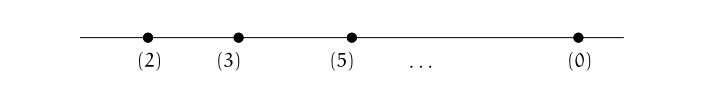
\includegraphics[width=\linewidth,height=\textheight,keepaspectratio]{Figures/Spec Z.png}
                                \caption{$\Spec \Z$ (\cite{risingsea}, figure 3.2)}
                                \label{fig: Spec_Z}
                            \end{figure}
                        \item \textbf{(A conic):}
                            \begin{figure}[H]
                                \centering
                                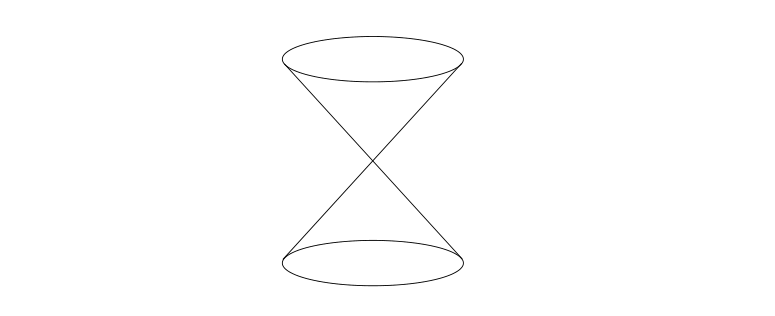
\includegraphics[width=\linewidth,height=\textheight,keepaspectratio]{Figures/conic.png}
                                \caption{A conic which is Zariski-closed inside $\A^3_{\bbC}$ (\cite{risingsea}, figure 3.4)}
                                \label{fig: conic}
                            \end{figure}
                    \end{enumerate}
                \end{example}
                
                \begin{remark}[Comparing $\Spec$ and $\Spm$]
                    \noindent
                    \begin{enumerate}
                        \item \textbf{(Why maximal ideals ?):} Historically (and only because mathematicians were more interested in complex algebraic geometry back in the days), it was not the set of prime ideals of a commutative ring that was considered, but rather, the set of \textit{maximal} ideals. This was not out of \textit{na\"ivet\'e}, though. Maximal ideals enjoy being closed points in prime spectra of commutative rings (one can prove this by first looking at varieties $V(\m)$ associated to maximal ideals $\m$ of some commutative ring $R$, and then applying the definition of the (underlying set of) these varieties as spaces whose points are prime ideals containing $\m$, and then lastly, applying the usual definition of topological closures; as a corollary, one gets that prime ideals that are not maximal get sent by $\Spec$ to non-closed points in $\Spec R$), and so doing geometry with them is a lot more intuitive (albeit more restrictive as well) then doing so with all prime ideals. For instance, the underlying set of $\Spm \bbC[x]$ is precisely $\bbC$, whereas that of $\Spec \bbC[x]$ can be thought of as $\bbC \cup \{\infty\}$, i.e. as the Riemann sphere; in particular, the zero ideal $(0)$ corresponds to the point at infinity $\infty$. 
                        \item \textbf{(On GAGA theorems):} 
                    \end{enumerate}
                \end{remark}
                
                \begin{example}[Non-isomorphic rings with homeomorphic spectra] \label{example: nonisomorphic_rings_with_the_same_spectra}
                    The following examples are of non-isomorphic rings with homeomorphic prime spectra; through them, we are able to show that the functor $\Spec: \Cring^{\op} \to \Top$ is not an equivalence of categories (nor even a fully faithful inclusion). 
                    \begin{enumerate}
                        \item \textbf{(Fields):} The prime spectra of any field is just the one-point space, but clearly, not all fields are isomorphic.
                        \item \textbf{(Discrete valuation rings):} The spectrum of any \href{https://en.wikipedia.org/wiki/Discrete_valuation_ring}{\underline{discrete valuation ring}} is homeomorphic to the \href{https://ncatlab.org/nlab/show/Sierpinski+space}{\underline{Sierpi\'nski space}} (to see why this is the case, firstly check that discrete valuation rings only have two prime ideals, one being the zero ideal and one being the unique maximal ideal, and that the latter is a closed point in the spectrum whereas the former is generic), but of course, not all discrete valuation rings are isomorphic to one another.
                    \end{enumerate}
                \end{example}
                
            \subsubsection{How locales are radicalising our ideals} \index{Locales of radical ideals}
                \begin{remark}[The horror of Zariski-open sets]
                    While definition \ref{def: zariski_open} seems on the surface to be a perfectly good notion of open sets in the Zariski topology of commutative ring spectra (see proposition \ref{prop: zariski_open_well_definiteness} for a proof), it is highly unintuitive, in the sense that it is very hard to immediately see that the sets $D(f)$ should indeed be open, and even less so, that they might have anything to do with roots of polynomials. Even more alarmingly, the Zariski topology is somehow a \say{wrong} topology to put on schemes: for instance, Zariski cohomology gives nonsensical results such as:
                        $$\forall i > 0: H_{\Zar}^i(X, \underline{A}) = 0$$
                    for all irreducible schemes $X$ and all local systems $\underline{A}$ (more on this when we discuss \'etale cohomology of schemes). Thus, let us try to refine the definition into something a bit more intuitive, and we will do this via showing that prime spectra are actually \href{https://ncatlab.org/nlab/show/locale}{\underline{locales}} whose \href{https://ncatlab.org/nlab/show/frame}{\underline{frames}} are given by radical ideals. Before that, however, let us recall the definition of the radical of a given ideal as a reminder for readers who might not remember the notion too clearly. 
                \end{remark}
                
                \begin{definition}[Radicals of ideals] \label{def: radicals}
                    \noindent
                    \begin{enumerate}
                        \item \textbf{(The radical of an ideal):} Let $I$ be an ideal of a commutative ring $R$. Then, its radical, denoted by $\sqrt{I}$, is the set given by:
                            $$\sqrt{I} := \{f \in R \mid \exists n \in \N: f^n \in I\}$$
                        \item \textbf{(Radical ideals):} An ideal $\r$ is radical if and only if $\r = \sqrt{\r}$. 
                    \end{enumerate}
                \end{definition}
                \begin{proposition}[Basic properties of radicals] \label{prop: radical_properties}
                    The following are easy to verify properties that radicals possess:
                        \begin{enumerate}
                            \item The radical of an ideal is also an ideal.
                            \item Let $I$ be any ideal of a given commutative ring $R$. Then $\sqrt{I} = \sqrt{\sqrt{I}}$; in other words, radicalisation is idempotent.
                            \item Let $I$ be an ideal of a commutative ring $R$. Then $\sqrt{I^n} = \sqrt{I}$ for all natural numbers $n$. 
                            \item Let $\{I_n\}_{1 \leq n \leq N}$ be a finite set of ideals of a commutative ring $R$. Then $\bigcap_{n = 1}^N \sqrt{I_n} = \sqrt{\bigcap_{n = 1}^N I_n}$. 
                            \item The underlying set of the radical of an ideal $I$ of a commutative ring $R$ is equal to the intersection of all prime ideals of $R$ that (improperly) contain $I$. Consequently, prime ideals are trivially radical.
                            \item  Let $I$ be an ideal of a commutative ring $R$. Then $\sqrt{I} \supseteq I$; in fact, $\sqrt{I}$ is the minimal ideal that contains $I$. 
                            \item An ideal $\r$ of a commutative ring $R$ is radical if and only if the quotient $R/\r$ is reduced.
                \end{enumerate}
                \end{proposition}
                    \begin{proof}
                        As stated, these properties are rather trivial. However, let us nevertheless prove that radicalisation preserves finite intersection, and that the radical of an ideal is the intersection of all prime ideals containing it, as these properties has interesting topological interpretations.
                            \begin{enumerate}
                                \item 
                                    \begin{enumerate}
                                        \item Let $\Nil(R)$ be the nilradical of a commutative ring $R$, which by definition, is the ideal consisting of nilpotent elements of $R$. First of all, note that $\Nil(R)$ is radical, since:
                                            $$\forall x \in \Nil(R): \exists N_x \in \N: n \geq N_x \implies x^n = 0$$
                                        and consequently:
                                            $$\forall x \in \Nil(R): \exists N_x \in \N: x^{N_x} = 0 \in \Nil(R)$$
                                        Furthermore, because sufficiently large powers of nilpotent elements are zero, we have:
                                            $$\Nil(R) = \sqrt{(0)}$$
                                        Let us now try to show that $\Nil(R)$ is the intersection of all prime ideals of $R$, which we note to all trivially contain the zero ideal $(0)$; before we do, however, let us direct the readers' attention to the following fact:
                                            $$\Nil(R) = \bigcap_{\p \in \Spec R} \p \iff \bigwedge_{\p \in \Spec R} \left(\p \supset \Nil(R)\right)$$
                                        which tells us that we can show that $\Nil(R)$ is the intersection of all prime ideals of $R$ via showing that there exists a prime ideal $\p$ of $R$ which does not contain any non-nilpotent element $x \in R$, as we have the following chain of logical equivalences hold:
                                            $$
                                                \begin{aligned}
                                                    & \text{$x$ is \textit{not} nilpotent}
                                                    \\
                                                    \iff & \neg \left(x \in \Nil(R)\right)
                                                    \\
                                                    \iff & \neg \bigwedge_{\p \in \Spec R} \left(\p \ni x\right)
                                                    \\
                                                    \iff & \bigvee_{\p \in \Spec R} \neg \left(\p \ni x\right)
                                                    \\
                                                    \iff & \exists \p \in \Spec R: \neg(\p \ni x)
                                                    \\
                                                    \iff & \exists \p \in D_R(x)
                                                    \\
                                                    \iff & \neg(\Spec R_x = \varnothing)
                                                    \\
                                                    \iff & \neg(R_x = 0)
                                                \end{aligned}
                                            $$
                                        But we know the last line to be true (cf. example \ref{example: reducedeness_and_nilpotency}), so by the arbitrarity of the choice of our non-nilpotent element $x$, there indeed exists a prime $\p$ of $R$ which does not contain any non-nilpotent element, which as stated, implies that:
                                            $$\Nil(R) = \bigcap_{\p \in \Spec R} \p$$
                                        \item Now, let us apply what we have just shown to the ring $R/I$, with $I$ an arbitrary ideal of $R$: in particular, we get the following result:
                                            $$\Nil(R/I) = \bigcap_{\p \in \Spec R/I} \p = \bigcap_{\p \in V_R(I)} \p$$
                                        Lastly, note that:
                                            $$
                                                \begin{aligned}
                                                    \Nil(R/I) & = \{x \in R \mid \exists n \in \N: x^n = 0_{R/I}\}
                                                    \\
                                                    & = \{x \in R \mid \exists n \in \N: x^n \in I\}
                                                    \\
                                                    & = \sqrt{I}
                                                \end{aligned}
                                            $$
                                        and so:
                                            $$\sqrt{I} = \bigcap_{\p \in V_R(I)} \p$$
                                    \end{enumerate}
                                \item Let $\{I_n\}_{1 \leq n \leq N}$ be a finite set of ideals of a commutative ring $R$ and consider the following:
                                    $$
                                        \begin{aligned}
                                            & x \in \bigcap_{n = 1}^N \sqrt{I_n}
                                            \\
                                            \iff & x \in \bigcap_{n = 1}^N \left(\bigcap_{\p \in V(I_n)} \p \right)
                                            \\
                                            \iff & \bigwedge_{n = 1}^N \bigwedge_{\p \in V(I_n)} (x \in \p)
                                        \end{aligned}
                                    $$
                                At the same time, we have:
                                    $$
                                        \begin{aligned}
                                            & x \in \sqrt{\bigcap_{n = 1}^N I_n}
                                            \\
                                            \iff & x \in \bigcap_{\p \in V\left(\bigcap_{n = 1}^N I_n\right)} \p
                                            \\
                                            \iff & \bigwedge_{\p \in V\left(\bigcap_{n = 1}^N I_n\right)} (x \in \p)
                                            \\
                                            \iff & \bigwedge_{n = 1}^N \bigwedge_{\p \in V(I_n)} (x \in \p)
                                        \end{aligned}
                                    $$
                                Thus:
                                    $$\left(x \in \bigcap_{n = 1}^N \sqrt{I_n}\right) \iff \bigwedge_{n = 1}^N \bigwedge_{\p \in V(I_n)} (x \in \p) \iff \left(x \in \sqrt{\bigcap_{n = 1}^N I_n}\right)$$
                                and hence:
                                    $$\bigcap_{n = 1}^N \sqrt{I_n} = \sqrt{\bigcap_{n = 1}^N I_n}$$
                                as $x$ is an arbitrary element.
                            \end{enumerate}
                    \end{proof}
                \begin{example}[Interesting instances of ideals being radical]
                    \noindent
                    \begin{enumerate}
                        \item The nilradical $\Nil(R)$ of any commutative ring $R$ is the radical of the zero ideal, as every element of $\Nil(R)$ is nilpotent by definition. As a consequece, the nilradical of any commutative ring is the intersection of all prime ideals of said ring.
                        \item Let $n$ be an integer with prime factorisation $\prod_{i = 1}^N p_i^{r_i}$. Then $\sqrt{(n)} = \left(\prod_{i = 1}^N p_i\right)$ (this is direct consequence of the fact that the radical of an ideal is the intersection of all prime ideals containing it). For instance, $\sqrt{(12)} = (6)$ and $\sqrt{(15)} = (15)$. 
                        \item The Jacobson radical $\J(R)$ of a commutative ring $R$ is radical by virtue of being the intersection of maximal ideals (recall that maximal ideals are \textit{a priori} prime).
                    \end{enumerate}
                \end{example}
                
                \begin{proposition}[The frame of radical ideals] \label{prop: radical_frame}
                    Let $R$ be a commutative ring. Then, the radical ideals of $R$ (note that prime ideals are radical; see proposition \ref{prop: radical_properties}) can be realised as objects of a frame, which we shall denote by $\T_{\Zar}^{\rad}(R)$ and dub the radical Zariski frame on $R$.
                \end{proposition}
                    \begin{proof}
                        
                    \end{proof}
                
                One reason why one might want to care about any of this nonsense involving radical ideals and locales is that ideally, Hilbert's \textit{Nullstellensatz} should be an intuitively evident result. In a way, locales are exactly the tools we need to link scheme theory with the classical theory of varieties over algebraically closed fields.
                \begin{lemma}[Varieties associated to radicals] \label{lemma: radical_varieties}
                    There is a inclusion-reversing bijective correspondence between Zariski-closed subsets of a commutative ring spectrum $\Spec R$ and radical ideals of $R$. 
                \end{lemma}
                    \begin{proof}
                        
                    \end{proof}
                \begin{corollary}
                    Let $J$ be an ideal of a commutative ring $R$. Then:
                        $$V\left(J\right) = V\left(\sqrt{J}\right)$$
                    and furthermore:
                        $$I\left(V(J)\right) = \sqrt{J}$$
                    with $I(-)$ the association of ideals to Zariski-closed subsets of $\Spec R$.
                \end{corollary}
                
                \begin{theorem}[Hilbert's \textit{Nullstellensatz}]
                    Let $k$ be a field and consider $\A^n_k$ (for some natural number $n$) as a set equipped with the Zariski topology; let $\calF$ be an arbitrary subset of $k[x_1, ..., x_n]$, which we note to induce, by definition \ref{def: zariski_closed}, a Zariski-closed subset $V(\calF)$ of $\A^n_k$. Then:
                        \begin{enumerate}
                            \item \textbf{(Weak version):} There is an injective mapping from the set of irreducible Zariski-closed subsets of $\A^n_k$ that are of the form $V(\calF)$ to the underlying set of $\A^n_k$ (i.e. the set of prime ideals of $k[x_1, ..., x_n]$).
                            \item \textbf{(Strong version):} In the event that $k$ is algebraically closed, this mapping is bijective.
                        \end{enumerate}
                \end{theorem}
                    \begin{proof}
                        \noindent
                        \begin{enumerate}
                            \item 
                            \item 
                        \end{enumerate}
                    \end{proof}
        
        \subsection{The syntactic approach}
            \subsubsection{The cartesian closed category of affine schemes} \index{Schemes!affine}
                As opposed to the above very concrete and set-theoretic construction of affine schemes, let us now present a more categorical approach, which while more abstract, is advantageous as it allows us to later on view schemes as sheaves on $\Cring^{\op}$ satisfying certain conditions, rather than specific locally ringed spaces. Additionally, this approach helps us generalise our constructions to the derived world more easily and naturally.
                
                \begin{definition}[Spectra of commutative rings, revisited] \label{def: monoidal_spec}
                    \noindent
                    \begin{enumerate}
                        \item \textbf{(Spectra):} In the monoidal-categorical approach to algebraic geometry, $\Spec$ is the functor from the category $\Cring$ of commutative rings to that of presheaves (of sets) on $\Cring^{\op}$ given by the following formula:
                            $$\Spec: \Cring \to \Psh_{\Sets}\left(\Cring^{\op}\right): R \mapsto \Cring^{\op}\left(-, R\right)$$
                        \item \textbf{(Affine schemes):} We \textit{define} the category $\Sch^{\aff}$ of affine schemes to be dual to that of commutative rings. 
                    \end{enumerate}
                \end{definition}
                \begin{remark}[Are affine schemes still the same as ring spectra ?]
                    Via Yoneda's lemma, one sees that affine schemes, by virtue of forming a category dual to that of commutative rings, are just representable presheaves on $\Cring^{\op}$. Coupling this with definition \ref{def: monoidal_spec}, one has that the essential image of $\Cring$ under $\Spec$ is the category of affine schemes (or equivalently, $\Cring^{\op}$). In notations, that is:
                        $$\Spec(\Cring) \cong \Sch^{\aff} \cong \Cring^{\op}$$
                    As a consequence, one may regard an affine scheme as being the same entity as the prime spectrum of a commutative ring.
                \end{remark}
                \begin{remark}
                    Because $\Z$ is initial in $\Cring$, and because the category of affine schemes is defined to be dual to that of commutative rings, one can easily see, via abstract nonsense, that $\Spec \Z$ is a terminal object of $\Sch^{\aff}$.
                \end{remark}
                
                \begin{remark}[But where are the tensor products ?] \label{remark: monoidal_structure_on_affine_schemes}
                    \noindent
                    \begin{enumerate}
                        \item \textbf{(Affine schemes are cartesian closed):} Recall for a moment that $\Cring$ is a closed symmetric monoidal category whose symmetric monoidal structure is given by the bifunctor:
                            $$\tensor_{\Z}: \Cring \x \Cring \to \Cring$$
                        Furthermore, recall that the tensor product (over $\Z$) of any two commutative rings is actually their coproduct in $\Cring$, and that all such \textit{finite} coproducts of commutative rings exist in $\Cring$. Also, note that all the arrows involved in specifying a (symmetric) monoidal structure on a category are invertible; in particular, this means that the opposite of a (symmetric) monoidal category is (symmetric) monoidal too. Thus, the category $\Sch^{\aff}$, by virtue of being dual to $\Cring$ of affine schemes is also a closed symmetric monoidal category with its monoidal structure given by products. In other words, one has that $\Sch^{\aff}$ is \href{https://ncatlab.org/nlab/show/cartesian+closed+category}{\underline{cartesian closed}}.
                        \item \textbf{(Relativisation):} Let $k$ be an arbitrary base commutative ring and let ${}^{k/}\Comm\Alg$ be the closed symmetric monoidal category of commutative $k$-algebras (i.e. the coslice category $\Cring_k$). Then, one can define the category of affine schemes over $\Spec k$ (or in other terminologies, affine schemes relative to $\Spec k$), denoted by $\Sch^{\aff}_{/\Spec k}$, as being equivalent to ${}^{k/}\Comm\Alg^{\op}$; the category $\Sch^{\aff}_{/\Spec \Z}$ of affine schemes over $\Spec \Z$ will henceforth be referred to as the category of \textbf{absolute} affine schemes. Similar to absolute affine schemes, affine schemes relative to $\Spec k$ also form a cartesian closed category whose monoidal structure is given by products. Note that the products in $\Sch^{\aff}_{/\Spec k}$ are products of arrows $\bullet \to \Spec k$, i.e. limits of diagrams of, say, the following form:
                            $$
                                \begin{tikzcd}
                                	&& {\bullet} \\
                                	{} & {\bullet} & {\Spec k}
                                	\arrow[from=2-2, to=2-3]
                                	\arrow[from=1-3, to=2-3]
                                \end{tikzcd}
                            $$
                        In other words, products in $\Sch^{\aff}_{/\Spec k}$ are pullbacks in $\Sch^{\aff}$, and as a consequence, the categories $\Sch^{\aff}_{/\Spec k}$ are just slices of the category $\Sch^{\aff}$ of absolute affine schemes.
                    \end{enumerate}
                \end{remark}
                
            \subsubsection{Descent theory for affine schemes}
                \paragraph{Zariski descent} \index{Topology!Zariski}
                    \begin{lemma}[Localisation and Zariski-openness] \label{lemma: localisations_are_open}
                        Let $f$ be an arbitrary element of a commutative ring $R$. Then :
                            $$\Spec R_f \cong D_R(f)$$
                    \end{lemma}
                        \begin{proof}
                            Because we have a canonical localisation homomorphism:
                                $$\lambda_{f, R}: R \to R_f$$
                            for every $f \in R$, we automatically get a continuous function between spectra as follows:
                                $$\Spec \lambda_{f, R}: \Spec R_f \to \Spec R$$
                            (see proposition \ref{prop: continuous_functions_between_spectra} for an explanation). 
                                \begin{enumerate}
                                    \item \textbf{(Injectivity):} First of all, let us show that $\Spec \lambda_{f, R}$ is injective, i.e. that the process of localisation indeed gives us subsets of a given ring spectrum. Suppose to the contrary that it is not injective, i.e. that there exist $\p, \q \in \Spec R_f$ such that:
                                        $$\left( (\Spec \lambda_{f, R})(\p) = (\Spec \lambda_{f, R})(\q) \right) \implies \neg(\p = \q)$$
                                    and at the same time, note that we have the following, thanks to the fact that the preimage under a ring homomorphism of a prime ideal is also a prime ideal:
                                        $$\left( (\Spec \lambda_{f, R})(\p) = (\Spec \lambda_{f, R})(\q) \right) \iff \left(\lambda_{f, R}^{-1}(\p) = \lambda_{f, R}^{-1}(\q)\right)$$
                                    Now, we know that:
                                        $$\left(\lambda_{f, R}^{-1}(\p) = \lambda_{f, R}^{-1}(\q)\right) \iff (\p = \q)$$
                                    because a function such as $\lambda_{f, R}$ must take an element in its domain to precisely one element in its codomain, and this gives us the following contradiction:
                                        $$\left( (\p = \q) \implies \neg(\p = \q) \right) \dashv\vdash \bot$$
                                    Thus, $\Spec \lambda_{f, R}$ must be injective.
                                    \item \textbf{(Openness):} Now, to show that the image of the injection $\Spec \lambda_{f, R}$ is open inside $\Spec R$, it will suffice to demonstrate that there is a bijection between $\Spec R_f$ and the subset $D_R(f)$ of $\Spec R$, i.e. that:
                                        $$(\q \in \Spec R_f) \iff \left( (\Spec \lambda_{f, R})(\q) \in D_R(f) \right) \iff \neg(\lambda_{f, R}^{-1}(\q) \ni f)$$
                                    as the set $D_R(f)$ is open in the Zariski topology on $\Spec R$ by definition. Let $\p := \lambda_{f, R}^{-1}(\q)$ and suppose to the contrary that $f \in \p$. Then, by applying the localisation map $\lambda_{f, R}$ to $\p$, we would recover the prime ideal $\q$ of $R_f$, which would now contain the element $\lambda_{f, R}(f) = \frac{f}{f^0} = f$. Now, because ideals are closed under scalar multiplication, and because $\frac1f \in R_f$ by definition, we have that:
                                        $$\left( \frac1f f \in \q \right) = (1 \in \q)$$
                                    which is contradictory, as prime ideals such as $\q$ are defined to be proper, and thus can not contain $1$ (because in that case, they would just be equal to their ambient ring). Therefore, $f \not \in \lambda_{f, R}^{-1}(\q)$, and as stated above, this is equivalent to $\q \in \Spec R_f$, and consequently:
                                        $$\Spec R_f \cong D_R(f)$$
                                \end{enumerate}
                        \end{proof}
                        
                    \begin{lemma}[Limits indexed by generators of rings] \label{lemma: limits_indexed_by_generators}
                        Let $R$ be a commutative ring and let $\calF$ be a set of generators thereof. Then:
                            $$R \cong \underset{f \in \calF}{\lim} R_f$$
                    \end{lemma}
                        \begin{proof}
                            The first thing to note, and also the very observation that will help us formulate a proof strategy, is that the limit $\underset{f \in \calF}{\lim} R_f$ is a pullback in $\Cring$: particularly, it is the product indexed by the set $\calF$ of all the localisation maps $\lambda_{f, R}: R \to R_f$. With the help of lemma \ref{lemma: localisations_are_open}, we can subsequently infer from this, that it will suffice to show that the union $\bigcup_{f \in \calF} D_R(f)$ (in $\Sets$), coincides with $\Spec R$. To that end, consider the following, wherein $\p$ is an arbitrary prime ideal of $R$:
                                $$
                                    \begin{aligned}
                                        & \p \in \bigcup_{f \in \calF} D_R(f)
                                        \\
                                        \iff & \bigvee_{f \in \calF} (\p \in D_R(f))
                                        \\
                                        \iff & \bigvee_{f \in \calF} \left(\p \in \Spec R \setminus V_R((f))\right) \: \text{(cf. remark \ref{remark: basic_opens_complements})}
                                        \\
                                        \iff & \bigvee_{f \in \calF} \neg(\p \in V_R((f)))
                                        \\
                                        \iff & \neg \bigwedge_{f \in \calF} (\p \in V_R((f)))
                                        \\
                                        \iff & \neg\left( \p \in V_R\left(R[\calF]\right) \right)
                                        \\
                                        \iff & \neg\left( \p \in V_R\left(R\right) \right) \: \text{(Because $\calF$ is a generating set of $\calF$)}
                                        \\
                                        \iff & \neg(\p \in \varnothing) \: \text{(As prime ideals are defined to be proper)}
                                        \\
                                        \iff & \neg \bot
                                        \\
                                        \iff & \top
                                    \end{aligned}
                                $$
                            which tells us that every prime ideal $\p$ of $R$ is a point in the union $\bigcup_{f \in \calF} D_R(f)$, which in turn implies that this union is just the entirety of $\Spec R$, as $\Spec R$ is, by definition, the set of all prime ideals of $R$. As stated, this gives us the desired isomorphism of commutative rings:
                                $$R \cong \underset{f \in \calF}{\lim} R_f$$
                        \end{proof}
                        
                    \begin{convention}[Pullbacks and pushforwards of sieves] \label{conv: pullback_and_pushforward_sieves}
                        Let $(\C, J)$ be a (locally small) site and let $\U_{/x}$ be a sieve on an object of $\C$. Also, let $f: x' \to x$ be an arrow.
                            \begin{enumerate}
                                \item \textbf{(Pullbacks):} The pullback $f^*\U_{/x}$ of $\U_{/x}$ along $f$ shall be defined to literally be the categorical pullback of the canonical inclusion $i_{\U_{/x}}$ of $\U_{/x}$ into $h_x$ along $f$ (or rather, the image under the Yoneda embedding thereof), i.e.:
                                    $$f^*\U_{/x} \cong \U_{/x} \x_{i_{\U_{/x}}, h_x, f} h_{x'}$$
                                \item \textbf{(Pushforwards):} Now, consider the prestack on $\C^{\op}$ (cf. convention \ref{conv: prestacks}) that assigns to each arrow $f^{\dagger}: x \to x'$ therein (corresponding to $f: x' \to x$ in $\C$) a functor:
                                    $$f^*: \Psh_{\Sets}(\C_{/x}) \to \Psh_{\Sets}(\C_{/x'})$$
                                defined via:
                                    $$f^*(-) \cong - \x_{h_x} h_{x'}$$
                                With a bit of observation, we will be able to see that this is actually just the functor via which one can pull back sieves in the manner presented above. It is thus tempting to see if the functors $f^*$ possess either left or right-adjoints, via which pushforward sieves can be defined; they in fact have left-adjoints, and this is because:
                                    \begin{enumerate}
                                        \item the fibres $\Psh_{\Sets}(\C_{/x})$ are Grothendieck topoi and therefore are locally presentable and
                                        \item the functors $f^*$ clearly preserve small limits,
                                        \item which together implies that the functors $f^*$ have left-adjoints \cite[Theorem 2.2]{nlab:adjoint_functor_theorem}, which we shall denote by $f_!$.
                                    \end{enumerate}
                                A bit of set theory will then help us show that the left-adjoints $f_!$ are given by:
                                    $$f_!(-) \cong h_x \pushout_{h_{x'}} -$$
                            \end{enumerate}
                    \end{convention}
                
                    \begin{theorem}[Zariski sieves] \label{theorem: zariski_coverages}
                        \noindent
                        \begin{enumerate}
                            \item \textbf{(Zariski sieves):} Let $k$ be a base commutative ring, let $R$ be a commutative $k$-algebra, and let $\{f_{\alpha}\}_{\alpha \in A}$ be a set of elements of $R$. Then, the collection of arrows $\{\Spec R_{f_{\alpha}} \to \Spec R\}_{\alpha \in A}$ is a covering sieve on the object $\Spec R$ of ${}^{k/}\Comm\Alg^{\op}$ if and only if the set $\{f_{\alpha}\}_{\alpha \in A}$ generates $R$ (i.e. there is a finitely supported $R$-linear combination on the set $\{f_{\alpha}\}_{\alpha \in A}$ that is identically $1$). 
                            \item \textbf{(Zariski coverages):} The Zariski sieves as above define a \textit{subcanonical} coverage on ${}^{k/}\Comm\Alg^{\op}$.
                        \end{enumerate}
                    \end{theorem}
                        \begin{proof}
                            \noindent
                            \begin{enumerate}
                                \item \textbf{(Zariski sieves):} For clarity, let us prove the two assertions separately.
                                    \begin{enumerate}
                                        \item \textbf{(Zariski sieves):} Let $\calF$ be an arbitrary subset of $R$, and let $\{\Spec R_f \to \Spec R\}_{f \in \calF}$ be the canonical set of arrows corresponding to the localisation maps $\lambda_{f, R}: R \to R_f$. If this set of arrows corresponds to a subpresheaf of ${}^{k/}\Comm\Alg^{\op}(-, \Spec R)$, then it will be a sieve by definition \cite[Definition 2.38]{vistoli_descent}; equivalently, we can demonstrate that the set of arrows $\{\lambda_{f, R}: R \to R_f\}_{f \in \calF}$ is a subcopresheaf of ${}^{k/}\Comm\Alg(R, -)$. To this end, let us begin by bringing the readers' attention to the fact that if $\C$ is an arbitrary category and if $x$ is any object thereof, then subpresheaves $S$ of $\C(-, x)$ are precisely sets of arrows $\{u_{\alpha} \to x\}_{\alpha \in A}$ such that $Su$ consists precisely of arrows from $u$ to $x$ that factor through some of the the objects $u_{\alpha}$, i.e.:
                                            $$
                                                \forall \varphi \in Su: \exists \alpha \in A: Su =
                                                \left\{
                                                    \begin{tikzcd}
                                                    	{} \\
                                                    	u && x \\
                                                    	& {u_{\alpha}}
                                                    	\arrow[dashed, from=2-1, to=3-2]
                                                    	\arrow[from=3-2, to=2-3]
                                                    	\arrow["\varphi", from=2-1, to=2-3]
                                                    \end{tikzcd}
                                                \right\}
                                            $$
                                        pictorially speaking. Thus, let us consider the following in ${}^{k/}\Comm\Alg$:
                                            $$
                                                \begin{tikzcd}
                                                	{} \\
                                                	{R'} && R \\
                                                	& {R_f}
                                                	\arrow["{\exists ? \psi}", dashed, from=3-2, to=2-1]
                                                	\arrow["{\lambda_{f, R}}", from=2-3, to=3-2]
                                                	\arrow["\varphi"', from=2-3, to=2-1]
                                                \end{tikzcd}
                                            $$
                                        and because $\lambda_{f, R}$ is given by:
                                            $$\lambda_{f, R}(r) = \frac{r}{f^0} = \frac{r}{1} = r$$
                                        one could expect the dashed arrow $\psi$ to always exist, as:
                                            $$
                                                \begin{aligned}
                                                    & \forall \varphi \in {}^{k/}\Comm\Alg(R, R'):
                                                    \\
                                                    & \exists \psi \in {}^{k/}\Comm\Alg(R_f, R'):
                                                    \\
                                                    & \bigg(\forall r \in R: \psi(\lambda_{f, R}(r)) = \psi\left(\frac{r}{1}\right) = \psi(r) = \varphi(r)\bigg) \vdash \bigg(\psi \circ \lambda_{f, R} = \varphi\bigg)
                                                \end{aligned}
                                            $$
                                        In other words, we can pick $\psi$ so that it coincides with $\varphi$ on the subring of $R_f$ that is isomorphic to $R$ (note that $\lambda_{f, R}$ is trivially injective).  
                                        \item \textbf{(Zariski sieves that cover):} Now that we have shown that for all subsets $\calF$ of $R$, the corresponding set of arrows $\{\Spec R_f \to \Spec R\}_{f \in \calF}$ is a sieve, let us pass it through the Yoneda embedding to get the following diagram of presheaves:
                                            $$\{h_{\Spec R_f} \to h_{\Spec R}\}_{f \in \calF}$$
                                        and subsequently take the colimit thereof (which exists in the presheaf category!), which is just an arrow:
                                            $$\underset{f \in \calF}{\colim} h_{\Spec R_f} \to h_{\Spec R}$$
                                        What we shall now attempt is proving that the coequaliser of the \href{https://ncatlab.org/nlab/show/kernel+pair}{\underline{kernel pair}} (which exists because presheaf categories are cocomplete):
                                            $$
                                                \begin{tikzcd}
                                                	{\underset{f \in \calF}{\colim} h_{\Spec R_f} \x_{h_{\Spec R}} \underset{f \in \calF}{\colim} h_{\Spec R_f}} & {\underset{f \in \calF}{\colim} h_{\Spec R_f}}
                                                	\arrow["{\pr_2}"', shift right=2, from=1-1, to=1-2]
                                                	\arrow["{\pr_1}", shift left=2, from=1-1, to=1-2]
                                                \end{tikzcd}
                                            $$
                                        will coincide with $h_{\Spec R}$, \textit{only if} the elements of $\calF$ are generators of $R$. First of all, let us note that because sets are discrete categories, the colimit of presheaves $\underset{f \in \calF}{\colim} h_{\Spec R_f}$ is nothing but the coproduct $\coprod_{f \in \calF} h_{\Spec R}$; the above kernel pair can thus be rewritten as:
                                            $$
                                                \begin{tikzcd}
                                                	{\coprod_{f \in \calF} h_{\Spec R_f} \x_{h_{\Spec R}} \coprod_{f \in \calF} h_{\Spec R_f}} & {\coprod_{f \in \calF} h_{\Spec R_f}}
                                                	\arrow["{\pr_2}"', shift right=2, from=1-1, to=1-2]
                                                	\arrow["{\pr_1}", shift left=2, from=1-1, to=1-2]
                                                \end{tikzcd}
                                            $$
                                        Next, let us make the following two observations:
                                            \begin{enumerate}
                                                \item Notice that by the commutativity of pullback diagrams and of coequaliser diagrams \say{element} of $\coprod_{f \in \calF} h_{\Spec R_f} \x_{h_{\Spec R}} \coprod_{f \in \calF} h_{\Spec R_f}$ must be of the form $\left((\varphi_f)_{f \in \calF}, (\varphi_f)_{f \in \calF}\right)$, with the entries $\varphi_f$ being \say{elements} of the presheaves $h_{\Spec R}$, respectively.
                                                \item Let us now suppose that $\calF$ generates $R$, which we know, via lemma \ref{lemma: limits_indexed_by_generators}, implies that:
                                                    $$h_{\Spec R} \cong h_{\underset{f \in \calF}{\colim} \Spec R_f}$$
                                                wherein the colimit is to be interpreted as the coproduct of the canonical arrows $\Spec R_f \to \Spec R$. This tells us, via the commutativity of pushout diagrams, that \say{elements} of $h_{\Spec R}$ are nothing but $\calF$-tuples of \say{elements} of $h_{\Spec R}$.
                                            \end{enumerate}
                                         Putting these two observation together, and we shall see that \say{elements} of the coequaliser:
                                            $$
                                                \coeq
                                                \left(
                                                    \begin{tikzcd}
                                                    	{\coprod_{f \in \calF} h_{\Spec R_f} \x_{h_{\Spec R}} \coprod_{f \in \calF} h_{\Spec R_f}} & {\coprod_{f \in \calF} h_{\Spec R_f}}
                                                    	\arrow["{\pr_2}"', shift right=2, from=1-1, to=1-2]
                                                    	\arrow["{\pr_1}", shift left=2, from=1-1, to=1-2]
                                                    \end{tikzcd}
                                                \right)
                                            $$
                                        coincide with those of $h_{\Spec R}$, which means $h_{\Spec R}$ is the desired coequaliser. As stated above, this shows that the sieve $\{\Spec R_f \to \Spec R\}_{f \in \calF}$ covers $\Spec R$ precisely when $\calF$ generates $R$. 
                                    \end{enumerate}
                                \item \textbf{(Well-definiteness of Zariski coverages):} 
                                    \begin{enumerate}
                                        \item \textbf{(Stability under pullbacks):} Let $\U_{/\Spec R}$ a covering sieve on an object $\Spec R$ of ${}^{k/}\Comm\Alg^{\op}$, viewed as a certain subfunctor:
                                            $$\pi: \U_{/\Spec R} \hookrightarrow h_{\Spec R}$$
                                        of $h_{\Spec R}$. Consider, then, the pullback $\varphi^* \U_{/\Spec R}$ of $\U_{/\Spec R}$ along an arrow $\varphi: \Spec R' \to \Spec R$, which to us shall be the literal pullback, but in the presheaf category, i.e.:
                                            $$\varphi^* \U_{/\Spec R} \cong \U_{/\Spec R} \x_{\pi, h_{\Spec R}, \varphi} h_{\Spec R'}$$
                                        (cf. convention \ref{conv: pullback_and_pushforward_sieves}). $\varphi^* \U_{/\Spec R}$ is certainly a sieve on $h_{\Spec R'}$, thanks to the fact that limits commute, but does it cover $h_{\Spec R'}$ ? Well actually, yes, and this is precisely thanks to the fact that ring homomorphisms are linear and multiplicative maps that respect the multiplicative identity: should $\{f_{\alpha}\}_{\alpha \in A}$ be a generating set of $R$, its image under $\varphi: R \to R'$ should also be a set of generators, because:
                                            $$1_{R'} = \varphi(1_R) = \varphi\left(\sum_{\alpha \in A} r_{\alpha} f_{\alpha}\right) = \sum_{\alpha \in A} \varphi(r_{\alpha}) \varphi(f_{\alpha})$$
                                        and then, we can just take $\U_{/\Spec R'}$ to be the set of arrows:
                                            $$\{\Spec R'_{\varphi(f_{\alpha})} \to \Spec R'\}_{\alpha \in A}$$
                                        \item \textbf{(Stability under pushforwards):} Let $\U_{/\Spec R'}$ be a sieve covering an object $\Spec R'$ of ${}^{k/}\Comm\Alg^{\op}$ and $\varphi: \Spec R' \to \Spec R$ be some arrow. By applying the pushforward functor $\varphi_!$ to the kernel pair of $\U_{/\Spec R'}$:
                                            $$
                                                \begin{tikzcd}
                                                	{\colim \U_{/\Spec R'} \x_{h_{\Spec R'}} \colim \U_{/\Spec R'}} & {\colim \U_{/\Spec R'}} & {h_{\Spec R'}}
                                                	\arrow["\pr_2"', shift right=2, from=1-1, to=1-2]
                                                	\arrow["\pr_1", shift left=2, from=1-1, to=1-2]
                                                	\arrow[dashed, from=1-2, to=1-3]
                                                \end{tikzcd}
                                            $$
                                        one gets the following diagram:
                                            $$
                                                \begin{tikzcd}
                                                	{\varphi_!\left(\colim \U_{/\Spec R'} \x_{h_{\Spec R'}} \colim \U_{/\Spec R'}\right)} & {\varphi_!\left(\colim \U_{/\Spec R'}\right)} & {h_{\Spec R}}
                                                	\arrow["\varphi_!\pr_2"', shift right=2, from=1-1, to=1-2]
                                                	\arrow["\varphi_!\pr_1", shift left=2, from=1-1, to=1-2]
                                                	\arrow[dashed, from=1-2, to=1-3]
                                                \end{tikzcd}
                                            $$
                                        which is also a coequaliser diagram, thanks to the fact that the left-adjoint $\varphi_!$ preserves colimits (also, note that we have $\varphi_!(h_{\Spec R'}) \cong h_{\Spec R}$ thanks to the formula for pushforwards given in convention \ref{conv: pullback_and_pushforward_sieves}). It then remains to show that the second diagram, like the first one, is the coequaliser of a kernel pair.  
                                    \end{enumerate}
                                \item \textbf{(Subcanonicity):} We refer the reader to definition \ref{def: C_valued_sheaves}, so as to have a single notion of sheaves that might be agreed upon for the sake of this discussion.
                                
                                A coverage $J$ on a site $(\C, J)$ (that may or may not be small!) is said to be subcanonical if and only if all representable presheaves on the underlying category of that site are sheaves on $(\C, J)$, and so let us verify that this is indeed the case for Zariski sites. To that end, let us begin by fixing a representable presheaf $h_{\Spec A}$ along with an object $\Spec R$ of ${}^{k/}\Comm\Alg^{\op}$ and an associated \textit{covering} Zariski sieve:
                                    $$\U_{/\Spec R} := \{\Spec R_f \to \Spec R\}_{f \in \calF}$$
                                which shall be where we will be evaluating $h_{\Spec A}$. Then, let us apply definition \ref{def: C_valued_sheaves} directly and consider the following:
                                    $$
                                        \begin{aligned}
                                            h_{\Spec A}\left(\underset{f \in \calF}{\colim} h_{\Spec R_f}\right) & \cong \underset{f \in \calF}{\lim} h_{\Spec A}(h_{\Spec R_f})
                                            \\
                                            & \cong \underset{f \in \calF}{\lim} {}^{k/}\Comm\Alg_k^{\op}(\Spec R_f, \Spec A)
                                            \\
                                            & \cong \underset{f \in \calF}{\lim} {}^{k/}\Comm\Alg(A, R_f)
                                            \\
                                            & \cong {}^{k/}\Comm\Alg\left(A, \underset{f \in \calF}{\lim} R_f\right) \: \text{(cf. lemma \ref{lemma: limits_indexed_by_generators})}
                                        \end{aligned}
                                    $$
                                (for an explanation of why we have been able to exchange homs and (co)limits in the above manner, we refer the reader to \cite{nlab:hom-functor_preserves_limits}). Then, we can use the assumption that $\U_{/\Spec R}$ covers $\Spec R$ - which is the case if and only if the set $\calF$ generates $R$ - to obtain one last isomorphism:
                                    $${}^{k/}\Comm\Alg\left(A, \underset{f \in \calF}{\lim} R_f\right) \cong {}^{k/}\Comm\Alg(A, R)$$
                                which tells us that:
                                    $$h_{\Spec A}\left(\underset{f \in \calF}{\colim} h_{\Spec R_f}\right) \cong h_{\Spec A}(\Spec R)$$
                                By definition \ref{def: C_valued_sheaves}, this implies that $h_{\Spec A}$ is a sheaf with respect to the Zariski coverage on ${}^{k/}\Comm\Alg^{\op}$, and because $A$ was chosen arbitrarily, we have managed to show that ${}^{k/}\Comm\Alg^{\op}_{\Zar}$ is a subcanonical site. 
                            \end{enumerate}
                        \end{proof}
                        
                    \begin{corollary}[Zariski-open frames and small Zariski sites] \label{coro: zariski_frames_and_sites}
                        Thanks to lemma \ref{lemma: localisations_are_open} and lemma \ref{lemma: localisations_are_open}, we know that a Zariski sieve such as $\{\Spec R_{f_{\alpha}} \to \Spec R\}_{\alpha \in A}$ is actually no different from a covering of the topological space $\Spec R$ by the Zariski-open subsets $D_R(f_{\alpha})$. In particular, this implies that the coverage on the frame $\T^{\open}_{\Zar}(\Spec R)$ of Zariski-open subsets of $\Spec R$ (as defined in definition \ref{def: zariski_open}) is the same as that on the Zariski site ${}^{R/}\Comm\Alg_{\Zar}^{\op}$ associated to $\Spec R$. Note that even though every frame is a site, we can \textit{not} simply just claim that there is the following equivalence of categories for all commutative rings $R$:
                            $$\T^{\open}_{\Zar}(\Spec R) \cong {}^{R/}\Comm\Alg^{\op}$$
                        As a matter of fact, these two categories are \textit{not} equivalent, seeing how objects of $\T^{\open}_{\Zar}(\Spec R)$ are necessarily of the form $\bigcup_{f \in \calF} D_R(f)$ (with $\calF$ some subset of $R$), whereas objects of ${}^{R/}\Comm\Alg_{\Zar}^{\op}$ are only in bijection with prime spectra of commutative $R$-algebras (one might also point out that $\T^{\open}_{\Zar}(\Spec R)$ is small, while ${}^{R/}\Comm\Alg^{\op}$ is not), which may or may not be open subsets of $\Spec R$. 
                        
                        As a consequence of this equivalence of coverages, Zariski sheaves can be thought of as simply sheaves on certain topological spaces. See remark \ref{remark: big_and_small_zariski_sites} for more.
                    \end{corollary}
                    \begin{remark}[Big and small Zariski sites] \label{remark: big_and_small_zariski_sites}
                        The notion of Zariski sites as proven to exist in theorem \ref{theorem: zariski_coverages}, while perfectly reasonable, also comes hand-in-hand with a bit of a technical difficulty: sheaf topoi - such as the Zariski topoi that we will eventually define in defintion \ref{def: zariski_topoi} - are only well-defined over small sites, while the category of commutative rings (and slices thereof) is only locally small, not small. Thus, we need to somehow tweak $\Cring$ in a manner such that the outcome is a small category - which shall be suggestively denoted by $\Cring^{\petit}$ - from which we can build a small site $\Cring^{\petit, \op}_{\Zar}$ whose coverage is the Zariski coverage (cf. theorem \ref{theorem: zariski_coverages}).
                        
                        The claim is as follows: \textit{the desired small category $\Cring^{\petit}$ is the full subcategory of $\Cring$ spanned by finitely presented objects}. First of all, notice that to each finitely presented object $P$ of $\Cring$, there is an associated coequaliser diagram of \textit{finitely} generated free objects $E$ and $F$ as below:
                            $$
                                \begin{tikzcd}
                                	E & F & P
                                	\arrow[shift right=2, from=1-1, to=1-2]
                                	\arrow[shift left=2, from=1-1, to=1-2]
                                	\arrow[dashed, from=1-2, to=1-3]
                                \end{tikzcd}
                            $$
                        and thus the cardinality of the collection of finitely presented objects of $\Cring$ is \textit{at most} that of $\N \x \N$, which we note to be a set. As a consequence of this, the cardinality of the collection of morphisms between finitely presented objects of $\Cring$ can be at most that of, $(\N \x \N) \x (\N \x \N)$, which is also a set. Lastly, note that morphisms between finitely presented objects of $\Cring$ are just ring homomorphisms. Thus, finitely presented objects of $\Cring$ form a small full subcategory thereof, which as stated, shall be denoted by $\Cring^{\petit}$. 
                        
                        Now, does $\Cring^{\petit, \op}$ admit a Zariski coverage as in theorem \ref{theorem: zariski_coverages} ? Well, obviously yes, because Zariski covering sieves are collections of arrows $\{\Spec R_{f_{\alpha}} \to \Spec R\}_{\alpha \in A}$ such that the set $\{f_{\alpha}\}_{\alpha \in A}$ generates $R$, and clearly, the algebras $R_{f_{\alpha}}$ are finitely generated over $R$ (i.e. they are objects of $\Cring^{\petit}$). And thus we have constructed the desired small Zariski site $\Cring^{\petit, \op}_{\Zar}$. 
                        
                        One thing to note about the small Zariski site $\Cring^{\petit, \op}_{\Zar}$ is that sheaves thereon are exactly sheaves on $\T^{\open}_{\Zar}(\Spec \Z)$, thanks to the equivalence of coverages elaborated on in corollary \ref{coro: zariski_frames_and_sites} and thanks to the fact that the coverage on $\Cring^{\petit, \op}_{\Zar}$ is the same as that on $\Cring^{\op}_{\Zar}$. In other words, one has the following equivalence of sheaf topoi:
                            $$(\Spec \Z)_{\Zar} \cong \Sh_{\Sets}\left(\T^{\open}_{\Zar}(\Spec \Z)\right)$$
                        (refer to definition \ref{def: zariski_topoi} for the establishment of the notation $(\Spec \Z)_{\Zar}$). However, the underlying sites are certainly \textit{not} equivalent, as it was the case with the big Zariski site. This is because there are finitely presented commutative rings that can not be obtained via localisations of $\Z$ (consider $\Z[x]$, with $x$ a formal variable, for example). 
                    \end{remark}
                    \begin{example}[A Zariski-open subset of the complex affine plane]
                        Consider the localisation $\bbC[x, y]_{(x, y)}$, wherein we note that $(x, y)$ is a prime ideal of $\bbC[x,y]$. 
                            \begin{figure}[H]
                                \centering
                                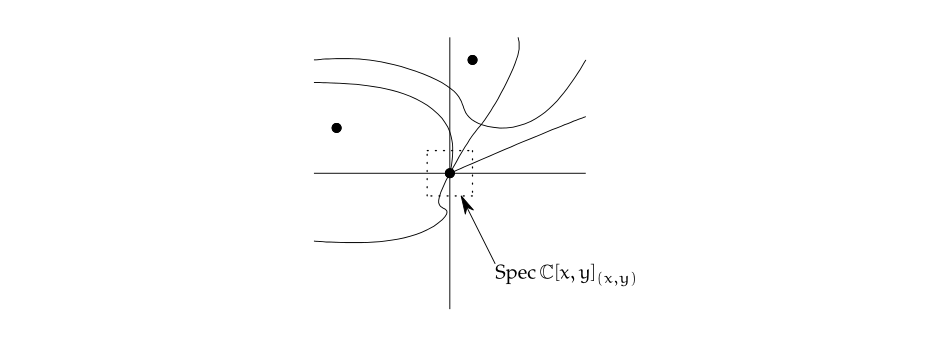
\includegraphics[width=\linewidth,height=\textheight,keepaspectratio]{Figures/localisation.png}
                                \caption{Localisation produces Zariski-open subsets (\cite{risingsea}, figure 3.5)}
                                \label{fig: zariski_open_via_localisation}
                            \end{figure}
                    \end{example}
                    
                    \begin{remark}[A reminder about limits of sheaves and of presheaves] \label{remark: sheaf_limits}
                        A Grothendieck topos $\E$ (i.e. a sheaf topos) is, \href{https://ncatlab.org/nlab/show/Grothendieck+topos#definition}{\underline{by definition}}, one equipped with a \href{https://ncatlab.org/nlab/show/geometric+embedding}{\underline{geometric embedding}} into a presheaf topos:
                            $$
                                \begin{tikzcd}
                                	\E & {\Psh_{\Sets}(\C)}
                                	\arrow[""{name=0, anchor=center, inner sep=0}, shift right=2, hook, from=1-1, to=1-2]
                                	\arrow[""{name=1, anchor=center, inner sep=0}, "{}^{\sh}(-)"', shift right=2, from=1-2, to=1-1]
                                	\arrow["\dashv"{anchor=center, rotate=-90}, draw=none, from=1, to=0]
                                \end{tikzcd}
                            $$
                        and due to this definition, or more precisely, because of the fact that the left-adjoint component of a geometric morphism (the sheafification functor ${}^{\sh}(-)$ in this situation) is left-exact by definition, and that \href{https://ncatlab.org/nlab/show/adjoints+preserve+\%28co-\%29limits}{\underline{right-adjoints \textit{a priori} preserve limits}}, one can show that limits of sheaves and of their \say{underlying presheaves} coincide. Particularly, in the event that \say{the} underlying site of $\E$ - say $(\C, J)$ - is \textit{subcanonical} and \textit{complete}, this would force the full subcategory of $\E$ consisting representable sheaves on $(\C, J)$ to be complete as well, thanks to the fact that \href{https://ncatlab.org/nlab/show/hom-functor+preserves+limits}{\underline{the Yoneda embedding preserves limits}}. 
                    \end{remark}
                    \begin{lemma}[On the completeness of affine scheme categories] \label{lemma: affine_scheme_limits} \index{Limits! of affine schemes}
                        Fix a base commutative ring $k$. Then, the category $\Sch^{\aff}_{/\Spec k}$ of affine schemes over $\Spec k$ is complete.
                    \end{lemma}
                        \begin{proof}
                            This comes directly from the discussion in remark \ref{remark: sheaf_limits}, since the Zariski site ${}^{k/}\Comm\Alg^{\op}_{\Zar}$ is subcanonical (cf. corollary \ref{theorem: zariski_coverages}) and since the category ${}^{k/}\Comm\Alg$ of commutative $k$-algebras is cocomplete (and hence the opposite category ${}^{k/}\Comm\Alg^{\op}$ is complete).
                        \end{proof}
                        
                \paragraph{\'Etale and smooth descent} \label{paragraph: etale_descent} \index{Topology!\'etale} \index{Topology!smooth}
                    \begin{remark}[Smooth sieves and \'etale sieves] \label{remark: smooth_and_etale_sieves}
                        For now extrapolate from proposition \ref{prop: compositions_and_base_changes_of_smooth_morphisms} and corollary \ref{coro: compositions_and_base_changes_of_etale_morphisms}.
                    \end{remark}
                
                \paragraph{Fppf descent} \index{Topology!fppf}
                
                \paragraph{Fpqc descent} \index{Topology!fpqc}
                    Before we discuss the so-called fpqc topology, let us first define the term \say{fpqc}, as well as investigate some basic properties of fpqc morphisms.
                    
                    \begin{definition}[Fpqc morphisms] \label{def: fpqc_morphisms} 
                        Fix a base commutative ring $k$. An affine-schematic morphism:
                            $$f: \calY \to \calX$$
                        of prestacks in $[\Spec k]$ is said to be \textbf{fpqc} (which stands for \textit{fid\`element plat et quasi-compacte} and translate into \say{faithfully flat and quasi-compact}) if and only if the corresponding $k$-algebra map is (surprise!) faithfully flat and quasi-compact in the Zariski topology.
                    \end{definition}
                    
                    \begin{remark}[Quasi-compact affine-schematic morphisms] \label{remark: quasi_compact_affine_schematic_morphisms} 
                        Let $k$ be a base commutative ring and let $R$ be a $k$-algebra defined by the ring homomorphism:
                            $$\varphi: k \to R$$
                        Now, recall that a scheme (or rather, its structural morphism) is \textbf{quasi-compact} if and only if any Zariski covering thereof can be refined by a finite one. Then, following theorem \ref{theorem: zariski_coverages}, a ring map such as $\varphi: k \to R$ is quasi-compact (or rather, the corresponding morphism of affine schemes is) if and only if any Zariski covering of $\Spec R$ can be decomposed into a finite cover of the following form:
                            $$\coprod_{i = 1}^n \Spec R_{x_i} \to \Spec R$$
                        and thus $R$ must be finitely generated by $n$ generators $x_1, ..., x_n$ as a $k$-algebra. By definition, this means that there exists a surjective ring homomorphism:
                            $$\pi: k[x_1, ..., x_n] \twoheadrightarrow R$$
                        which is equivalent to saying $R$ is isomorphic to $\frac{k[x_1, ..., x_n]}{\ker \pi}$, thanks to the First Isomorphism Theorem. 
                    \end{remark}
                    \begin{lemma}[Compositions and base changes of fpqc morphisms] \label{lemma: fpqc_compositions_and_base_changes}
                        Since fpqc morphisms are first and foremost affine-schematic, let us restrict our attention to fpqc morphisms between affine scheme (or actually, to fpqc ring maps).
                        \begin{enumerate}
                            \item \textbf{(Compositions):} Compositions of fpqc ring maps, such as:
                                $$
                                    \begin{tikzcd}
                                    	A & B & C
                                    	\arrow["\varphi", from=1-1, to=1-2]
                                    	\arrow["\psi", from=1-2, to=1-3]
                                    \end{tikzcd}
                                $$
                            are fpqc themselves too.
                            \item \textbf{(Base changes):} Let $\varphi: A \to B$ be an fpqc ring map and let $\psi: A \to A'$ be an arbitrary homomorphism between commutative rings. Then, the pushout $B \tensor_{\varphi, A, \psi} A'$ is fpqc over $A'$.  
                        \end{enumerate}
                    \end{lemma}
                        \begin{proof}
                            \noindent
                            \begin{enumerate}
                                \item \textbf{(Compositions):}  
                                    \begin{enumerate}
                                        \item \textbf{(Faithful flatness):} First of all, because a ring map:
                                            $$\varphi: A \to B$$
                                        is faithfully flat if and only if the functor $- \tensor_A B_0$ is faithful and left-exact, where $B_0 \cong \frac{B}{\ker \varphi}$, and because compositions of faithful (respectively left-exact) functors are also faithful (respectively left-exact), compositions of faithfully flat ring maps (or more generally, faithfully flat module homomorphisms for that matter) need to also be faithfully flat.
                                        \item \textbf{(Quasi-compactness):} Since $B$ is quasi-compact over $A$ and $C$ is quasi-compact over $B$, by assumption, we get via an application of remark \ref{remark: quasi_compact_affine_schematic_morphisms} that:
                                            $$B \cong \frac{A[x_1, ..., x_n]}{\ker \alpha}$$
                                        where $\alpha: A[x_1, ..., x_n] \to B$ is some surjective ring homomorphism, and subsequently, that:
                                            $$C \cong \frac{B[y_1, ..., y_m]}{\ker \beta} \cong \frac{\frac{A[x_1, ..., x_n, y_1, ..., y_m]}{\ker \alpha}}{\ker \beta} \cong \frac{A[x_1, ..., x_n, y_1, ..., y_m]}{\ker \alpha + \ker \beta}$$
                                        Then clearly, $C$ is finitely generated as an $A$-algebra, and therefore the composition:
                                            $$\psi \circ \varphi: A \to C$$
                                        is quasi-compact.
                                    \end{enumerate}
                                By putting everything together, we get that compositions of fpqc morphisms are necessarily fpqc themselves.
                                \item \textbf{(Base changes):} From above, we know there exists a natural integer $n$ along with a surjective $A$-algebra homomorphism:
                                    $$\alpha: A[x_1, ..., x_n] \to B$$
                                Then, let us make use of the fact that the functor $- \tensor_A A'$, by virtue of being a left-adjoint, preserves colimits to see that pushing out along $\psi: A \to A'$ preserves the surjectiveness of $\alpha$ into the following surjective $A'$-algebra homomorphism:
                                    $$\alpha': A'_0[x_1, ..., x_n] \to B \tensor_{\varphi, A, \psi} A'$$
                                wherein $A'_0 \cong \frac{A'}{\ker \psi}$. It thus remains to show that $\frac{A'_0[x_1, ..., x_n]}{\ker \alpha}$ is faithfully flat over $A'$. For that, consider firstly the following:
                                    $$
                                        \begin{aligned}
                                            \frac{A'_0[x_1, ..., x_n]}{\ker \alpha} & \cong \frac{\frac{A'[x_1, ..., x_n]}{\ker \psi}}{\ker \alpha}
                                            \\
                                            & \cong \frac{A'[x_1, ..., x_n]}{\ker \psi + \ker \alpha}
                                            \\
                                            & \cong \frac{A'[x_1, ..., x_n]}{\ker \psi} \tensor_A \frac{A'[x_1, ..., x_n]}{\ker \alpha}
                                            \\
                                            & \cong \frac{A'[x_1, ..., x_n]}{\ker \psi} \tensor_A \left(\frac{A[x_1, ..., x_n]}{\ker \alpha} \tensor_A \frac{A'}{\ker \psi}\right)
                                            \\
                                            & \cong \frac{A[x_1, ..., x_n]}{\ker \alpha} \tensor_A \frac{A'}{\ker \psi}
                                            \\
                                            & \cong B \tensor_A \frac{A'}{\ker \psi}
                                        \end{aligned}
                                    $$
                                
                            \end{enumerate}
                        \end{proof}
                
                    There are certain set-theoretic issues related to the fpqc topology, stemming from the fact that fpqc coverings are not locally finitely presented (smooth, \'etale, and fppf coverings are locally finitely presented for more or less trivial reasons; for an explanation of why Zariski coverings are locally finitely presented, see theorem \ref{theorem: zariski_coverages}). But to address and subsequently mitigate them, we will first need some notions from set theory, as well as a demonstration of how this topology is not very well-behaved.
                    
                    \begin{example}[An fpqc pathology]
                        
                    \end{example}
                    
                    \begin{definition}[Weak multi-limits and WISC] \label{def: weak_multilimits}
                        \noindent
                        \begin{enumerate}
                            \item \textbf{(Weak multi-limits):} Let:
                                $$F: \D \to \C$$
                            be a diagram in some arbitrary category $\C$. Then, its \textbf{weak multi-limit} is a small set $W$ of cones over $F$ (i.e. functors $\pt \to \C_{/F}$) such that any arbitrary cone $C$ factors through some element of $W$; neither the element of $W$ nor the factorisation itself is required to be unique. 
                            
                            Every diagram in a small category admits a weak multilimit.
                            \item \textbf{(Weakly Initial Set of Covers (WISC)):} Weak multi-colimits of empty diagrams (should they exist) are known as \textbf{weakly initial objects}.   
                        \end{enumerate}
                    \end{definition}
            
        \subsection{Reconciling the two approaches}
            \subsubsection{Structure sheaves}
                Next, we will be discussing the idea of so-call \textbf{structure sheaves}, but in order to make sense of these entities, we will need to know what $\C$-valued sheaves are for categories $\C$ more general than $\Sets$:
                \begin{definition}[$\C$-valued sheaves] \label{def: C_valued_sheaves}
                    This definition is an adaptation of definition 2.6 in \cite{nlab:sheaf} so that our sheaves might take values in categories other than $\Sets$.
                    \begin{enumerate}
                        \item \textbf{($\C$-valued sheaves):} Let $(\S, J)$ be a site (that is not necessarily small, as cases such as $\S \cong \Top$ and $\S \cong \Mfd^{\smooth}_{/\R}$ are interesting in their own rights) and let $\C$ be a category with \textit{enough small limits} and \textit{enough filtered colimits} (the purpose of the second hypothesis is to ensure that stalks, should they exist, are well-defined); note that $\C$ need not be small. Additionally, fix an \textit{arbitrary} object $x$ of $\S$ along with a covering sieve $\U_{/x} \in J$ thereon. Also, let:
                            $$j: \S \to \Psh_{\C}(\S)$$
                        be the Yoneda embedding. Then, a \textbf{$\C$-valued sheaf} on $(\S, J)$ is a functor:
                            $$\calF: \S^{\op} \to \C$$
                        such that:
                            $$\calF x \cong \calF \underset{u \in \U_{/x}}{\colim} ju$$
                        \item \textbf{($\C$-topoi):} $\C$-valued sheaves on a given site $(\S, J)$ form a category in the obvious manner. We shall be writing $\Sh_{\C}(\S, J)$ for this category, and such categories will be called \textbf{$\C$-topoi}, even though this is an abuse of terminology.
                    \end{enumerate}
                \end{definition}
                \begin{example}[Sheaves of rings]
                    The notion of sheaves of rings, which subsumes that of structure sheaves (cf. proposition \ref{prop: structure_sheaf}), follows suite from definition \ref{def: C_valued_sheaves}. Note that such constructions are well-defined, as the category of rings is both complete and cocomplete.
                \end{example}
                
                Having defined sheaves that might take values categories other than $\Sets$, let us now try to define affine schemes as locally ringed spaces whose underlying topological spaces are spectra of commutative rings, and whose structure presheaves have a certain condition imposed upon them, which happens to guarantee that:
                    \begin{enumerate}
                        \item these structure presheaves are indeed sheaves (proposition \ref{prop: structure_sheaf}) with local stalks (corollary \ref{coro: structure_sheaf_properties}), and
                        \item they are unique (proposition \ref{prop: structure_sheaf_uniqueness}), which is an important feature, because ringed spaces are uniquely defined by their structure sheaves; this fact will also be used to establish the fully faithfulness of $\Spec$ as a functor from $\Cring^{\op}$ to the category $\Spc^{\ringed, \loc}$ of locally ringed spaces. 
                    \end{enumerate}
                Our efforts will culminate in definition \ref{def: zariski_topoi}, along with remarks \ref{remark: affine_schemes_are_locally_ringed_spaces} and \ref{remark: affine_scheme_morphisms}. 
                    
                \begin{proposition}[Structure sheaves of affine schemes] \label{prop: structure_sheaf} \index{Structure sheaves}
                    Let $k$ be a base commutative ring, and let $\calO_{\Spec R}$ be \textit{a} presheaf of commutative rings on $\T^{\open}_{\Zar}(\Spec R)$ determined by the following rule on objects:
                        $$\calO_{\Spec R}(D_R(f)) \cong R_f$$
                    for all element $f \in R$. Any presheaf on $\T^{\open}_{\Zar}(\Spec R)$ that are defined this way is a Zariski sheaf (i.e. a sheaf on the site $\T^{\open}_{\Zar}(\Spec R)$ of Zariski-open subsets of $\Spec R$), and is called \textit{a} \textbf{structure sheaf} on $\Spec R$.
                \end{proposition}
                    \begin{proof}
                        Let $\U_{/\Spec R}$ be a sieve on $\T^{\open}_{\Zar}(\Spec R)$ that covers $U$, which is necessarily a set $\{D_R(f_{\alpha}) \hookrightarrow \Spec R\}_{\alpha \in A}$ of open subsets of $\Spec R$ indexed some set $\{f_{\alpha}\}_{\alpha \in A}$ of generators of $R$ (see lemma \ref{lemma: limits_indexed_by_generators} for an explanation of why this is the case). Then, consider the following:
                            $$
                                \begin{aligned}
                                    \calO_{\Spec R}(\Spec R) & \cong \calO_{\Spec R}(D_R(1))
                                    \\
                                    & \cong R_1
                                    \\
                                    & \cong R
                                    \\
                                    & \cong \underset{\alpha \in A}{\lim} R_{f_{\alpha}} \: \text{(cf. lemma \ref{lemma: limits_indexed_by_generators})}
                                    \\
                                    & \cong \underset{\alpha \in A}{\lim} \calO_{\Spec R}(D_R(f_{\alpha}))
                                \end{aligned}
                            $$
                    \end{proof}
                \begin{corollary}
                    By applying proposition \ref{prop: structure_sheaf}, corollary \ref{coro: zariski_frames_and_sites}, and remark \ref{remark: big_and_small_zariski_sites}, one can see that structure sheaves on ring spectra are also $\Cring$-valued sheaves on $\Cring^{\petit, \op}_{\Zar}$. This fact will come in handy when we try to establish Zariski topoi as locally ringed topoi in definition \ref{def: zariski_topoi}.
                \end{corollary}
                \begin{corollary}[On the locality of stalks] \label{coro: structure_sheaf_properties}
                    Let $R$ be a commutative ring and let $\p$ be an arbitrary prime ideal of $R$. Then one has the following characterisation of the stalk $\calO_{\Spec R, \p}$ at $\p$ of the structure sheaf $\calO_{\Spec R}$:
                        $$\calO_{\Spec R, \p} \cong R_{\p}$$
                    This shows that affine schemes are, in fact, \textit{locally} ringed spaces and not just ringed spaces. 
                \end{corollary} 
                    \begin{proof}
                        Recall that the stalk $\calF_x$ of a sheaf (of sets) $\calF$ on a topological space $(X, \T(X))$ is given by the filtered colimit indexed by the poset of open neighbourhoods of the chosen point $x \in X$:
                            $$\calF_x \cong \underset{U \in \{V \in \T(X) \mid V \ni x\}}{\colim} \calF(U)$$
                        By adapting this definition to the underlying Zariski-topological spaces of affine schemes, we get that:
                            $$\calO_{\Spec R, \p} \cong \underset{U \in \{V \in \T_{\Zar}^{\open}(\Spec R) \mid V \ni \p\}}{\colim} \calO_{\Spec R}(U)$$
                        with $\T_{\Zar}^{\open}(\Spec R)$ the Zariski topology defined via open sets as in definition \ref{def: zariski_open}. In corollary \ref{coro: zariski_basis}, we have already seen how the distinguished Zariski-open sets defined in definition \ref{def: zariski_open} form a basis for the Zariski topology on commutative ring spectra, and so the above filtered colimit can be rewritten as:
                            $$\calO_{\Spec R, \p} \cong \underset{D_R(f) \in \{V \in \T_{\Zar}^{\open}(\Spec R) \mid V \ni \p\}}{\colim} \calO_{\Spec R}\left(D_R(f)\right)$$
                        and because $D_R(f) = \{\p \in \Spec R \mid \p \not \ni f\}$, one subsequently gets:
                            $$\calO_{\Spec R, \p} \cong \underset{f \in \{g \in R \mid g \not \in \p\}}{\colim} \calO_{\Spec R}\left(D_R(f)\}\right)$$
                        Lastly we have the following isomorphism:
                            $$\calO_{\Spec R, \p} \cong \underset{f \in \{g \in R \mid g \not \in \p\}}{\colim} \calO_{\Spec R}\left(D_R(f)\right) \cong \underset{f \in R \setminus \p}{\colim} R_f \cong R_{\p}$$
                        Thus:
                            $$\calO_{\Spec R, \p} \cong R_{\p}$$
                        as claimed.
                    \end{proof}
                    
                \begin{proposition}[Uniqueness of structure sheaves] \label{prop: structure_sheaf_uniqueness}
                    Let $R$ be a commutative ring. Then, there is only one unique structure sheaf attached to $\Spec R$. 
                \end{proposition}
                    \begin{proof}
                        Suppose to the contrary that there exist two \textit{distinct} Zariski sheaves of $R$-algebras on ${}^{R/}\Comm\Alg^{\op}$ $\calF$ and $\calG$ such that:
                            $$\forall f \in R: \calF(\Spec R_f) \cong \calG(\Spec R_f) \cong R_f$$
                        However, the localisation of any commutative at its multiplicative identity is just itself, and so:
                            $$\calF(\Spec R) \cong \calG(\Spec R) \cong R$$
                        for all commutative rings $R$. This means that the functors $\calF$ and $\calG$ are naturally isomorphic, i.e. they can not be distinct. Thus, the structure sheaf attached to a given ring spectrum is unique (up to natural isomorphisms, of course).
                    \end{proof}
                    
                \begin{example}[Spotting structure sheaves in the wild]
                    Let $R$ be a discrete valuation ring that is a \href{https://en.wikipedia.org/wiki/Dedekind_domain}{\underline{Dedekind domain}} (so the only proper ideals of $R$ would be $(0)$ and its unique maximal ideal) with unique maximal ideal $\p$, and recall that its spectrum is (homeomorphic to) the Sierpi\'nski space (see example \ref{example: nonisomorphic_rings_with_the_same_spectra} for more details); in particular, the subset $\{(0)\}$ of $\Spec R = \{(0), \p\}$ is the only non-empty open proper subset. Now, suppose that $\calF$ is a Zariski sheaf on $\Spec R$ given by the following formula:
                        $$
                            \calF(U) \cong 
                            \begin{cases}
                                \text{$R$ if $U = \Spec R$}
                                \\
                                \text{$\Frac R$ if $U = \{(0)\}$}
                            \end{cases}
                        $$
                    (note that discrete valuation rings are integral domains, so it makes sense to consider their fields of fractions). The point that is to be made here is that $\calF$ qualifies as a structure sheaf on $\Spec R$. To see why this is the case, note that because $R$ has only two prime ideals, namely $(0)$ and $\p$, 
                \end{example}
                
                \begin{example}[The complex affine line]
                    Recall that in example \ref{example: spectra_sets}, we have seen how a point of the complex affine line $\A^1_{\bbC}$ is either the zero ideal, or of the form $(t - a)$ for any complex number $a$; one should keep the following picture in mind:
                        \begin{figure}[H]
    				        \centering
    				        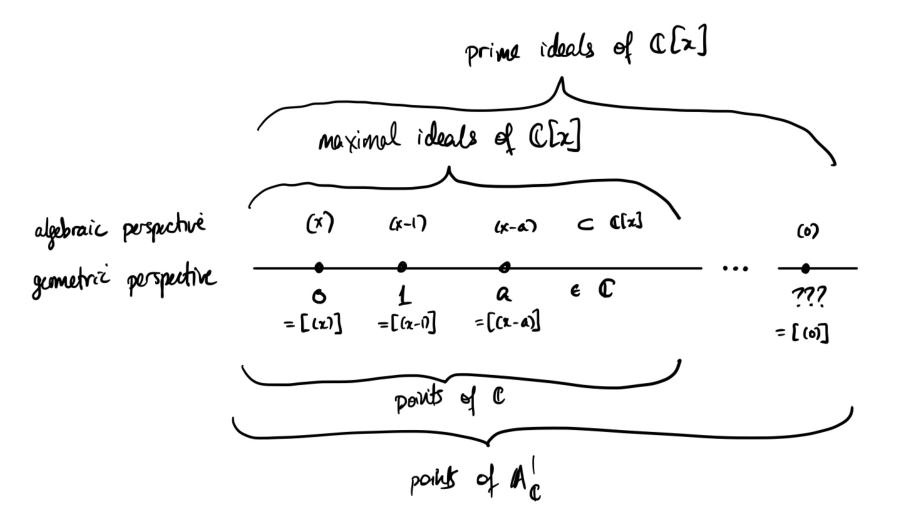
\includegraphics[width=\linewidth,height=\textheight,keepaspectratio]{Figures/complex affine line.png}
    				        \caption{The complex affine line $\A^1_{\bbC}$ (\cite{risingsea}, figure 3.1)}
    				        \label{fig: complex_affine_line_stalks}
    				    \end{figure}
				    \noindent
				    Now, as an affine scheme, $\A^1_{\bbC}$ comes equipped with a structure sheaf $\calO_{\A^1_{\bbC}}$, whose stalks, as shown in corollary \ref{coro: structure_sheaf_properties}, are precisely the localisations of $\bbC[t]$ at its prime ideals. There are thus two cases:
				        \begin{enumerate}
				            \item The stalk at $(0)$ is given by:
				                $$\calO_{\A^1_{\bbC}, (0)} \cong \bbC[t]_{(0)} \cong \bbC(t)$$
			                and thus the residue field is trivially $\bbC(t)$.
				            \item At non-zero primes, the stalks of the structure sheaf $\calO_{\A^1_{\bbC}}$ are given by the following localisations:
				                $$\calO_{\A^1_{\bbC}, (t - a)} \cong \bbC[t]_{(t - a)}$$
			                whose elements we note to be fractions of the form $\frac{f(t)}{g(t)}$ whose denominators do not vanish at $t = a$. Now, recall that the localisation of any commutative ring at a prime ideal is a local ring, and that inside \textit{any} local commutative ring, elements in the complement of the unique maximal ideal are units; in particular, these facts imply that the elements of the complement $\bbC[t]_{(t - a)} \setminus (t - a)\bbC[t]_{(t - a)}$ are all invertible. Consequently, these elements must be fractions $\frac{f(t)}{g(t)}$ whose numerators and denominators both do not vanish at $t = a$. Thus, a reasonable description of the canonical quotient map is the evaluation map:
			                    $$\frac{f(t)}{g(t)} \mapsto \frac{f(a)}{g(a)}$$
		                    whose image is precisely $\bbC$. Therefore, the stalks of $\calO_{\A^1_{\bbC}}$ are all equal to $\bbC$ (incidentally, this means that $\calO_{\A^1_{\bbC}}$, or the structure sheaf of the affine line over any algebraically closed field for that matter, is a \href{https://en.wikipedia.org/wiki/Local_system}{\underline{local system}}).
				        \end{enumerate}
                \end{example}
                
                \begin{definition}[\textcolor{red}{\textbf{\underline{\textbf{IMPORTANT}}}} Zariski topoi] \label{def: zariski_topoi} \index{Topoi!Zariski}
                    \noindent
                    \begin{enumerate}
                        \item \textbf{(Zariski topoi):} Let $k$ be a base commutative ring. Then, let us define the \textbf{small Zariski topos} over $\Spec k$ (or rather, over the Zariski site $\Comm\Alg^{\petit, \op}_{k, \Zar}$) as the sheaf topos above this site, which will often written $(\Spec k)_{\Zar}$, or in cases where sizes are of concern, $(\Spec k)_{\Zar}^{\petit}$; we shall also only be saying \say{Zariski topoi} instead of \say{small Zariski topoi} as in practice, it is mostly the former that will come up. Note that this topos can \textit{a priori} be turned into a \href{https://ncatlab.org/nlab/show/locally+ringed+topos}{\underline{locally ringed topos}} with structure sheaf being \textit{the} structure sheaf $\calO_{\Spec k}$ on $\Spec k$.
                        \item \textbf{(Affine schemes):} The category $\Sch^{\aff}_{/\Spec k}$ of affine schemes over $\Spec k$ is the image of ${}^{k/}\Comm\Alg^{\op}$ under the Yoneda embedding. 
                    \end{enumerate}
                \end{definition}
                
                \begin{remark}[On relativisation]
                    In the same way that ${}^{k/}\Comm\Alg^{\petit, \op}$ is equivalent to the slice category $\Cring^{\petit, \op}_{/\Spec k}$ for all commutative rings $k$, given any base ring spectrum $\Spec k$ and any $k$-algebra $R$, the Zariski topos $(\Spec R)_{\Zar}$ is nothing but the slice $\Sh_{\Sets}({}^{R/}\Comm\Alg_{\Zar}^{\petit, \op})_{/\Spec R}$. Naturally, one has \say{absolute} Zariski topoi, namely those equivalent to $(\Spec \Z)_{\Zar}$.
                \end{remark}
                
                \begin{remark}[Affine schemes are Zariski sheaves] \label{remark: affine_schemes_are_zariski_sheaves}
                    There is an equivalence of categories whose role in algebraic geometry can hardly be overstated, that being the equivalence between the category of commutative rings and that of affine schemes (over $\Spec \Z$). Now, given definition \ref{def: zariski_topoi}, this equivalence of categories is rather evident, as $\Sch^{\aff}$ is little more than the image of $\Cring^{\op}$ under the \textit{fully faithful} Yoneda embedding of the latter category. However, what is not entirely self-explanatory is the fact that \textit{affine schemes are sheaves} on $\Cring^{\petit, \op}_{\Zar}$, although showing this to be true is actually not very difficult: simply recall that every commutative ring $R$ can be written as the (small and filtered) colimit of all finitely presented commutative $R$-algebras:
                    \cite[\href{https://stacks.math.columbia.edu/tag/0BUF}{Tag 0BUF}]{stacks}, which implies that:
                        $$
                            \begin{aligned}
                                \Cring^{\op}(-, R) & \cong \Cring^{\op}\left(-, \underset{P \in {}^{R/}\Comm\Alg^{\petit, \op}}{\lim} P\right)
                                \\
                                & \cong \underset{P \in {}^{R/}\Comm\Alg^{\petit, \op}}{\lim} \Cring^{\op}(-, P)
                                \\
                                & \cong \underset{P \in {}^{R/}\Comm\Alg^{\petit, \op}}{\lim} \Cring^{\petit, \op}(-, P)
                            \end{aligned}
                        $$
                    (the last isomorphism holds because $\Cring^{\petit}$ is a \textit{full} subcategory of $\Cring$; cf. remark \ref{remark: big_and_small_zariski_sites}), and then, by applying this limit of representables to the colimit of a covering sieve $\U_{/S}$ on an object $S$ of $\Cring^{\petit, \op}_{\Zar}$, we will get:
                        $$
                            \begin{aligned}
                                \Cring^{\op}(\colim \U_{/S}, R) & \cong \Cring^{\op}\left(-, \underset{P \in {}^{R/}\Comm\Alg^{\petit, \op}}{\lim} P\right)
                                \\
                                & \cong \underset{P \in {}^{R/}\Comm\Alg^{\petit, \op}}{\lim} \Cring^{\petit, \op}(\colim \U_{/S}, P)
                                \\
                                & = \underset{P \in {}^{R/}\Comm\Alg^{\petit, \op}}{\lim} \underset{U \in \U_{/S}}{\lim} \Cring^{\petit, \op}(U, P)
                            \end{aligned}
                        $$
                    which tells us that the affine scheme $\Cring^{\op}(-, R)$ is a sheaf on $\Cring^{\petit, \op}_{\Zar}$, since the Zariski coverage is subcanonical (cf. theorem \ref{theorem: zariski_coverages}) - which implies that the functors $\Cring^{\petit, \op}(-, P)$ are sheaves on $\Cring^{\petit, \op}_{\Zar}$ - and because limits of sheaves are still sheaves. 
                    
                    It should also be noted that representable functors on $\Cring^{\petit, \op}$ are sheaves on $\Cring^{\petit, \op}_{\Zar}$, as the Zariski coverage is subcanonical (see theorem \ref{theorem: zariski_coverages}), and that these sheaves are \textit{a priori} affine schemes (because finitely presented commutative rings are still commutative rings), but \textit{not all affine schemes are representable} as sheaves on the small Zariski site, since $\Cring^{\petit}$ is a full subcategory of $\Cring$ (see remark \ref{remark: big_and_small_zariski_sites}).
                \end{remark}
                
                Next, we will discuss how our definition of affine schemes (definition \ref{def: zariski_topoi}) is congruent with the traditional one, which states that affine schemes are locally ringed spaces whose underlying topological spaces are prime spectra of commutative rings. For starters, let us review the notion of ringed spaces and locally ringed spaces:
                \begin{definition}[Ringed spaces] \label{def: ringed_spaces}
                    \noindent
                    \begin{enumerate}
                        \item \textbf{(Ringed spaces):} Let $X$ be a topological space with topology $\T(X)$ and let $\calO_X$ be a \textit{fixed} sheaf of rings on the site $\T(X)^{\op}$ of open subsets of $X$. Then, the pair $(X, \calO_X)$ is known as a \textbf{ringed space}, with $\calO_X$ known as the \textbf{structure sheaf}.
                        \item \textbf{(Locally ringed spaces):} If in addition, the stalks $\calO_{X, x}$ at points $x \in X$, given by the following filtered colimit over open neighbourhoods $U$ of $x$:
                            $$\calO_{X, x} := \underset{U \in \{V \in \T(X) \mid V \ni x\}}{\colim} \calO_X(U)$$
                        are local rings, then $(X, \calO_X)$ will be known as a \textbf{locally ringed space}.
                    \end{enumerate}
                \end{definition}
                \begin{remark}[The category of (locally) ringed spaces] \label{remark: cateogry_of_ringed_spaces}
                    Ringed spaces and locally ringed spaces form categories, denoted by $\Spc^{\ringed}$ and $\Spc^{\ringed, \loc}$ respectively; note that the latter is not a full subcategory of the former. See remark \ref{remark: affine_schemes_are_locally_ringed_spaces} for more details, particularly on how morphisms in these categories are defined.
                \end{remark}
                \begin{example}
                    A very important feature of (locally) ringed spaces is that they are uniquely determined, up to natural isomorphisms, by their structure sheaves. For instance, a topological manifold equipped with a sheaf of smooth functions is a different ringed space from that very same manifold equipped with a sheaf of analytic functions. Also, the structure sheaf tends not to define the underlying topological space; this happens for (affine) schemes, which is why categories thereof are interesting.
                \end{example}
                
                \begin{remark}[Affine schemes are locally ringed spaces] \label{remark: affine_schemes_are_locally_ringed_spaces}
                    \noindent
                    \begin{enumerate}
                        \item \textbf{(Putting together the locally ringed spaces):} Recall that in corollary \ref{theorem: zariski_coverages}, we have seen how the Zariski sieves covering the spectrum of a commutative ring generate a coverage on $\Cring^{\op}$, and furthermore, that the resultant Zariski site $\Cring^{\op}_{\Zar}$ is subcanonical. Thus, one might as well think of affine schemes as prime spectra of commutative rings, thanks to Yoneda's lemma. This means that an affine scheme can be assumed to naturally possess an underlying topological space (and hence set) whose topology is the Zariski topology as described in definition \ref{def: zariski_closed} (or equivalently, definition \ref{def: zariski_open}; see proposition \ref{prop: zariski_topology_equivalence} for a proof of this equivalence). In conjunction with the fact that each ring spectrum comes equipped with a unique structure sheaf whose stalks are local rings, as established in proposition \ref{prop: structure_sheaf_uniqueness}, this implies that one can \textit{define} affine schemes to be locally ringed spaces of the form $(|\Spec R|, \calO_{\Spec R})$ (we are writing $|\Spec R|$ here instead of $\Spec R$ to put emphasis on the underlying topological space). In fact, this is the traditional definition that one can find in textbooks on schemes such as \cite{ega1} and \cite{hartshorne}. 
                        \item \textbf{(An incomplete construction of morphisms):} Let $f: \Spec B \to \Spec A$ be a morphism of affine schemes and consider an associated geometric morphisms between the ringed Zariski topoi $(\Spec A)_{\Zar}$ and $(\Spec B)_{\Zar}$:
                            $$
                                \begin{tikzcd}
                                	{f_*: (\Spec B)_{\Zar}} & {(\Spec A)_{\Zar}: f^*}
                                	\arrow[""{name=0, anchor=center, inner sep=0}, "f_*"', shift right=2, from=1-1, to=1-2]
                                	\arrow[""{name=1, anchor=center, inner sep=0}, "f^*"', shift right=2, from=1-2, to=1-1]
                                	\arrow["\dashv"{anchor=center, rotate=-90}, draw=none, from=1, to=0]
                                \end{tikzcd}
                            $$
                        Then, the structure sheaves $\calO_{\Spec A}$ and $\calO_{\Spec B}$ are related through natural morphisms that come from the adjunction $f^* \ladjoint f_*$:
                            $$f^{\sharp}: \calO_{\Spec A} \to f_*\calO_{\Spec B}$$
                            $$f^{\flat}: f^*\calO_{\Spec A} \to \calO_{\Spec B}$$
                        One can choose one of these canonical morphisms (for example, in \cite{hartshorne}, section II.2, it is asserted that the arrow $f^{\sharp}: \calO_{\Spec A} \to f_*\calO_{\Spec B}$ in $(\Spec A)_{\Zar}$ is the comorphism of sheaves associated to the ), and thus gets a morphism:
                            $$(|f|, f^{\sharp}): (|\Spec A|, \calO_{\Spec A}) \to (|\Spec B|, \calO_{\Spec B})$$
                        of ringed spaces, which can considered as being in bijective correspondence (or even the same as) \textit{the} morphism of affine schemes $f: \Spec B \to \Spec A$, provided that the choice of geometric morphism $(f^* \ladjoint f_*)$ between the ringed topoi $(\Spec B)_{\Zar}$ and $(\Spec A)_{\Zar}$ is fixed. 
                    \end{enumerate}
                \end{remark}
                    
                \begin{remark}[On structure sheaves and morphisms between affine schemes] \label{remark: affine_scheme_morphisms}
                    Actually, affine schemes are \textit{locally} ringed spaces, so the morphisms of ringed Zariski topoi and spaces induced by a morphism of affine schemes $f: \Spec B \to \Spec A$ had better be those between \textit{locally} ringed topoi and spaces. This is the case, but we will need to verify it via checking whether or not we can choose the geometric morphisms $(f^* \ladjoint f_*)$ between the ringed topoi $(\Spec B)_{\Zar}$ and $(\Spec A)_{\Zar}$ so that the associated comorphisms of sheaves $f^{\sharp}$ (or $f^{\flat}$ for that matter) are local homomorphisms at the level of stalks. To that end, let us first of all quickly review stalks, or even before doing so, the notion of points of topoi.
                        \begin{enumerate}
                            \item \textbf{(Points of topoi and stalks):} Recall firstly that $\Sets$, being equivalent to sheaf topoi on the singleton site, is a terminal object in the category $\Sh\Topos$ of Grothendieck topoi (see \cite{sga4}, subsection IV.2.2 or \cite{HTT}, proposition 6.3.4.1 for details). Let us then define a point $x$ of a Grothendieck topos $\E$ as a geometric morphism $(x^* \ladjoint x_*)$ from $\Sets$ to $\E$:
                                $$
                                    \begin{tikzcd}
                                    	{x_*: \Sets} & {\E: x^*}
                                    	\arrow[""{name=0, anchor=center, inner sep=0}, "x_*"', shift right=2, from=1-1, to=1-2]
                                    	\arrow[""{name=1, anchor=center, inner sep=0}, "x^*"', shift right=2, from=1-2, to=1-1]
                                    	\arrow["\dashv"{anchor=center, rotate=-90}, draw=none, from=1, to=0]
                                    \end{tikzcd}
                                $$
                            and subsequently, the \textbf{stalk} at $x$ of an object $F$ in $E$ as the inverse image $x^*F$. In the context of affine schemes, one might alternatively define the stalk a structure sheaf $\calO_{\Spec R}$ at a point $\p$ as a geometric morphism from the Zariski topos associated to the residue field $\kappa_{\p}$ to $(\Spec R)_{\Zar}$ (recall that spectra of fields are singletons, and thus sheaf topoi over them are all equivalent to $\Sets$):
                                $$
                                    \begin{tikzcd}
                                    	{\p_*: (\Spec \kappa_{\p})_{\Zar}} & {(\Spec R)_{\Zar}: \p^*}
                                    	\arrow[""{name=0, anchor=center, inner sep=0}, "\p_*"', shift right=2, from=1-1, to=1-2]
                                    	\arrow[""{name=1, anchor=center, inner sep=0}, "\p^*"', shift right=2, from=1-2, to=1-1]
                                    	\arrow["\dashv"{anchor=center, rotate=-90}, draw=none, from=1, to=0]
                                    \end{tikzcd}
                                $$
                            (this also plays nicely with how we tend to think of points as being the same as morphisms from spectra of residue fields thereon into the ambient affine schemes); note that the consideration of the Zariski is important here, as there are topologies on affine schemes, such as the \'etale topology, in which the site attached to the spectrum of a field need not be singleton: for instance, objects of the \'etale site associated to a field spectrum $\Spec K$ are the finite separable extensions of $K$; more on this later.
                            \item \textbf{(Stalks of comorphisms):} Now, this is all well and good, but what does it mean for the notion of morphisms between affine schemes given above ? Consider a morphism of affine schemes $f: \Spec B \to \Spec A$, viewed as that of representable sheaves on $\Cring^{\op}$. Naturally, they induce a morphism of ringed Zariski topoi $(f^* \ladjoint f_*): (\Spec B)_{\Zar} \to (\Spec A)_{\Zar}$, which in turn induce comorphisms of sheaves $f^{\sharp}: \calO_{\Spec A} \to f_*\calO_{\Spec B}$ and $f^{\flat}: f^*\calO_{\Spec A} \to \calO_{\Spec B}$; let us focus our attention on $f^{\sharp}$. Now, fix a point $\q \in |\Spec B|$. As discussed above, such a point gives a point $(\q^* \ladjoint \q_*)$ of the topos $(\Spec A)_{\Zar}$:
                                $$
                                    \begin{tikzcd}
                                    	{\q_*: (\Spec \kappa_{\q})_{\Zar}} & {(\Spec A)_{\Zar}: \q^*}
                                    	\arrow[""{name=0, anchor=center, inner sep=0}, "\q_*"', shift right=2, from=1-1, to=1-2]
                                    	\arrow[""{name=1, anchor=center, inner sep=0}, "\q^*"', shift right=2, from=1-2, to=1-1]
                                    	\arrow["\dashv"{anchor=center, rotate=-90}, draw=none, from=1, to=0]
                                    \end{tikzcd}
                                $$
                            and thus, one can take the stalk at $\q$ of the arrow $f^{\sharp}$ in $(\Spec A)_{\Zar}$:
                                $$f^{\sharp}_{\q} = \q^* f^{\sharp}: \q^*\calO_{\Spec A} \to \q^*f_*\calO_{\Spec B}$$ 
                            Now, because right-adjoints ($f_*$ in this case) are \textit{a priori} left-exact, and because the left-adjoint component of geometric morphisms ($\q^*$ in this case) are required to be left-exact, (commutative) ring objects naturally exist in topoi, as they are defined through products. Thus, $f^{\sharp}_{\q}: \q^*\calO_{\Spec A} \to \q^*f_*\calO_{\Spec B}$ can very well be a homomorphism between commutative rings (taking $f^{\flat}$ also works, because once again, the left-adjoint components of geometric morphisms left-exact by definition). And because affine schemes are locally ringed spaces, our tasks is now two-fold: to prove that stalks of the structure sheaves of Zariski topoi can indeed be local rings, and that stalks of comorphisms can be \href{https://proofwiki.org/wiki/Definition:Local_Ring_Homomorphism}{\underline{local homomorphism}} between local commutative rings. 
                            
                            One thing that will help us with the latter is the observation that $\q^*f_*\calO_{\Spec B}$ is the same as the stalk of $\calO_{\Spec A}$ at $f(\q)$ (this is also why we prefer $f^{\sharp}$ to $f^{\flat}$, as working with the latter along with a would result in having to \textit{choose} a point in $f^{-1}(\p)$, with $\p \in |\Spec A|$, where we can consider stalks). This should be evident, as the point $\left(f(\q)^* \ladjoint f(\q)_*\right)$ of the topos $(\Spec A)_{\Zar}$ fits nicely into the following commutative diagram in $\Sh\Topos$:
                                $$
                                    \begin{tikzcd}
                                    	\Sets & {(\Spec B)_{\Zar}} \\
                                    	& {(\Spec A)_{\Zar}}
                                    	\arrow["\q", from=1-1, to=1-2]
                                    	\arrow["f", from=1-2, to=2-2]
                                    	\arrow["{f(\q) = f \circ \q}"', dashed, from=1-1, to=2-2]
                                    \end{tikzcd}
                                $$
                            In conclusion, the stalk at a point $\q \in |\Spec B|$ of the comorphism $f^{\sharp}$ is the following morphism of commutative rings internal to the topos $(\Spec A)_{\Zar}$:
                                $$f^{\sharp}_{\q}: \q^*\calO_{\Spec A} \to f(\q)^*\calO_{\Spec B}$$
                            or in more traditional notations:
                                $$f^{\sharp}_{\q}: \calO_{\Spec A, \q} \to \calO_{\Spec B, f(\q)}$$
                            \item \textbf{(Interlude: A constructive take on local rings):} Consider a generic topos (not even necessarily a sheaf topos) $\E$ and let us suppose that a commutative ring object $R$ is \textbf{local} if and only if it is not trivial (i.e. non-zero) and whenever $x + y = 1_R$, either $x$ or $y$ is invertible; formally, these axioms read:
                                $$\E \vDash \left( (0_R = 1_R) \vdash \bot \right)$$
                                $$\E \vDash \left( (x + y = 1_R) \vdash \exists z: R.  (zx = 1_R) \vee (zy = 1_R) \right)$$
                            Next, to each such local ring, let us associate an object $\m_R$ of $\E$ given by:
                                $$\E \vDash \left(x: \m_R \dashv\vdash \forall y: R. (1_R - xy: R^{\x})\right)$$
                            wherein the group of units $R^{\x}$ come from the following adjunction:
                                $$
                                    \begin{tikzcd}
                                    	{\Ring(\E)} & {\Grp(\E)}
                                    	\arrow[""{name=0, anchor=center, inner sep=0}, "{(-)^{\x}}"', shift right=2, from=1-1, to=1-2]
                                    	\arrow[""{name=1, anchor=center, inner sep=0}, "{[-]}"', shift right=2, from=1-2, to=1-1]
                                    	\arrow["\dashv"{anchor=center, rotate=-90}, draw=none, from=1, to=0]
                                    \end{tikzcd}
                                $$
                            in which the right-adjoint component $[-]$ is the assignment of group algebras to groups; it is not hard to see that $\m_R$ would be a subobject of $R$. Then, given a pair of local rings $(R, \m_R), (S, \m_S)$ internal to $\E$, let us declare a local ring homomorphism from $(R, \m_R)$ to $(S, \m_S)$ to be a ring homomorphism $f: R \to S$ whose pullback along the canonical inclusion of $\m_S$ into $S$ is just $\m_R$. Thanks to the \href{https://ncatlab.org/nlab/show/pasting+law+for+pullbacks}{\underline{pasting law for pullbacks}}, it is not hard to see how local commutative rings and local homomorphisms form a category internal to $\E$, which we shall appropriately denote by $\Cring^{\loc}(\E)$. 
                            
                            Also, for the sake of making things more familiar, one can show that the object $\m_R$ associated to a local ring $R$ is first of all unique, and second of all, is the sole maximal ideal in the \href{https://stacks.math.columbia.edu/tag/07BH}{\underline{common definition of local rings}}.
                            \item \textbf{(Putting everything together):} We have already shown that given any morphism of affine schemes:
                                $$f: \Spec B \to \Spec A$$
                            along with a fixed point $\q \in |\Spec B|$, along with a choice of comorphism of sheaves $f^{\flat}: \calO_{\Spec A} \to f_*\calO_{\Spec B}$, the corresponding stalk $f^{\sharp}_{\q}: \calO_{\Spec A, \q} \to \calO_{\Spec B, f(\q)}$ at $\q$ is a commutative ring homomorphism. Now, because local rings form natural categories internal to topoi, and because affine schemes are locally ringed spaces (see remark \ref{remark: affine_schemes_are_locally_ringed_spaces}), it makes sense to require stalks of comorphisms of sheaves to be local homomorphisms. This, incidentally, tells us that affine schemes form a \textit{full} subcategory of the category $\Spc^{\ringed, \loc}$ of locally ringed spaces (which we note to be equivalent to the slice $\Spc^{\ringed, \loc}_{/(|\Spec \Z|, \calO_{\Spec \Z})}$), as morphisms of locally ringed spaces are precisely those between ringed spaces whose stalks of comorphisms are local ring homomorphisms (cf. \cite{hartshorne}, section II.2). 
                        \end{enumerate}
                \end{remark}
                
            \subsubsection{Global sections and the Fundamental Theorem of Algebraic Geometry} 
                Now, let us start working our way towards the Fundamental Theorem of Algebraic Geometry (theorem \ref{theorem: fundamental_adjunction}), and to begin, let us lay down one unifying notion of global sections of sheaves:
                \begin{definition}[Global sections] \index{Global sections}
                    Let $\C$ be a category with enough small limits and terminal objects $1$ (note that complete categories \textit{a priori} have terminal objects) and let $\E_{\C}$ be a $\C$-topos. Then, the global section functor on $\E_{\C}$, denoted by $\Gamma_{\E_{\C}}$ (or simply $\Gamma$ when $\C$ is fixed), is defined to be the covariant hom-functor $\E_{\C}(\underline{1}, -)$ out of the local system $\underline{1}$ with values in the terminal object $1$ (note that the local system $\underline{1}$ is terminal in $\E_{\C}$). 
                \end{definition}
                
                \begin{remark}[A slight technical modification] 
                    Our main result, theorem \ref{theorem: fundamental_adjunction}, is meant to be about an adjoint pair between $\Spc^{\ringed, \loc}$ and $\Cring^{\op}$, not $\Cring$, and this is a problem, because so far, we have been working with structure sheaves on ringed spaces (and particularly, affine schemes), as though they took values in $\Cring$. What to do, then ? The answer is simple: just go to the opposite category. $\Cring$ is a category which is both complete and cocomplete, which in particular, means that $\Cring^{\op}$ has enough limits (colimits in $\Cring$) and enough filtered colimits (filtered limits in $\Cring$). Hence, there is nothing preventing structure sheaves from taking values in $\Cring^{\op}$, and this is precisely idea of structure sheaf that we shall be working with from this point on. Requiring structure sheaves to take values in $\Cring^{\op}$ instead of $\Cring$ should not affect any of the previously established results - including, but not limited to proposition \ref{prop: structure_sheaf}, corollary \ref{coro: structure_sheaf_properties}, and proposition \ref{prop: structure_sheaf_uniqueness} - as what they are concerned with occur at the level of elements, not objects and arrows between them. 
                \end{remark}
                
                \begin{remark}[Global sections of ringed spaces]
                    Because each ringed space is uniquely determined by its structure sheaf, it makes sense to consider \say{global sections} of ringed spaces as though we were doing so for just structure sheaves thereof. Notationally, it is common to write:
                        $$\Gamma(X, \calO_X) := \Gamma(\calO_X)$$
                    for each ringed space $(X, \calO_X)$; whenever this happens, do keep in mind that the domain of $\Gamma$ is not $\Spc^{\ringed, \loc} \x \Sh_{\Cring^{\op}}(\T(X))$ (with $\T(X)$ the topology on $X$), but simply $\Sh_{\Cring^{\op}}(\T(X))$.   
                \end{remark}
                    
                The following, while written out as a lemma, is actually a particularly technical section of the proof that has been isolated for the sake of clarity:
                \begin{lemma}\label{lemma: adjunction_unit_ringed_spaces}
                    Let $(X, \calO_X)$ be a locally ringed space. Then, there is a canonical arrow:
                        $$\eta_X: (X, \calO_X) \to \left(|\Spec \Gamma(\calO_X)|, \calO_{\Spec \Gamma(\calO_X)}\right)$$
                    in $\Spc^{\ringed, \loc}$, which should be thought of as the evaluation of global functions on $X$ (i.e. elements of $\Gamma(\calO_X)$) at points therein.
                \end{lemma}
                    \begin{proof}
                        \noindent
                        \begin{enumerate}
                            \item \textbf{(Continuous map between underlying topological spaces):} Let $\T(X)$ denote the given topology on $X$ and let $\T^{\discrete}(X)$ denote the discrete topology. First of all, note that any function:
                                $$(X, \T^{\discrete}(X)) \to |\Spec \Gamma(\calO_X)|$$
                            must be continuous, as the preimage of any Zariski-open subset of $|\Spec \Gamma(\calO_X)|$, by virtue of being a subset of $X$, must be open according to the definition of the discrete topology. Thus, it shall suffice to show that there exists a continuous function:
                                $$(X, \T(X)) \to (X, \T^{\discrete}(X))$$
                            as a continuous function:
                                $$\eta_X: (X, \T(X)) \to |\Spec \Gamma(\calO_X)|$$
                            would then exist as the dashed arrow in the following commutative diagram in $\Top$:
                                $$
                                    \begin{tikzcd}
                                    	{(X, \T(X))} && {|\Spec \Gamma(\calO_X)|} \\
                                    	& {(X, \T^{\discrete}(X))}
                                    	\arrow[from=1-1, to=2-2]
                                    	\arrow[from=2-2, to=1-3]
                                    	\arrow["\eta_X", dashed, from=1-1, to=1-3]
                                    \end{tikzcd}
                                $$
                            However, note that there is nothing preventing us from simply letting the function $(X, \T(X)) \to (X, \T^{\discrete}(X))$ be the one that is the identity on the underlying sets, which is trivially continuous: in fact, the desired continuous function $(X, \T(X)) \to (X, \T^{\discrete}(X))$ is nothing but the evaluation of the unit of the following forgetful-free adjunction at the object $(X, \T(X))$ of $\Top$:
                                $$
                                    \begin{tikzcd}
                                    	\Top & \Sets
                                    	\arrow[""{name=0, anchor=center, inner sep=0}, shift right=2, from=1-1, to=1-2]
                                    	\arrow[""{name=1, anchor=center, inner sep=0}, shift right=2, from=1-2, to=1-1]
                                    	\arrow["\dashv"{anchor=center, rotate=-90}, draw=none, from=1, to=0]
                                    \end{tikzcd}
                                $$
                            (recall that discrete spaces are free topological spaces, and that free constructions are left-adjoints). As stated above, this implies the existence of a continuous function:
                                $$\eta_X: (X, \calO_X) \to |\Spec \Gamma(\calO_X)|$$
                            \item \textbf{(Comorphism between structure sheaves):} We need to demonstrate that there is a homomorphism of sheaves of commutative rings (i.e. a natural transformation between sheaves of rings):
                                $$\eta_X^{\sharp}: \calO_{\Spec \Gamma(\calO_X)} \to (\eta_X)_*\calO_X$$
                            whose stalks at points of $X$ are local homomorphisms between local rings (i.e. the stalks of the structure sheaves). To that end, suppose that:
                                $$(\eta_X)_*\calO_X(U) \cong \calO_X(\eta_X^{-1}U)$$
                            for all Zariski-open subsets $U$ of $|\Spec \Gamma(\calO_X)|$ (note that the expression $\calO_X(\eta_X^{-1}U)$ makes sense because we have shown that $\eta_X$ is continuous, which implies that the preimage $\eta_X^{-1}(U)$ of the open subset $U$ is open in $X$, per the definition of continuity). The goal is then to prove that there exist commutative diagrams as follows for all inclusions of Zariski-open subsets $U \hookrightarrow V$ of $|\Spec \Gamma(\calO_X)|$:
                                $$
                                    \begin{tikzcd}
                                    	{\calO_{\Spec \Gamma(\calO_X)}(U)} & {\calO_X(\eta_X^{-1}U)} \\
                                    	{\calO_{\Spec \Gamma(\calO_X)}(V)} & {\calO_X(\eta_X^{-1}V)}
                                    	\arrow["{\eta_X^{\sharp}(U)}", from=1-1, to=1-2]
                                    	\arrow["{\eta_X^{\sharp}(V)}", from=2-1, to=2-2]
                                    	\arrow[from=2-1, to=1-1]
                                    	\arrow[from=2-2, to=1-2]
                                    \end{tikzcd}
                                $$
                            and because the Zariski topology on $|\Spec \Gamma(\calO_X)|$ has a basis made up by the basic open sets $D_{\Gamma(\calO_X)}(f)$ (for all $f \in \Gamma(\calO_X)$), and also because $\calO_{\Spec \Gamma(\calO_X)}$ is a sheaf in the Zariski topology (cf. proposition \ref{prop: structure_sheaf}), it shall suffice to restrict ourselves to cases wherein $U$ is merely a basic open subset, which would mean showing that there exists commutative diagrams of the following form:
                                $$
                                    \begin{tikzcd}
                                    	{\calO_{\Gamma(\calO_X)}(D_{\Gamma(\calO_X)}(f))} && {\calO_X(\eta_X^{-1}D_{\Gamma(\calO_X)}(f))} \\
                                    	{\calO_{\Spec \Gamma(\calO_X)}(V)} && {\calO_X(\eta_X^{-1}V)}
                                    	\arrow["{\eta_X^{\sharp}(D_{\Gamma(\calO_X)}(f))}", from=1-1, to=1-3]
                                    	\arrow["{\eta_X^{\sharp}(V)}", from=2-1, to=2-3]
                                    	\arrow[from=2-1, to=1-1]
                                    	\arrow[from=2-3, to=1-3]
                                    \end{tikzcd}
                                $$
                            
                            Let $x \in X$ be a point that is contained inside a given preimage $\eta_X^{-1} D_{\Gamma(\calO_X)(f)}$. Its image under $\eta_X$ would then be the point $\eta_X(x) \in D_{\Gamma(\calO_X)}(f)$. Next, consider the following \textit{not-yet-commutative} diagram, wherein non-commutativity is emphasises through the dashed arrows:
                                $$
                                    \begin{tikzcd}
                                    	& {\calO_{\Spec \Gamma(\calO_X), \eta_X(x)}} && {\calO_{X, x}} \\
                                    	{\calO_{\Spec \Gamma(\calO_X)}(D_{\Gamma(\calO_X)}(f))} && {\calO_X(\eta_X^{-1}D_{\Gamma(\calO_X)}(f))} \\
                                    	{\calO_{\Spec \Gamma(\calO_X)}(V)} && {\calO_X(\eta_X^{-1}V)}
                                    	\arrow["{\eta_X^{\sharp}(D_{\Gamma(\calO_X)}(f))}", dashed, from=2-1, to=2-3]
                                    	\arrow["{\eta_X^{\sharp}(V)}", dashed, from=3-1, to=3-3]
                                    	\arrow[from=3-1, to=2-1]
                                    	\arrow[from=3-3, to=2-3]
                                    	\arrow[from=2-1, to=1-2]
                                    	\arrow[from=2-3, to=1-4]
                                    	\arrow["{\eta_{X, x}^{\sharp}}", from=1-2, to=1-4]
                                    	\arrow[from=3-3, to=1-4]
                                    	\arrow[from=3-1, to=1-2]
                                    \end{tikzcd}
                                $$
                            wherein:
                                $$\eta_{X, x}^{\sharp}: \calO_{\Spec \Gamma(\calO_X), \eta_X(x)} \to \calO_{X, x}$$
                            is the stalk map at $x$, and note that the triangular side faces commute thanks to the definition of stalks as certain (filtered) colimits. Now, observe that when $V \cong |\Spec \Gamma(\calO_X)|$, the \say{slanted} square at the back becomes commutative, as $\calO_{\Spec \Gamma(\calO_X)}(V)$ would then be nothing more than the global section $\Gamma(\calO_X)$, which comes equipped with a natural map into $\calO_{X}(\eta_X^{-1}|\Spec \Gamma(\calO_X)|)$, as the preimage $\eta_X^{-1} |\Spec \Gamma(\calO_X)|$ is an open subset of $X$ (thanks to the continuity of $\eta_X$):
                                $$
                                    \begin{tikzcd}
                                    	{\calO_{\Spec \Gamma(\calO_X), \eta_X(x)}} & {\calO_{X, x}} \\
                                    	{\Gamma(\calO_X)} & {\calO_X(\eta_X^{-1} |\Spec \Gamma(\calO_X)|)}
                                    	\arrow["{\eta_X^{\sharp}(|\Spec \Gamma(\calO_X)|)}", from=2-1, to=2-2]
                                    	\arrow["{\eta_{X, x}^{\sharp}}", from=1-1, to=1-2]
                                    	\arrow[from=2-2, to=1-2]
                                    	\arrow[from=2-1, to=1-1]
                                    \end{tikzcd}
                                $$
                            This would force the commutativity of the square at the front:
                                $$
                                    \begin{tikzcd}
                                    	{\calO_{\Spec \Gamma(\calO_X)}(D_{\Gamma(\calO_X)}(f))} & {\calO_X(\eta_X^{-1}D_{\Gamma(\calO_X)}(f))} \\
                                    	{\Gamma(\calO_X)} & {\calO_X(\eta_X^{-1} |\Spec \Gamma(\calO_X)|)}
                                    	\arrow["{\eta_X^{\sharp}(|\Spec \Gamma(\calO_X)|)}", from=2-1, to=2-2]
                                    	\arrow["{\eta_X^{\sharp}(D_{\Gamma(\calO_X)}(f))}", from=1-1, to=1-2]
                                    	\arrow[from=2-2, to=1-2]
                                    	\arrow[from=2-1, to=1-1]
                                    \end{tikzcd}
                                $$
                            which would then force the whole diagram to commute (for all $V$). Thus, we have shown that there is indeed a comorphism of structure sheaves:
                                $$\eta_X^{\sharp}: \calO_{\Spec \Gamma(\calO_X)} \to (\eta_X)_*\calO_X$$
                            as desired.
                            \item \textbf{(Locality of stalk maps):} Suppose to the contrary that is not a comorphism of structure sheaves:
                                $$\eta_X^{\sharp}: \calO_{\Spec \Gamma(\calO_X)} \to (\eta_X)_*\calO_X$$
                            such that the stalk map:
                                $$\eta_{X, x}^{\sharp}: \calO_{\Spec \Gamma(\calO_X), \eta_X(x)} \to \calO_{X, x}$$
                            at each point $x \in X$ would be a local homomorphism between local rings (those being the stalks $\calO_{\Spec \Gamma(\calO_X), \eta_X(x)}$ and $\calO_{X, x}$ in this case; the latter is local simply as a consequence of the assumption that $X$ is a \textit{locally} ringed space, and the former is local thanks to proposition \ref{coro: structure_sheaf_properties}), and let $\kappa_{\eta_X(x)}$ and $\kappa_x$ be the respective residue fields. There not being a local homomorphism between these stalks would imply that there would also not exist a ring homomorphism:
                                $$\kappa_{\eta_X(x)} \to \kappa_x$$
                            too, as the existence of such a map hinges entirely on whether or not the maximal ideal of $\calO_{\Spec \Gamma(\calO_X), \eta_X(x)}$ would be mapped to that of $\calO_{X, x}$ (residue fields are quotients of local rings by their unique maximal ideals, after all), i.e. on the locality of the stalk map $\eta_{X, x}^{\sharp}$. \todo{I'm not sure how to show this}
                        \end{enumerate}
                    \end{proof}
                
                At long last, here it is: \textbf{The Fundamental Theorem of Algebraic Geometry}.
                \begin{theorem}[The Fundamental Adjunction of Algebraic Geometry] \label{theorem: fundamental_adjunction}
                    Let $k$ be any commutative ring. Then, one explicit duality of categories between that of affine schemes over $\Spec k$ and that of commutative $k$-algebras is the following adjunction:
                        $$
                            \begin{tikzcd}
                            	{{}^{k/}\Comm\Alg^{\op}} & {\Sch^{\aff}_{/\Spec k}}
                            	\arrow[""{name=0, anchor=center, inner sep=0}, "\Spec"', shift right=2, from=1-1, to=1-2]
                            	\arrow[""{name=1, anchor=center, inner sep=0}, "\Gamma"', shift right=2, from=1-2, to=1-1]
                            	\arrow["\dashv"{anchor=center, rotate=-90}, draw=none, from=1, to=0]
                            \end{tikzcd}
                        $$
                    which itself comes from the following adjunction:
                        $$
                            \begin{tikzcd}
                            	{{}^{k/}\Comm\Alg^{\op}} & {\Spc^{\ringed, \loc}_{/(|\Spec k|, \calO_{\Spec k})}}
                            	\arrow[""{name=0, anchor=center, inner sep=0}, "\Spec"', shift right=2, from=1-1, to=1-2, hook]
                            	\arrow[""{name=1, anchor=center, inner sep=0}, "\Gamma"', shift right=2, from=1-2, to=1-1]
                            	\arrow["\dashv"{anchor=center, rotate=-90}, draw=none, from=1, to=0]
                            \end{tikzcd}
                        $$
                    wherein $\Spec$ is a fully faithful inclusion. Here, $\Gamma$ denotes the global section functor, and $\Spc^{\ringed, \loc}_{/(|\Spec k|, \calO_{\Spec k})}$ denotes the category of locally ringed spaces over $(|\Spec k|, \calO_{\Spec k})$.  
                \end{theorem}
                    \begin{proof}
                        Through remarks \ref{remark: affine_schemes_are_locally_ringed_spaces} and \ref{remark: affine_scheme_morphisms}, we have already shown that $\Spec$ helps us identify $\Comm\Alg^{\op}_k$ with a full subcategory of $\Spc^{\ringed, \loc}_{/(|\Spec k|, \calO_{\Spec k})}$, and furthermore, that $\Spec$ is one direction of an equivalence of categories between $\Comm\Alg^{\op}_k$ and $\Sch^{\aff}_{/\Spec k}$. Thus, it suffices to demonstrate that $\Spec$ admits a left-adjoint, and that $\Gamma$ is said left-adjoint. To that end, let us first note that the two prepatory assumptions in Freyd's Adjoint Functor Theorem have already been satisfied: the domain of $\Spec$, the category ${}^{k/}\Comm\Alg^{\op}$ is locally small and complete. Therefore, all that needs to be done is to show that $\Spec$ satisfies the Solution Set Condition (see theorem V.6.2, \cite{maclane}): we need to demonstrate that for each locally ringed space $(X, \calO_X)$ over $(|\Spec k|, \calO_{\Spec k})$, there is a small collection of arrows $f_i: X \to \Spec A_i$ in $\Spc^{\ringed, \loc}_{/(|\Spec k|, \calO_{\Spec k})}$ such that every arrow $f: X \to \Spec A$ in the same category factors through some of the arrows $f_i$ in the following manner:
                            $$
                                \begin{tikzcd}
                                	& {\Spec A_i} \\
                                	X & {\Spec A}
                                	\arrow["f"', from=2-1, to=2-2]
                                	\arrow["{f_i}", from=2-1, to=1-2]
                                	\arrow[dashed, from=1-2, to=2-2]
                                \end{tikzcd}
                            $$
                        To that end, let us firstly observe that for each arrow:
                            $$f: X \to \Spec A$$
                        in $\Spc^{\ringed, \loc}_{/(|\Spec k|, \calO_{\Spec k})}$, the $k$-algebra $\Gamma(\calO_X)$ is a commutative algebra over $A$: to see why this is the case, simply note that the following diagram is commutative in ${}^{k/}\Comm\Alg^{\op}$:
                            $$
                                \begin{tikzcd}
                                	& A \\
                                	{\Gamma(\calO_{\Spec A})} & {\Gamma(\calO_X)}
                                	\arrow[from=2-2, to=2-1]
                                	\arrow["{\e_X}"', dashed, from=2-2, to=1-2]
                                	\arrow["\cong"', from=1-2, to=2-1]
                                \end{tikzcd}
                            $$
                        wherein we have:
                            $$\Gamma(\calO_{\Spec A}) \cong A$$
                        precisely because $\Spec$ is fully faithful (otherwise, we would get the absurd result $\Gamma(\calO_{\Spec A}) \cong (\Gamma \circ \Spec)(A) \not \cong \id_{\Cring^{\op}}(A)$ which would imply that $\Spec$ is \textit{not} fully faithful). At the same time, note that for all locally ringed space $(X, \calO_X)$, there is a canonical morphism:
                            $$\eta_X: X \to \Spec \Gamma(\calO_X)$$
                        whose existence is guaranteed by lemma \ref{lemma: adjunction_unit_ringed_spaces}. Hence, we can simply take the family $\{f_i: X \to \Spec A_i\}_{i \in I}$ can be taken to just be the one-element set $\{\eta_X: X \to \Spec \Gamma(\calO_X)\}$, which satisfies the following obvious commutative diagram of locally ringed spaces over $(|\Spec k|, \calO_{\Spec k})$:
                            $$
                                \begin{tikzcd}
                                	& {\Spec \Gamma(\calO_X)} \\
                                	X & {\Spec A}
                                	\arrow["f"', from=2-1, to=2-2]
                                	\arrow["{\eta_X}", from=2-1, to=1-2]
                                	\arrow["\Spec \e_X", dashed, from=1-2, to=2-2]
                                \end{tikzcd}
                            $$
                        Thus, $\Spec$ admits a left-adjoint, which coincides with the global section functor $\Gamma$ of ${}^{k/}\Comm\Alg^{\op}$-sheaves on $\Top$ (a collection of objects subsuming structure sheaves of locally ringed spaces; note also, that each structure sheaf uniquely determines its ringed space).
                    \end{proof}
                \begin{corollary}[Zariski open sets] \label{coro: localisation_at_primes}
                    Let $R$ be a fixed commutative ring and let $\p$ be a prime ideal of $R$. Then, one may identify $|\Spec R_{\p}|$ with the union $\bigcap_{x \in R \setminus \p} D_R(x)$ of Zariski-open subsets of $\Spec R$, which we note to be open inside $\Spec R$ as well (cf. proposition \ref{prop: zariski_open_well_definiteness}).
                \end{corollary}
                    \begin{proof}
                        \noindent
                        \begin{enumerate}
                            \item \textbf{(Localisation at primes):} What follows is essentially a proof of the well-definiteness of the procedure of localisation at prime ideals $\p$ of some given commutative ring $R$ (i.e the localisations $R_{\p} := R[(R \setminus \p)^{-1}]$), which can be acomplished via simply showing that the complement of every prime ideal of a commutative ring is a submonoid (usually called \say{multiplicative sub\textit{sets}} for some unholy reason). To that end, let $\p$ be a prime ideal of $R$. Then:
                                $$
                                    \begin{aligned}
                                        & (x \in R \setminus \p) \wedge (y \in R \setminus \p)
                                        \\
                                        \iff & \neg(x \in \p) \wedge \neg(y \in \p)
                                        \\
                                        \iff & \neg\left((x \in \p) \vee (y \in \p)\right)
                                        \\
                                        \iff & \neg (xy \in \p) \: \text{(Since $\p$ is prime)}
                                        \\
                                        \iff & xy \in R \setminus \p
                                    \end{aligned}
                                $$
                            This shows that the complement of $\p$ in $R$ is a multiplicative submonoid of $R$, as claimed.
                            \item \textbf{(Localisation and openness):} Now that we have seen how localisation at prime ideals is well-defined, let us try to actually compute prime spectra of these localisations. To begin, let $\p$ be a prime ideal of $R$ and recall that the localisation $R_{\p}$ is given by the following colimit in $\Sets$, which actually lives in $\Cring$ as well, since the canonical functions $R \to R_x$ are ring homomorphisms:
                                $$R_{\p} \cong \underset{x \in R \setminus \p}{\colim} R_x$$
                            By passing to $\Cring^{\op}$, applying the functor $\Spec: \Cring^{\op} \to \Spc^{\ringed, \loc}$, and then using the fact that $\Spec$ is a right-adjoint and thus preserves limits, one formally obtains the following limit of affine schemes:
                                $$\Spec R_{\p} \cong \underset{x \in R \setminus \p}{\lim} \Spec R_x$$
                            meaning that there is the following homeomorphisms of underlying topological spaces:
                                $$|\Spec R_{\p}| \cong \bigcap_{x \in R \setminus \p} |\Spec R_x| \cong \bigcap_{x \in R \setminus \p} D_R(x)$$
                            which holds thanks to the fact that the diagram over which we are taking the limit of affine schemes consists of arrows $\Spec R_x \to \Spec R$ without any transition maps between (in other words, our limit is a product in the category $\Sch^{\aff}_{/\Spec R}$ indexed by the set $R \setminus \p$, i.e. a pullback in $\Sch^{\aff}$, which corresponds to an intersection in $\Top$). 
                        \end{enumerate}
                        A fact that will we left as an exercise is that every multiplicative submonoid of a commutative ring is also the complement of that ambient commutative ring by a prime ideal. From it, one gets that given any multiplicative submonoid $\calF$ of a commutative ring $R$, one has:
                            $$|\Spec R[\calF^{-1}]| \cong \bigcap_{f \in \calF} D_R(f) $$
                    \end{proof}
                \begin{corollary}[Invoking locally ringed topoi] \label{coro: invoking_locally_ringed_topoi}
                    Recall that morphisms of (locally) ringed spaces:
                        $$
                            \begin{cases}
                                f: X \to Y
                                \\
                                f^{\sharp}: \calO_Y \to f_*\calO_X
                            \end{cases}
                        $$
                    are actually in bijective correspondence with geometric morphism of the corresponding (locally) ringed topoi:
                        $$
                            \begin{tikzcd}
                            	{\left(\Sh_{\Sets}(X), \calO_X\right)} & {\left(\Sh_{\Sets}(Y), \calO_Y\right)}
                            	\arrow[""{name=0, anchor=center, inner sep=0}, "f_*"', shift right=2, from=1-1, to=1-2]
                            	\arrow[""{name=1, anchor=center, inner sep=0}, "f^*"', shift right=2, from=1-2, to=1-1]
                            	\arrow["\dashv"{anchor=center, rotate=-90}, draw=none, from=1, to=0]
                            \end{tikzcd}
                        $$
                    thanks to the universal property of adjoint pairs. Thus, the second adjunction presented in theorem \ref{theorem: fundamental_adjunction} can also be understood to be the following:
                        $$
                            \begin{tikzcd}
                            	{{}^{k/}\Comm\Alg^{\op}} & {\Sh\Topos^{\ringed, \loc}_{/\left((\Spec k)_{\Zar}, \calO_{\Spec k}\right)}}
                            	\arrow[""{name=0, anchor=center, inner sep=0}, "\Spec"', shift right=2, from=1-1, to=1-2]
                            	\arrow[""{name=1, anchor=center, inner sep=0}, "\Gamma"', shift right=2, from=1-2, to=1-1]
                            	\arrow["\dashv"{anchor=center, rotate=-90}, draw=none, from=1, to=0]
                            \end{tikzcd}
                        $$
                    wherein $\Sh\Topos^{\ringed, \loc}_{/\left((\Spec k)_{\Zar}, \calO_{\Spec k}\right)}$ is the category of locally ringed topoi over the locally ringed topos $\left((\Spec k)_{\Zar}, \calO_{\Spec k}\right)$ of sheaves over the Zariski site $\Sch^{\aff}_{/\Spec k, \Zar}$. Taking the effort to make this upgrade might seem overkill, but the point is that now, the global section functor indeed takes \textit{sheaves} (and not even necessarily structure sheaves; the notion of global sections makes sense for all sheaves) as inputs, not ringed spaces.
                \end{corollary}
                    
                \begin{example}[On nilpotency and reducedness] \label{example: reducedeness_and_nilpotency}
                    Let $R$ be a commutative ring and let $f$ be a nilpotent element of $R$ of nilpotency order $N$. Then, consider the following, which holds thanks to the fact that $R$-ideals, as a $R$-modules, are closed under $R$-scalar multiplication (and assuming that the Law of Excluded Middle holds):
                        $$
                            \begin{aligned}
                                & \p \in D(f)
                                \\
                                \iff & \neg(\p \ni f)
                                \\
                                \iff & \bigwedge_{n \in \Z^+} \neg (\p \ni f^n)
                                \\
                                \iff & \left(\bigwedge_{0 \leq n \leq N-1} \neg (\p \ni f^n)\right) \wedge \left(\bigwedge_{n \geq N} \neg (\p \ni f^n)\right)
                                \\
                                \iff & \left(\bigwedge_{0 \leq n \leq N-1} \neg (\p \ni f^n)\right) \wedge \neg (\p \ni 0)
                                \\
                                \iff & \left(\bigwedge_{0 \leq n \leq N-1} \neg \bot\right) \wedge \neg \top
                                \\
                                \iff & \top \wedge \bot
                                \\
                                \iff & \bot
                                \\
                                \iff & \p \in \varnothing
                            \end{aligned}
                        $$
                    This shows that:
                        $$D(f) = \varnothing$$
                    and because the basic open sets form a basis for the Zariski topology (cf. corollary \ref{coro: zariski_basis}), this implies that open subsets of $\Spec R$ are built, not out of the basic open sets associated to \textit{every} element of $R$, but rather only to the non-nilpotent ones; for instance, given any subset $\calF$ of $R$, one has that:
                        $$\Spec R \setminus V(\calF) = \bigcup_{f \in \calF} D(f) = \bigcup_{f \in \calF \setminus (\calF \cap \Nil(R))} D(f)$$
                    Consequently:
                        $$\Spec R = \Spec {}^{\red}R$$
                    with ${}^{\red}R := R/\Nil(R)$.
                    
                    We call $\Spec {}^{\red}R$ the \textbf{reduction} of $\Spec R$, and even though these are the same as topological spaces, they are \textit{not} so as affine schemes, because the respective structure sheaves are different (incidentally, this also shows how ringed spaces are uniquely defined by their structure sheaves): the respective global sections are $R$ and ${}^{\red}R$ (which are only the same if $R$ has no nilpotent elements), and because the adjunction $\Gamma \ladjoint \Spec$ is an equivalence between $\Cring^{\op}$ and $\Sch^{\aff}$ (cf. theorem \ref{theorem: fundamental_adjunction}), this shows that we do not have an isomorphism of affine schemes between $(|\Spec R|, \calO_{\Spec R})$ and $(|\Spec {}^{\red}R|, \calO_{\Spec {}^{\red}R})$. This is an observation that should be kept in mind, especially if the reader is interested in matters such as vector bundles with flat connections, D-modules, and crystals (see, for example \cite{lurie_crystals}, \cite{GR_crystals}, along with our very own chapter \ref{chapter: crystals}).
                \end{example}
                
                \begin{example}[Affine spaces over $\Spec \Z$]
                    \noindent
                    \begin{enumerate}
                        \item \textbf{(Baby's first moduli space: The affine line over $\Spec \Z$):} Before discussing this example, let us summon the fantastic illustration of $\A^1_{\Z}$ by David Mumford, which can be found in \cite{redbook}:
                            \begin{figure}[H]
                                \centering
                                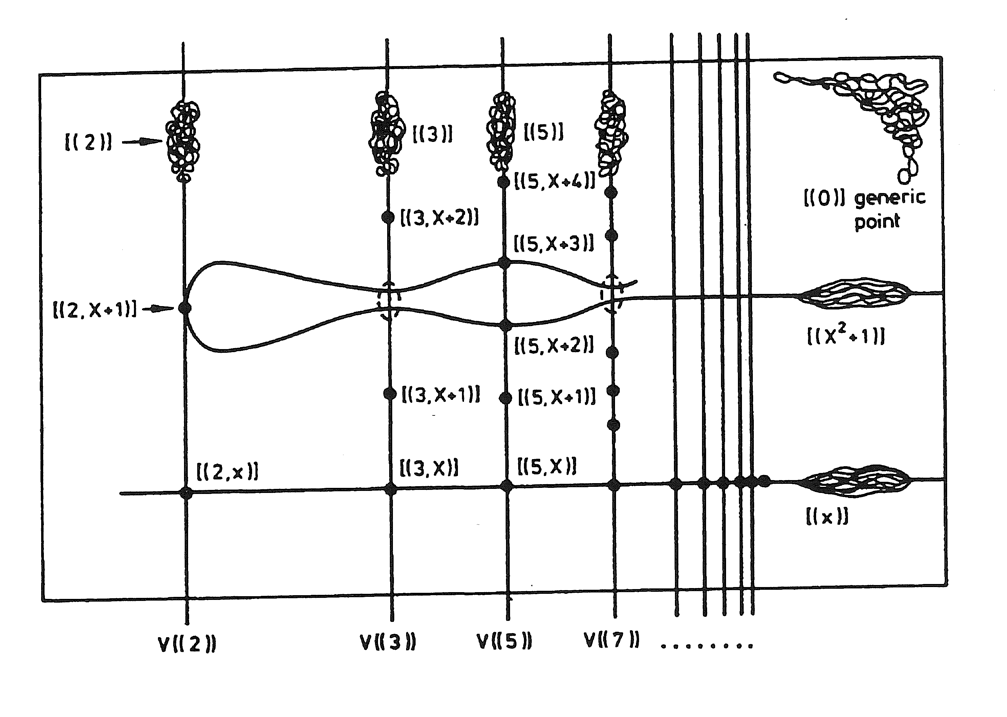
\includegraphics[width=\linewidth,height=\textheight,keepaspectratio]{Figures/Spec Z[x].png}
                                \caption{Mumford's arithmetic plane (\cite{redbook}, example II.H, pp. 75)}
                                \label{fig: integer_affine_line}
                            \end{figure}
                            \noindent
                            \begin{enumerate}
                                \item First of all, let us try to describe the points of $\A^1_{\Z}$, i.e. the prime ideals of $\Z[x]$. The upshot is that they are of the following forms:
                                    \begin{enumerate}
                                        \item $(0)$.
                                        \item $(p)$ with $p$ prime.
                                        \item $(f)$ with $f \in \Z[x]$ irreducible over $\Q$ and such that its coefficients are simultaneously coprime.
                                        \item $(p, f)$ with $p$ prime and $f \in \Z[x]$ irreducible over $\F_p$. Furthermore, these are the closed points (i.e. maximal ideals).
                                    \end{enumerate}
                                
                                \item Now, what do the fibres over $\Spec \Z$ of $\A^1_{\Z}$ look like ? Points of $\Spec \Z$ are prime ideals $\p$ of $\Z$, i.e. they are either $(0)$ or $(p)$, with $p$ some prime, and at said points, the stalks of the structure sheaf $\calO_{\Spec \Z}$ are precisely the localisations $\Z_{\p}$ (see \ref{coro: structure_sheaf_properties} for a proof). Taking the quotient of these local rings by their unique maximal ideals then shows us that the residue fields there, $\kappa_{\p}$, whose spectra consist of a single point and whose mappings into $\Spec \Z$ are precisely the identifications of prime ideals as points, are just either $\Q$ or $\F_p$ respectively. Then, by applying the duality:
                                    $$\Sch^{\aff}_{/\Spec \Z} \cong {}^{\Z/}\Comm\Alg^{\op}$$
                                it can be easily shown that the fibre of $\A^1_{\Z}$ over a point $\p$ of $\Spec \Z$ is nothing but the affine line $\A^1_{\kappa_{\p}}$. 
                            \end{enumerate}
                        \item \textbf{(Baby's second moduli space: The affine $n$-spaces over $\Z$):}
                            \begin{figure}[H]
                                \centering
                                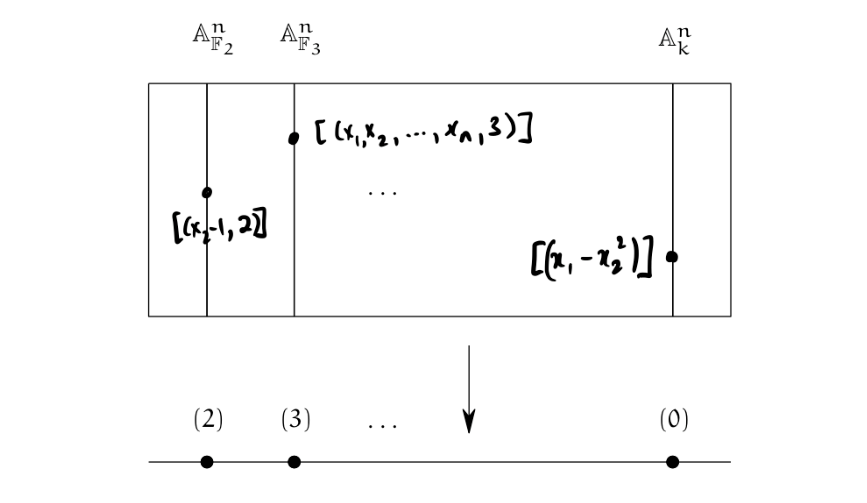
\includegraphics[width=\linewidth,height=\textheight,keepaspectratio]{Figures/affine n-space over Z.png}
                                \caption{The affine $n$-space over $\Z$ as an $\A^n$-bundle over $\Spec \Z$ (\cite{risingsea}, figure 3.7)}
                                \label{fig: affine_n_space_over_Z}
                            \end{figure} 
                        \noindent
                        By reasoning as above, it is not hard to see why the fibres over $\Spec \Z$ of $\A^n_{\Z}$ are the affine $n$-spaces $\A^n_{\kappa_{\p}}$, with $\p = (0), (p)$, as shown in the figure.
                    \end{enumerate}
                \end{example}
            
        \subsection{A zoo of topoi on \texorpdfstring{$\Cring^{\op}$}{}}
            \subsubsection{Zariski topoi} \index{Topoi!Zariski}
                \paragraph{Big and small Zariski topoi}
                    \begin{theorem}[Small Zariski topoi classify local rings]
                        Let $k$ be an arbitrary base commutativer ring. Then, the small Zariski topos $(\Spec k)^{\petit}_{\Zar}$ (cf. definition \ref{def: zariski_topoi}) is the \href{https://ncatlab.org/nlab/show/classifying+topos}{\underline{classifying topos}} for the theory of local rings.
                    \end{theorem}
                        \begin{proof}
                            
                        \end{proof}
                    
                    \paragraph{Internal locales and relative spectra} \index{Relative $\Spec$} \index{Schemes!relative affine}
                    \textit{This entry on relative affine schemes should be read after section \ref{section: schemes} on schemes, and section \ref{section: qcoh} on quasi-coherent modules. Readers who are familiar wit hthe materials therein may ignore this warning}
                    
                    So far, we have been exploring the idea that affine schemes are actually little more than objects of a category that is formally dual to some category of commutative algebras (i.e. commutative monoids within a given closed symmetric monoidal category). This while being rather powerful as a geometric characterisation of the theory of commutative rings, is somewhat lacking: particularly, the theory of affine schemes as we have been building it up, is rather local in nature. \todo{Keep writing introduction}
                    
                    \begin{definition}[Relative affine schemes] \label{def: relative_affine_schemes}
                        Let $k$ be an arbitrary base commutative ring and let $\calY$ be a base prestack on ${}^{k/}\Comm\Alg^{\op}$ (i.e. a category internal to the presheaf topos $(\Spec \Z)$). Then, let us define the category of affine schemes over $\calY$, which we shall denote by $\Sch^{\aff}_{/\calY}$, to be \textit{dual} to the subcategory ${}^{\calY/}\Comm\Alg$ of quasi-coherent commutative monoids internal to the (closed) symmetric monoidal category $\QCoh^*(\calY)$ of quasi-coherent modules on $\calY$). In notations, this reads:
                            $$\Sch^{\aff}_{/\calY} \cong {}^{\calY/}\Comm\Alg^{\op}$$
                    \end{definition}
                    \begin{remark}[Compatibility with the Yoneda-esque approach]
                        \noindent
                        \begin{enumerate}
                            \item \textbf{(Well-definiteness):} In remark \ref{remark: weak_2_yoneda}, we gave an alternate definition of what it means for a prestack on $\Cring^{\op}$ to be an affine scheme over other given base prestack: they are just objects of a certain slice category. But does this formulation agree with that of definition \ref{def: relative_affine_schemes} ? 
                        
                            Suppose that we are working over a base prestack $\calY$. First of all, note that objects of $\Sch^{\aff}_{/\calY}$, i.e. affine schemes over $\calY$, are presheaves on $\Cring^{\op}$ themselves, as the category ${}^{\calY/}\Comm\Alg$ of quasi-coherent commutative monoids internal to the symmetric monoidal category of quasi-coherent modules on $\calY$
                            \item \textbf{(These all seem awfully abstract ...):} Relative affine schemes should best (at least in the opinion of the author) be thought of as objects of categories that are fibres parametrised by the $1$-category $[\Spec \Z]$ of prestacks over $\Cring^{\op}$: that is, one should think of categories of relative affine schemes as coming from a prestack:
                                $$\Sch^{\aff}_{/(-)}: [\Spec \Z]^{\op} \to \Cat$$
                            This might seem like a rather pointless abstraction, or to put it even more critically, just an abstraction for the sake of abstraction. However, its virtue lies in how the fibres over objects of $[\Spec \Z]$ that happen to be affine schemes $\Spec k$ (in the sense of definition \ref{def: zariski_topoi}) would just be the categories $\Sch^{\aff}_{/\Spec k}$, which we have a rather solid handle on. This, incidentally, suggests a remarkable idea: there is a more-or-less functorial way to realise the idea that prestacks are locally affine. In fact, we shall return to this abstraction and analyse it in more details in proposition \ref{prop: relative_Spec_on_schemes}, where we will see how the domain restriction $\Sch^{\aff}_{/(-)}|_{\Sch}$ of the prestack $\Sch^{\aff}_{/(-)}$ to $\Sch$ instead of $[\Spec \Z]$ is actually stack on $\Sch_{\Zar}$.
                        \end{enumerate}
                    \end{remark}
                    
                    \begin{proposition}[Relative $\Spec$ on schemes] \label{prop: relative_Spec_on_schemes}
                        Let $S$ be a base scheme. Then, the prestack of relative affine schemes:
                            $$\Sch^{\aff}_{/(-)}|_{\Sch_{/S}}: \Sch_{/S}^{\op} \to \Cat$$
                        is a stack on $\Sch_{/S, \Zar}$ (which should be intuitively true, since schemes are covered by affines after all).
                    \end{proposition}
                        \begin{proof}
                            
                        \end{proof}
                
            \subsubsection{\'Etale topoi} \index{Topoi!\'etale}
            
            \subsubsection{Fppf topoi} \index{Topoi!fppf}
        
    \section{Schemes} \label{section: schemes}
        \begin{convention}[\textcolor{red}{\underline{\textbf{IMPORTANT}}} Prestacks and stacks] \label{conv: prestacks} \index{Prestacks} \index{Stacks}
            \noindent
            \begin{enumerate}
                \item \textbf{(The descent-theoretic perspective):} \begin{enumerate}
                    \item \textbf{(Prestacks):} To us, a \textbf{prestack} on a $1$-category $\C$ will always be a \textit{weak} $2$-functor (i.e. a $2$-functor that respects compositions only up to natural isomorphisms) from $\C^{\op}$ (viewed as a tautological weak $2$-category) into the \href{https://ncatlab.org/nlab/show/bicategory}{\underline{weak $2$-category}} ${}^1\Cat$ of small $1$-categories, (ana)functors between them, and (ana-)natural transformations between these (ana-)functors (see definition \ref{def: internal_functors} for the definition of anafunctors, along with an explanation of why this is our chosen definition of ${}^1\Cat$). In other terminologies, a prestack is a \href{https://ncatlab.org/nlab/show/pseudofunctor}{\underline{pseudo-functor}} with values in ${}^1\Cat$. Prestacks over a given category $\C$ form a $1$-category in an obvious manner; we shall denote it by $\Pre\Stk(\C)$. Actually, for all base categories $\C$, the $1$-category $\Pre\Stk(\C)$ can also be endowed with the structure of a weak $2$-category, determined on the $2$-categorical level by $2$-morphisms which are \href{https://ncatlab.org/nlab/show/strict+2-natural+transformation}{\underline{\textit{strict} $2$-natural transformations}}.
                    
                    Additionally, we shall assume the Axiom of Choice (which incidentally, forces us to adopt definition \ref{def: internal_categories}). The advantage in this is that for all base categories $\C$, we will automatically be given a \textit{weak} $2$-equivalence of \textit{weak} $2$-categories:
                        $$\Pre\Stk(\C) \cong \Fib(\C)$$
                    between the weak $2$-category of prestacks on $\C$ and that of fibred categories on $\C$ (see subsection 3.1.3 of \cite{vistoli_descent} for a proof). Logicians might scoff at such a practice, but since choosing cleavages in algebraic geometry is mostly just asking for trouble, we shall try to bear the shame of having Choice.
                    \item \textbf{(Stacks):} Let us build upon the above notion of prestacks and declare that throughout this book, the term \say{\textbf{stack}} shall mean \say{sheaf of categories}, i.e. a stack is a fibred category which satisfies descent; concretely, a stack $\calX$ over a site $(\C, J)$ is a prestack such that for all objects $X$ of $\C$ and all covering $J$-sieves $\U_{/X}$ thereon, one has the following equivalence of categories:
                        $$\calX(X) \cong \calX\left(\underset{U \in \U_{/X}}{\colim} h_U\right)$$
                    Stacks on $(\C, J)$ form a full weak $2$-subcategory of the weak $2$-category $\Pre\Stk(\C)$ of prestacks on $\C$, which shall be denoted by $\Stk(\C, J)$. Furthermore, stacks of groupoids (i.e. categories fibred in groupoids that satisfy descent) on small sites $(\C, J)$ form a \href{https://ncatlab.org/nlab/show/(n,1)-topos}{\underline{$(2, 1)$-topos}} which is written $\Sh_{(2,1)}(\C, J)$; occasionally, we might refer to these as sheaves of groupoids; naturally, $\Sh_{(2,1)}(\C, J)$ comes equipped with a \href{https://ncatlab.org/nlab/show/adjoint+\%28infinity\%2C1\%29-functor}{\underline{$(2, 1)$-geometric embedding}} into the weak $2$-category $\Psh_{(2, 1)}(\C)$ of prestacks of groupoids on $\C$.
                \end{enumerate}
                We refer the reader to \cite{vistoli_descent} for an exposition to prestacks and stacks (in the above senses) that can hardly improved upon. \cite{riehl_loregian_fibration} may also be used as a supplementary reference for the topics of \href{https://ncatlab.org/nlab/show/Grothendieck+fibration#definition}{\underline{fibration}} and \href{https://ncatlab.org/nlab/show/Grothendieck+construction}{\underline{the Grothendieck construction}}. Finally, we have our own appendix on fibred categories; cf. section \ref{section: moduli_problems}.
                \item \textbf{(The internal point of view):} From the internal point of view (which in the opinion of the author, is a lot more intuitive; this is, however, purely personal), (pre)stacks (respectively $(2, 1)$-(pre)sheaves) are nothing but internal categories (respectively internal groupoids) inside (pre)sheaf topoi.
            
                Readers may also have heard of mysterious entities known as \textbf{gerbes}. There are many definitions floating around, but again, let us fix one meaning for the term. To us, a gerbe on a site $(\C, J)$ will always be group internal to $\Stk(\C, J)$ (i.e. a sheaf of strict $2$-groups \cite{nlab:strict_2-group}, or in other words, an internal groupoid in $\Sh_{\Sets}(\C, J)$ whose object of objects is the terminal object of $\Sh_{\Sets}(\C, J)$). Additionally, should there be no non-trivial automorphisms, the notion of gerbes shall reduce to that of principal bundles. We refer the reader to the discussions in \href{https://mathoverflow.net/questions/263832/phenomena-of-gerbes}{\underline{this MathOverflow thread}} for examples of gerbes. 
            \end{enumerate}
        \end{convention}
        
        \begin{remark}[Affine schemes over general (pre)stacks] \label{remark: weak_2_yoneda}
            Once more has Yoneda come to our rescue, albeit this time, along with his twin brother (yes I am fully prepared for a punishment fit for that crime of a joke): it's \href{https://ncatlab.org/nlab/show/Yoneda+lemma+for+bicategories}{\underline{the weak $2$-Yoneda lemma}}. Essentially, instead of embedding a base category $\C$ into the $1$-category of presheaves of sets $\Psh_{\Sets}(\C)$ thereon, we shall be viewing $\C$ as a tautological weak $2$-category, and shall instead be embedding it into the weak $2$-category $\Pre\Stk(\C)$ of prestacks/pseudo-functors over $\C$ via a \href{https://ncatlab.org/nlab/show/full+sub-2-category}{\underline{fully faithful $2$-functor}}, known as the $2$-Yoneda embedding. Via the $2$-Yoneda embedding, one can view objects of $\C$ as prestacks fibred in sets (which we note to be $2$-categories wherein all $1$-cells and $2$-cells are identities), and therefore, the notion of objects of $\C$ with mappings into a arbitrarily given base prestack $\calY \in \Pre\Stk(\C)$ is well-defined; in particular, one can meaningfully talk about affine schemes over prestacks on $\Cring^{\op}$. 
            \\
            For a detailed discussion of the weak $2$-Yoneda embedding, the reader may consult \cite{nlab:yoneda_lemma_for_bicategories}.
        \end{remark}
        
        \begin{example}[Punctured prestacks] \label{example: punctured_prestacks}
            Let $R$ be any commutative ring and let $\p$ be a prime ideal thereof, and let us make no distinction between $\p$ and the corresponding point in $|\Spec R|$. Now, to begin, let us recall that the localisation $R_{\p}$ of $R$ at $\p$ is a local ring whose \textit{unique} maximal ideal is precisely $\p R_{\p}$ (cf. corollary \ref{coro: localisation_at_primes}): in particular, this means that there is a bijective correspondence between prime ideals of $R$ (i.e. points of $|\Spec R|$) and localisations of $R$ at these primes. This means, that the \textit{canonical} morphism of affine schemes:
                $$\Spec R_{\p} \to \Spec R$$
            gives us an identification of the point $\p$ inside $|\Spec R|$ (usually, one would consider the morphism $\Spec \kappa_{\p} \to \Spec R$ instead, as spectra of fields are actually singleton spaces). Alternatively, this morphism might be thought of as the identification of the open subscheme $\Spec R_{\p}$ inside $\Spec R$, whose underlying topological space we note to precisely be the complement $|\Spec R| \setminus \{\p\}$. Thus, we have managed to puncture the affine scheme $\Spec R$ at $\p \in |\Spec R|$. 
            
            On the surface, this might seem like nothing more than a fun observation, but in fact, it is a rather powerful one. The fact that a \textit{canonical} morphism helps us puncture an affine scheme at a given point means that we can perform a similar procedure on general prestacks on $\Cring^{\op}$ and do not have to restrict ourselves to affine schemes. The way that we shall be going about this is as follows: if we are to consider the category $\Sch^{\aff}_{/\calY}$ of affine schemes over some given base prestack $\calY \in [\Spec \Z]$, then we can define the prestack $\calY^{\circ}$ (or $\calY^{\circ}_{\p}$ when the choice of $\p$ is not obvious) that is punctured at $\p \in |\Spec R|$ (for some $\Spec R \in \Sch^{\aff}_{/\calY}$) to be that specified by the following condition:
                $$\calY^{\circ}(\Spec R) \cong \calY(\Spec R_{\p})$$
            and thanks to the fact that there is a canonical morphism in $\Cring^{\op}$ from $\Spec R_{\p}$ to $\Spec R$, there is a canonical morphism from $\calY(\Spec R)$ to $\calY(\Spec R_{\p})$, or equivalently, a pseudo-natural transformation:
                $$\calY \to \calY^{\circ}$$
            Any prestack satisfying these specifications shall be known as a \textbf{punctured prestack}. 
            
            But hold on, was it just not asserted that it is a morphism from $\Spec R_{\p}$ to $\Spec R$, not the other way around, that identifies the puncturing of $\Spec R$ at $\p$ ? Well, in this case - and all other cases of affine schemes for that matter - one must view this canonical arrow as the input of the representable prestack $\Cring^{\op}(-, \Spec R)$, which is often abbreviated by $h_{\Spec R}$. Then, one gets that:
                $$h_{\Spec R}^{\circ}(\Spec R) \cong h_{\Spec R}(\Spec R_{\p})$$
            which gives us the \say{correct} arrow:
                $$h_{\Spec R} \to h_{\Spec R}^{\circ}$$
            via the canonical arrow $h_{\Spec R}(\Spec R) \to h_{\Spec R}(\Spec R_{\p})$. 
        \end{example}
        
        \begin{example}[Multi-punctured prestacks] \label{example: multi_punctured_prestacks}
        
        \end{example}
        
        \begin{example}[Arcs and loops] \label{example: arcs_and_loops}
            The \textbf{arc space} or \textbf{$\infty$-jet space/bundle} associated to a prestack $\calY$ on $\Cring^{\op}$ is a prestack $\calY[\![t]\!]$ given by:
                $$\calY[\![t]\!](\Spec R) \cong \calY(\Spec R [\![t]\!])$$
            for all objects $\Spec R$ of $\Cring^{\op}$ and some variable $t$ that is transcendental over $R$; there might also come times when we would like to emphasise how $\calY[\![t]\!]$ is like the space of formal Taylor series over $\calY$, and in those cases, we shall write $\Jet^{\infty}\calY$ instead of $\calY[\![t]\!]$. In a similar fashion, the \textbf{loop space} associated to $\calY$, denoted by $\calY (\!(t)\!)$, is the prestack given by:
                $$\calY(\!(t)\!)(\Spec R) \cong \calY(\Spec R (\!(t)\!))$$
                
            One can also define lower-dimensional jets; for each natural number $n$, the space of $n$-jets on $\calY$ is a prestack $\Jet^n\calY$ which is given by:
                $$\Jet^n\calY(\Spec R) \cong \calY(\Spec R[t]/t^{n + 1})$$
        \end{example}
    
        \subsection{Schemes are geometric stacks}
            \subsubsection{Principal bundles in algebraic geometry}
                \paragraph{\textit{Pr\'elude}: Internal categories and equivalence relations therein}
                    We shall be defining quotient stacks using the language of internal groupoids, which shall be defined below via the more general notion of internal categories. This is a rather high-tech approach, but it is superior to other (more traditional) approaches in that what equivalence relations - particularly those induced by group actions - can now be understood rather syntactically.
                
                    \begin{definition}[Internal categories] \label{def: internal_categories}
                        Let $\E$ be a category with \textit{enough pullbacks}. A category \textbf{internal} to $\E$ is then a pair $(C_0, C_1)$ of objects of $\E$ defined via the following data:
                            \begin{enumerate}
                                \item \textbf{(Objects and morphisms):} An object of \textbf{objects} $C_0 \in \E$ and an object of \textbf{arrows} $C_1 \in \E$, both are to be viewed as internal analogues of the collections of objects and arrows in the definition of categories.
                                \item \textbf{(Composition):} 
                                    \begin{enumerate}
                                        \item \textbf{(Sources and targets):} From the object of arrows $C_1$ to the object of objects $C_0$, there are two morphisms $s, t$ as follows, known as the \textbf{source} and \textbf{target} maps:
                                            $$
                                                \begin{tikzcd}
                                                	{C_1} & {C_0}
                                                	\arrow["s", shift left=2, from=1-1, to=1-2]
                                                	\arrow["t"', shift right=2, from=1-1, to=1-2]
                                                \end{tikzcd}
                                            $$
                                        which, respectively, assign to each arrow $f \in C_1$ (which, along with similar instances, shall be viewed as a \href{https://ncatlab.org/nlab/show/generalized+element}{\underline{generalised elements}} for the sake of linguistic convenience) its domain and codomain objects in $C_0$.
                                        \item \textbf{(Units):} From the object of objects $C_0$ to the object of arrows $C_1$, there is a distinguished morphism:
                                            $$e: C_0 \to C_1$$
                                        called the \textbf{unit map} which assigns to each object $x \in C_0$ (again, viewed as a generalised element) the identity $\id_x: x \to x$ thereon, which we note to be an a generalised element of the object of arrows $C_1$ (hence the codomain of $e$ is $C_1$).
                                        \item \textbf{(Composition of arrows):} There is a monoidal composition operation (in the sense of monoidal categories):
                                            $$\mu: C_1 \x_{s, C_0, t} C_1 \to C_1$$
                                        satisfying the following conditions specified by commutative diagrams in $\E$:
                                            \begin{enumerate}
                                                \item \textbf{(Identities do not alter domains and codomains):}
                                                    $$
                                                        \begin{tikzcd}
                                                        	{C_0} & {C_1} && {C_0} & {C_1} \\
                                                        	& {C_0} &&& {C_0}
                                                        	\arrow["e", from=1-1, to=1-2]
                                                        	\arrow["{\id_{C_0}}"', from=1-1, to=2-2]
                                                        	\arrow["s", from=1-2, to=2-2]
                                                        	\arrow["{\id_{C_0}}"', from=1-4, to=2-5]
                                                        	\arrow["t", from=1-5, to=2-5]
                                                        	\arrow["e", from=1-4, to=1-5]
                                                        \end{tikzcd}
                                                    $$
                                                \item \textbf{(Sources and targets of compositions):} The source of a composition $g \mu f \in C_1$ should be that of $f$ (the former), wheareas its target should be that of $g$ (the latter): 
                                                    $$
                                                        \begin{tikzcd}
                                                        	& {C_1 \x_{s, C_0, t} C_1} & {C_1} && {C_1 \x_{s, C_0, t} C_1} & {C_1} \\
                                                        	{} & {C_1} & {C_0} && {C_1} & {C_0}
                                                        	\arrow["s", from=1-3, to=2-3]
                                                        	\arrow["s", from=2-2, to=2-3]
                                                        	\arrow["{\pr_2}"', from=1-2, to=2-2]
                                                        	\arrow["{\pr_1}", from=1-2, to=1-3]
                                                        	\arrow["t", from=1-6, to=2-6]
                                                        	\arrow["t", from=2-5, to=2-6]
                                                        	\arrow["{\pr_1}"', from=1-5, to=2-5]
                                                        	\arrow["{\pr_1}", from=1-5, to=1-6]
                                                        \end{tikzcd}
                                                    $$
                                                \item \textbf{(Associativity):} 
                                                    $$
                                                        \begin{tikzcd}
                                                        	& {C_1 \x_{s, C_0, t} C_1 \x_{s, C_0, t} C_1} & {C_1 \x_{s, C_0, t} C_1} \\
                                                        	{} & {C_1 \x_{s, C_0, t} C_1} & {C_1}
                                                        	\arrow["\mu", from=1-3, to=2-3]
                                                        	\arrow["\mu", from=2-2, to=2-3]
                                                        	\arrow["{\id_{C_1} \x_{s, C_0, t} \mu}"', from=1-2, to=2-2]
                                                        	\arrow["{\mu \x_{s, C_0, t} \id_{C_1}}", from=1-2, to=1-3]
                                                        \end{tikzcd}
                                                    $$
                                                \item \textbf{(Left and right-unitarity):} 
                                            \end{enumerate}
                                                $$
                                                    \begin{tikzcd}
                                                    	{C_0 \x_{C_0} C_1} & {C_1 \x_{s, C_0, t} C_1} & {C_1 \x_{C_0} C_0} \\
                                                    	& {C_1}
                                                    	\arrow["\mu", from=1-2, to=2-2]
                                                    	\arrow["{\pr_2}"', from=1-1, to=2-2]
                                                    	\arrow["{\pr_1}", from=1-3, to=2-2]
                                                    	\arrow["{\e \x_{C_0} \id_{C_1}}", from=1-1, to=1-2]
                                                    	\arrow["{\id_{C_1} \x_{C_0} e}"', from=1-3, to=1-2]
                                                    \end{tikzcd}
                                                $$
                                        with the latter three specifying the monoidality of the composition operation $\mu$.
                                    \end{enumerate}
                            \end{enumerate}
                    \end{definition}
                    
                    \begin{remark}[Internal categories vs. subcategories]
                            
                    \end{remark}
                    
                    \begin{remark}[Another formulation: Internal categories as monads on spans] \label{remark: internal_categories_alt_def}
                        Definition \ref{def: internal_categories} gives us a perfectly fine idea of what one might mean by \say{internal categories}. However, it is manifestly rather clunky. Therefore, the author has taken the liberty to provide one alternative formulation of the notion of internal categories.
                        
                        We refer the reader to definition \ref{def: spans} and the discussion that follows for necessary information on the paradigm of spans; in particular, let us recall that spans are only well-defined inside categories with pullbacks (which is a slightly stronger condition than the assumption in definition \ref{def: internal_categories} that the ambient category as merely \textit{enough} pullbacks). 
                            
                        Now, let $\E$ be an ambient category with all pullbacks, and subsequently, let us define a category $C$ internal to $\E$ as being the same as a monad in the weak $2$-category $\Span^{\leq 2}(\E)$ of spans on $\E$. Why would this even resemble a reasonable definition of categories internal to a given category $\E$ ? For starters, recall that a monad is an endomorphism satisfying so-called \say{monoidal multiplication}. Therefore, an internal category $C$ inside a given ambient category $\E$ is first and foremost an endomorphism on a choice of object, and because the weak $2$-category in which we are trying to build monads is one of spans, our endomorphism should be a \say{roof} diagram whose two \say{lower} vertices are the same. By consulting definition \ref{def: internal_categories}, one sees that an obvious choice is the source-target span:
                            $$
                                \begin{tikzcd}
                                	{C_1} & {C_0} \\
                                	{C_0}
                                	\arrow["s"', from=1-1, to=2-1]
                                	\arrow["t", from=1-1, to=1-2]
                                \end{tikzcd}
                            $$
                        (recall that objects in span categories are those of the underlying category and morphisms are span themselves; cf. definition \ref{def: spans}); let us denote this span by the \textit{unordered} pair $(s, t)$. Now, is this endomorphism indeed a monad in $\Span^{\leq 2}(\E)$ ? First of all, one can certainly compose $(s, t)$ with itself thanks to the assumption that $\E$ has all pullbacks: said composition is nothing but the composite span $(s, t) \x (s, t)$ (see remark \ref{conv: span_notations} for an explanation of this notation); let us denote this composition by $\mu$, and note that it is precisely a $2$-cell from $(s, t) \x (s, t)$ to $(s, t)$, a fact that can be proven via consideration of the following universal diagram:
                            $$
                                \begin{tikzcd}
                                	{(s, t) \x (s, t)} & {(s, t)} \\
                                	{(s, t)} & {(s, t)}
                                	\arrow[dashed, from=1-1, to=2-1]
                                	\arrow[dashed, from=1-1, to=1-2]
                                	\arrow[Rightarrow, no head, from=1-2, to=2-2]
                                	\arrow[Rightarrow, no head, from=2-1, to=2-2]
                                	\arrow["\mu", from=1-1, to=2-2]
                                \end{tikzcd}
                            $$
                        and thanks to the universal property of products, this composition is trivially asociative. There is also a unit $e := (\id_{C_0}, \id_{C_0}) \x (s, t)$ which satisfies the following commutative diagram:
                            $$
                                \begin{tikzcd}
                                	{(\id_{C_0}, \id_{C_0}) \x (s, t)} & {(s, t) \x (s, t)} & {(s, t) \x (\id_{C_0}, \id_{C_0})} \\
                                	& {(s, t)}
                                	\arrow["\mu", from=1-2, to=2-2]
                                	\arrow["{\pr_2}"', from=1-1, to=2-2]
                                	\arrow["{\pr_1}", from=1-3, to=2-2]
                                	\arrow["{e \x \id_{(s, t)}}", from=1-1, to=1-2]
                                	\arrow["{\id_{(s, t)} \x e}"', from=1-3, to=1-2]
                                \end{tikzcd}
                            $$
                        This proves that the composition $\mu$ is also unital, and hence all the monad axioms have been shown to hold. Incidentally, we have also managed to show via this discussion, that monads in the category of spans in a category with pullbacks are nothing but internal categories.
                    \end{remark}
                    
                    \begin{definition}[Internal functors] \label{def: internal_functors}
                        Let $\E$ be an ambient category with \textit{enough pullbacks} and let $C, D$ be two categories that are internal to $\E$.
                            \begin{enumerate}
                                \item \textbf{(Internal functors):} Internal functors between categories that are internal to a given ambient category (with enough pullbacks) are defined in the exact same way as the internal definition of functors between ordinary categories. See \href{https://ncatlab.org/nlab/show/functor#InternalDefinition}{\underline{here}} for a reminder.
                                \item \textbf{(Anafunctors):} (Ah yes, the Axiom of Choice. Making lives miserable as always) While the general definition of internal functors might not have lit any bulbs in the deparment of choice, one should definitely keep in mind that the notion of essential surjectivity definitely does depend on choice: if:
                                    $$F: C \to D$$
                                is an essentially surjective internal functor, then one will be able to \textit{choose} objects $x \in C_0$ such that:
                                    $$Fx \cong y$$
                                for every object $y \in D_0$. As the ramifications of the Axiom of Choice tend to be unfamiliar to those not actively involved in the logic community (including the author, who had to go read a few \textcolor{ForestGreen}{nLab} too), let us quickly explain why anafunctors are needed in place of the above \textit{na\"ive} notion of internal functors; particularly, we would like to know what mappings between internal categories might look like when our ambient category does not host the Axiom of Choice, such as when its size is an inaccessible cardinal ($\Top$ is one particular case). To that end, \todo{Write about why the Axiom of Choice breaks essentially surjective internal functors}
                                
                                Now, let us define an \textbf{anafunctor} $F$ between two internal categories $C$ and $D$ of a given category $\E$ - should such a mapping exist - to be a span (i.e. a $1$-morphism in $\Span^{\leq 2}(\E)$; cf. definition \ref{def: spans}) of internal categories:
                                    $$
                                        \begin{tikzcd}
                                        	{F} & {D} \\
                                        	{C}
                                        	\arrow[from=1-1, to=2-1]
                                        	\arrow[from=1-1, to=1-2]
                                        \end{tikzcd}
                                    $$
                                which shall be interpreted as the following composition of spans in $\E$:
                                    $$
                                        \begin{tikzcd}
                                        	\bullet & \bullet & {D_1} & {D_0} \\
                                        	\bullet & {F_0} & {D_0} \\
                                        	{C_1} & {C_0} \\
                                        	{C_0}
                                        	\arrow[from=3-1, to=4-1]
                                        	\arrow[from=3-1, to=3-2]
                                        	\arrow[from=2-2, to=3-2]
                                        	\arrow[from=2-2, to=2-3]
                                        	\arrow[from=1-3, to=2-3]
                                        	\arrow[from=1-3, to=1-4]
                                        	\arrow[from=2-1, to=3-1]
                                        	\arrow[from=2-1, to=2-2]
                                        	\arrow[from=1-1, to=2-1]
                                        	\arrow[from=1-1, to=1-2]
                                        	\arrow[from=1-2, to=2-2]
                                        	\arrow[from=1-2, to=1-3]
                                        	\arrow["\lrcorner"{anchor=center, pos=0.125}, draw=none, from=1-2, to=2-3]
                                        	\arrow["\lrcorner"{anchor=center, pos=0.125}, draw=none, from=1-1, to=2-2]
                                        	\arrow["\lrcorner"{anchor=center, pos=0.125}, draw=none, from=2-1, to=3-2]
                                        \end{tikzcd}
                                    $$
                                (see remark \ref{remark: internal_categories_alt_def} for a description of internal categories as spans - or to be more precise, monads in span categories). Note that in the event that $\E$ also has products (or equivalently, terminal objects), anafunctors between any given pair of internal categories $C$ and $D$ always exist: one can simply take $F_0$ to be $C_0 \x D_0$. Also, let us draw attention to the fact that this definition is logically independent of the notion of internal functors, and therefore we have not committed circular reasoning.
                            \end{enumerate}
                    \end{definition}
                    \begin{remark}[Categories of internal categories] \label{remark: categories_of_internal_categories}
                        Via the above notion of anafunctors and the idea presented in remark \ref{remark: internal_categories_alt_def} that internal categories and monads in span categories are the same thing, one can rather easily show that categories internal to a given ambient category $\E$ (with pullbacks) form a weak $2$-category, which is precisely equivalent to the category of monads in $\Span^{\leq 2}(\E)$. In notations, one writes:
                            $$\Cat(\E) \cong \Monad\left(\Span^{\leq 2}(\E)\right)$$
                    \end{remark}
                    \begin{remark}[Categories as monoids] \label{remark: categories_as_monoids}
                        Remark \ref{remark: internal_categories_alt_def}, definition \ref{def: internal_functors}, remark \ref{remark: categories_of_internal_categories}, and remark \ref{conv: span_notations} in tandem tell us that internal to every ambient category $\E$ with pullbacks, there is a symmetric monoidal category $\Cat(\E)$ of categories internal to $\E$ whose monoidal multiplication is given by $2$-spans from squares:
                            $$
                                \begin{tikzcd}
                                	{C_1 \x_{s, C_0, t} C_1} \\
                                	& {C_1} & {C_0} \\
                                	& {C_0}
                                	\arrow["s", from=2-2, to=3-2]
                                	\arrow["t"', from=2-2, to=2-3]
                                	\arrow[from=1-1, to=3-2]
                                	\arrow[from=1-1, to=2-3]
                                	\arrow["\mu"{description}, from=1-1, to=2-2]
                                \end{tikzcd}
                            $$
                        and whose monoidal unit is given pointwise on each internal category:
                            $$
                                \begin{tikzcd}
                                	{C_1} & {C_0} \\
                                	{C_0}
                                	\arrow["s"', from=1-1, to=2-1]
                                	\arrow["t", from=1-1, to=1-2]
                                \end{tikzcd}
                            $$
                        by a $2$-span from $(\id_{C_0}, \id_{C_0}) \to (s,t)$:
                            $$
                                \begin{tikzcd}
                                	{C_0} \\
                                	& {C_1} & {C_0} \\
                                	& {C_0}
                                	\arrow["s", from=2-2, to=3-2]
                                	\arrow["t"', from=2-2, to=2-3]
                                	\arrow["e"{description}, from=1-1, to=2-2]
                                	\arrow["{\id_{C_0}}"', from=1-1, to=3-2]
                                	\arrow["{\id_{C_0}}", from=1-1, to=2-3]
                                \end{tikzcd}
                            $$
                        Both of which (together) are subjected to the usual monoidal axioms (cf. definition \ref{def: internal_categories}). In other words, internal categories inside a given ambient category $\E$ are nothing but monoids in $\Cat(\E)$. This is a rather neat observation, as it allows us to view morphisms between internal categories not too differently from monoid homomorphism. 
                    \end{remark}
                    
                    \begin{example}[Examples of internal categories] \label{example: internal_categories}
                        \noindent
                        \begin{enumerate}
                            \item \textbf{(Categories):} Every small $1$-category is internal to $\Sets$.
                            \item \textbf{($\omega$-categories and $n$-categories):} 
                            \item \textbf{(Prestacks and stacks):} A category internal to the category of presheaves on a given base category is a prestack, and a category internal to the sheaf topos on a given base site is a stack. In particular, groupoids internal to (pre)sheaf topoi are (pre)stacks of groupoids (see definition \ref{def: internal_groupoids} and example \ref{example: internal_groupoids_and_equivalence_relations} for more details on internal groupoids).  
                        \end{enumerate}
                    \end{example}
                    
                    \begin{definition}[Internal groupoids] \label{def: internal_groupoids}
                        Let $\E$ be a category with pullbacks and let:
                            $$
                                \begin{tikzcd}
                                	{\scrG_1} & {\scrG_0} \\
                                	{\scrG_0}
                                	\arrow["s"', from=1-1, to=2-1]
                                	\arrow["t", from=1-1, to=1-2]
                                \end{tikzcd}
                            $$
                        be the data of a category internal to $\E$. Such an internal category is an \textbf{internal groupoid} if in addition, there exists an arrow:
                            $$i: \scrG_1 \to \scrG_1$$
                        called the \textbf{inverse map}, that renders the following diagram in $\E$ commutative:
                            $$
                                \begin{tikzcd}
                                	{\scrG_1} \\
                                	& {\scrG_1} & {\scrG_0} \\
                                	& {\scrG_0}
                                	\arrow["i"{description}, from=1-1, to=2-2]
                                	\arrow["t"', from=1-1, to=3-2]
                                	\arrow["s", from=2-2, to=3-2]
                                	\arrow["t"', from=2-2, to=2-3]
                                	\arrow["s", from=1-1, to=2-3]
                                \end{tikzcd}
                            $$
                        (i.e. the inverse map switches the source and target of a given internal morphism), and such that the following diagrams of spans - telling us that multiplication with inverses returns the identity regardless of whether the process is carried out from the left and from the right - commute:
                            $$
                                \begin{tikzcd}
                                	{\scrG_1} & {\scrG_1 \x_{s, \scrG_0, t} \scrG_1} & {\scrG_1 \x_{s, \scrG_0, t} \scrG_1} \\
                                	{\scrG_0} && {\scrG_1}
                                	\arrow["{\mu_{\scrG}}", from=1-3, to=2-3]
                                	\arrow["{i \x_{s, \scrG_0, t} \id_{\scrG_1}}", from=1-2, to=1-3]
                                	\arrow["{\Delta_{\scrG_1/\scrG_0}}", from=1-1, to=1-2]
                                	\arrow["t"', from=1-1, to=2-1]
                                	\arrow["e", from=2-1, to=2-3]
                                \end{tikzcd}
                            $$
                            $$
                                \begin{tikzcd}
                                	{\scrG_1} & {\scrG_1 \x_{s, \scrG_0, t} \scrG_1} & {\scrG_1 \x_{s, \scrG_0, t} \scrG_1} \\
                                	{\scrG_0} && {\scrG_1}
                                	\arrow["{\mu_{\scrG}}", from=1-3, to=2-3]
                                	\arrow["{\id_{\scrG_1} \x_{s, \scrG_0, t} i}", from=1-2, to=1-3]
                                	\arrow["{\Delta_{\scrG_1/\scrG_0}}", from=1-1, to=1-2]
                                	\arrow["s"', from=1-1, to=2-1]
                                	\arrow["e", from=2-1, to=2-3]
                                \end{tikzcd}
                            $$
                        In other words, groupoids internal to a category with pullbacks $\E$ are group objects in the category $\Cat(\E)$ of categories internal to $\E$ (which we note to have all finite products; cf. remark \ref{conv: span_notations}).
                    \end{definition}
                    \begin{remark}[On the inverse maps of internal groupoids]
                        Definition \ref{def: internal_groupoids}, while standard, suffers from a few issues. For one, it is not very clear how internal groupoids should be thought of as groups in categories of internal categories. Also, the inverse map defining the structure of each internal groupoid, at least according to definition \ref{def: internal_groupoids}, is rather non-functorial. Luckily, these two problems can be easily resolved. 
                        
                        Firstly, let us note that the inverse map $i_{\scrG}: \scrG_1 \to \scrG_1$ associated to an internal groupoid:
                            $$
                                \begin{tikzcd}
                                	{\scrG_1} & {\scrG_0} \\
                                	{\scrG_0}
                                	\arrow["s"', from=1-1, to=2-1]
                                	\arrow["t", from=1-1, to=1-2]
                                \end{tikzcd}
                            $$
                        is not just a morphism in the ambient category satisfying certain conditions, but actually a $2$-span: it is a $2$-span from the $1$-span $(s,t): \scrG_1 \toto \scrG_0$ to the $1$-span $(t,s): \scrG_1 \toto \scrG_0$. Thus, one can meaningfully think of the inverse map on $\scrG$ as an anafunctor from $\scrG$ to itself. Second of all, recall that in remark \ref{remark: categories_as_monoids}, we have seen how internal categories are actually monoid objects, which in particular, means that composition of arrows therein behaves in a manner similar to multiplication. So actually, all that we need to do is to somehow configure inverse maps so that they would act like multiplicative inverses, which would in turn help us formally recognise internal groupoids as group objects; we shall leave the drawing of the relevant commutative diagrams to the reader, as they can be rather easily inferred from the ones in definition \ref{def: internal_groupoids}. 
                    \end{remark}
                
                    \begin{definition}[Equivalence relations] \label{def: equivalence_relations}
                        Let $\E$ be a \textit{finitely complete} category ($\Sets$ or general topoi, or $\Cat$, for instance)
                            \begin{enumerate}
                                \item \textbf{(Binary relations):} A \textbf{binary relation} $R$ from an object $X$ to another object $Y$ of $\E$ is a $1$-span:
                                    $$
                                        \begin{tikzcd}
                                        	R & Y \\
                                        	X
                                        	\arrow[from=1-1, to=2-1]
                                        	\arrow[from=1-1, to=1-2]
                                        \end{tikzcd}
                                    $$
                                such that $R$ is a subobject of $X \x Y$. 
                                \item \textbf{(Equivalence relations):} An \textbf{equivalence relation} (also known as a congruence) $R$ on an object $X$ of $\E$ is a binary relation from $X$ to itself which also happens to be an internal groupoid. 
                                \item \textbf{(Quotients):} The coequaliser of an (internal) equivalence relation is known as a \textbf{quotient object}. That is, the quotient $Q$ of an object $X$ by an equivalence relation $R$ is the following coequaliser in $\E$:
                                    $$
                                        \begin{tikzcd}
                                        	R & X & Q
                                        	\arrow["s", shift left=2, from=1-1, to=1-2]
                                        	\arrow["t"', shift right=2, from=1-1, to=1-2]
                                        	\arrow[dashed, from=1-2, to=1-3]
                                        \end{tikzcd}
                                    $$
                                Of course, quotients are only guaranteed to exist if and only if $\E$ has enough coequalisers. 
                            \end{enumerate}
                    \end{definition}
                    
                    \begin{example}[Examples of internal groupoids and equivalence relations] \label{example: internal_groupoids_and_equivalence_relations}
                        \noindent
                        \begin{enumerate}
                            \item \textbf{(Action groupoids):} Let $\E$ be a category with pullbacks and let $\scrG$ be a groupoid internal to $\E$ that is given by the following data:
                                $$
                                    \begin{tikzcd}
                                    	\scrG_1 & \scrG_0 \\
                                    	\scrG_0
                                    	\arrow["s"', from=1-1, to=2-1]
                                    	\arrow["t", from=1-1, to=1-2]
                                    \end{tikzcd}
                                $$
                            and recall from definition \ref{def: internal_groupoids} that groupoids are nothing but group objects in the category $\Cat(\E)$ that has all finite products. Therefore, it is natural to consider actions of $\scrG$ on other objects $X$ of $\E$, which are just morphisms:
                                $$\pi: \scrG \x X \to X$$
                            Given such a morphism, one naturally obtains an internal category of $\Cat(\E)$ - which we shall denote by $[X/G]$ - defined by the following data:
                                $$
                                    \begin{tikzcd}
                                    	\scrG \x X & X \\
                                    	X
                                    	\arrow["\pr_2"', from=1-1, to=2-1]
                                    	\arrow["\pi", from=1-1, to=1-2]
                                    \end{tikzcd}
                                $$
                            From this span, along with the fact that $\scrG$ is already an internal groupoid, one may infer that the dashed arrow below renders the following diagram commutative:
                                $$
                                    \begin{tikzcd}
                                        \scrG \x X \arrow[rd, "i_{\scrG} \x \id_X"] \arrow[rdd, "\pi"', bend right] \arrow[rrd, "\pr_2", bend left] &                                                 &   \\
                                                                                                                                                                & \scrG \x X \arrow[d, "\pr_2"] \arrow[r, "\pi"'] & X \\
                                                                                                                                                                & X                                               &  
                                    \end{tikzcd}
                                $$
                            (with $i_{\scrG}: \scrG_1 \to \scrG_1$ the inversion map defining the groupoid structure on $\scrG$). 
                            
                            In general, action groupoids are not equivalence relations: in fact, they might even fail to be binary relations in the first place. This is because there is no guarantee that the product $\scrG \x X$ has to be a subobject of $X \x X$. However, in the event that $X$ is acted upon by a group (which we note to be an internal groupoid whose object of objects is the terminal one $*$, assuming that it exists), the action groupoid is necessarily a relation, and better yet, an equivalence relation. To see why this is, 
                            \item \textbf{(Lie groupoids):}
                            \item \textbf{(Groupoids in schemes and algebraic spaces):} 
                        \end{enumerate}
                    \end{example}
                    
                \paragraph{Gerbes and principal bundles} \label{paragraph: principal_bundles}
                    We have already eluded to the notion of gerbes, along with the special case of principal bundles, in convention \ref{conv: prestacks}. To recall: a \textbf{gerbe} is a group object internal to any (small) $2$-topos of stacks, or in other words, it is a $2$-group internal to a (small) $1$-sheaf topos. We then stated that by killing all non-trivial automorphisms, one obtains the notion of so-called \textbf{principal bundles}. Let us now explore this line of thought in more details.
                    
                    The strategy is as follows: since $2$-groups - as groupoids internal to the category of internal groups inside a given (small) $1$-topos - are rather difficult to picture, we shall commence with a definition different from the one given above. Then, we shall attempt to prove that the two definitions are in fact equivalent.
                    
                    Here is said new definition:
                    \begin{definition}[Gerbes and principal bundles] \label{def: gerbes_and_principal bundles}
                        Let $\E$ be a $(2, 1)$-topos and let $\calG$ be a group object therein. 
                            \begin{enumerate}
                                \item \textbf{(Gerbes):} The internal hom-functor $[-, \scrG]$ shall thus be the one assigning to objects $X \in \E$ (thought of as \say{spaces}) a so-called object of \textbf{$\scrG$-gerbes over $X$}, which we shall denote by $\Bun_{\scrG}(X)$. 
                                \item \textbf{(Principal bundles):} If $\scrG$ is furthermore a $1$-group, i.e. the associated loop space $\loopspace(\scrG)$ is a group in the usual sense, then $\Bun_{\scrG}$ shall be known as the object of \textbf{(principal) $\scrG$-bundles over $X$}.
                                
                                Actually, for $G$ a $1$-group, one would define $\Bun_G$ as $[-, \bfB G]$ (for this, note that $\loopspace(\bfB G) \cong G$).
                            \end{enumerate}
                    \end{definition}
                    \begin{convention}[Moduli stacks of gerbes]
                        In the event that the ambient $(2, 1)$-topos $\E$ is a $(2, 1)$-sheaf topos over a base ($1$-)site $(\C, J)$, then for all objects $U \in (\C, J)$, the space $\Bun_{\calG}(U)$ is usually known as the \textbf{moduli stack of $\calG$-gerbes/bundles} over $U$. 
                    \end{convention}
                    
                    Definition \ref{def: gerbes_and_principal bundles} is a very convenient definition, but unfortunately, it makes little geometric sense. 
                 
             \subsubsection{Geometric stacks}   
                \paragraph{Quotient stacks}
                    \begin{definition}[Quotient stacks] \label{def: quotient_stacks} \index{Stacks! quotient}
                        Let $(\C, J)$ be a base site (that is not necessarily small, as sites such as $\Top$ or $\Mfd^{\smooth}$ are very much worth paying attention to when dealing with quotients). Because the category $\Stk(\C, J)$ of $\Cat$-valued stacks on $(\C, J)$ is both complete and cocomplete, we can treat equivalence relations internal to it as though they were their quotients (as coequalisers are universal anyway). Subsequently define the quotient stack $[\calX/R]$ with respect to an equivalence relation:
                            $$
                                \begin{tikzcd}
                                	R & \calX \\
                                	\calX
                                	\arrow["s"', from=1-1, to=2-1]
                                	\arrow["t", from=1-1, to=1-2]
                                \end{tikzcd}
                            $$
                        on a stack $\calX \in \Stk(\C, J)_0$ to be exactly that equivalence relation, or equivalently, the quotient thereof, i.e. the following coequaliser diagram makes sense:
                            $$
                                \begin{tikzcd}
                                	R & \calX & {[\calX/R]}
                                	\arrow["s", shift left=2, from=1-1, to=1-2]
                                	\arrow["t"', shift right=2, from=1-1, to=1-2]
                                	\arrow[dashed, from=1-2, to=1-3]
                                \end{tikzcd}
                            $$
                        Immediately, one has that quotient stacks are $(2,1)$-sheaves (i.e. stacks in groupoids), as internal equivalence relations are internal groupoids with certain conditions imposed upon them. 
                    \end{definition}
                    
                    \begin{example}[The quotient stack \texorpdfstring{$[\A^n / \GL_n]$}{}]
                        
                    \end{example}
            
                \paragraph{Geometric stacks}
                    Right right, on to schemes. Arguably, we should begin with outlining our hopes and dreams for this theory of schemes (yes, we are being hopeful for once). Schemes, as Grothendieck envisioned them, are geometric objects that are somehow locally algebraic. That is to say, given a scheme, one should be able to apply techniques from commutative algebra to sufficiently small open neighbourhoods of points therein, and then by patching together these data using sheaves, one should obtain a picture of said scheme. So to that end, let us start our discussion of schemes with how one should make sense of how schemes might be covered by affine schemes. 
                
                    \begin{definition}[Affine-schematic morphisms] \label{def: affine_schematic}
                        Throughout this definition, let us suppose that all prestacks are fibred in categories with enough pullbacks. 
                            \begin{enumerate}
                                \item \textbf{(Representable morphisms):} 
                                    \begin{enumerate}
                                        \item A morphism:
                                            $$f: \calY' \to \calY$$
                                        of prestacks on $\Cring^{\op}$ is called \textbf{affine-schematic} if for all $(y: S \to \calY) \in \Sch^{\aff}_{/\calY}$, the pullback $S \x_{y, \calY, f} \calY'$ is an affine scheme over $\calY'$ i.e. an object of $\Sch^{\aff}_{/\calY'}$). 
                                        \item Affine-schematic morphisms are also known as representable morphisms (which is a perfectly good terminology, since affine schemes are nothing but representable presheaves on $\Cring^{\op}$; cf. definition \ref{def: zariski_topoi}); in full generality, a morphism of prestacks $f: \calY' \to \calY$ on a given base category $\C$ is called \textbf{representable} if and only if for all $(y: c \to \calY) \in \C_{/\calY}$, the pullback $c \x_{y, \calY, f} \calY'$ is an object of $\C_{/\calY'}$).
                                    \end{enumerate}
                                \item \textbf{(Properties of morphisms of prestacks):} A representable morphism of prestacks on a base category $\C$:
                                    $$f: \calY' \to \calY$$
                                is said to have property $\calP$ if and only if for all $(y: c \to \calY) \in \C_{\calY}$, the canonical projection:
                                    $$c \x_{y, \calY, f} \calY' \to c$$
                                has property $\calP$ (which a reasonable idea, because the pullback $c \x_{y, \calY, f} \calY'$ is representable just as $c$ is).
                            \end{enumerate}
                    \end{definition}
                
                    \begin{definition}[\textcolor{red}{\underline{\textbf{IMPORTANT}}} Geometric stacks] \label{def: geometric_stacks} \index{Stacks! geometric} \index{Atlases}
                        \noindent
                        \begin{enumerate}
                            \item \textbf{(Atlases):} Let $(\C, J)$ be a \textit{small} site. Then, an \textbf{atlas} (or a \textbf{$J$-atlas}) is nothing more than an equivalence relation internal to the sheaf topos $\Sh_{\Sets}(\C, J)$, which we note to be finitely complete in particular (cf. definition \ref{def: equivalence_relations}). Clearly, each equivalence relation corresponds universally to a quotient stack (cf. definitions \ref{def: equivalence_relations} and \ref{def: quotient_stacks}), and thus, we shall not make any distinction between an atlas and the quotient stack which it covers. Also, note that because every presheaf is a colimit of representable presheaves \cite[Section 4]{nlab:presheaf}, every atlas can be refined to one by representables, which is typical in algebraic geometry (one would cover schemes by affine schemes, which are representable sheaves on $\Cring^{\op}$, instead of just open subschemes, for instance). 
                            \item \textbf{(Geometric stacks):} A stack $\calX$ on some \textit{small} site $(\C, J)$ is said to be \textbf{geometric} if and only if the following conditions are satisfied:
                                \begin{enumerate}
                                    \item \textbf{(Covering):} $\calX$ must be covered by a $J$-atlas. That is to say, one should be able to identify it as the quotient of some equivalence relation internal to $\Sh_{\Sets}(\C, J)$. Incidentally, this also implies that geometric stacks are necessarily fibred in groupoids, i.e. they are objects of $\Sh_{(2,1)}(\C, J)$. 
                                    
                                    Intuitively, one might think of this axiom as one which ensures that geometric stacks admit sufficiently well-behaved covers, and thus would actually make \textit{geometric} sense. 
                                    \item \textbf{(Diagonal representability):} Its diagonal:
                                        $$\Delta_{\calX}: \calX \to \calX \x \calX$$
                                    is representable by objects of $\C$. 
                                \end{enumerate}
                            So-called \textbf{algebraic stacks} are special cases of geometric stacks: they are geometric stacks on the small sites ${}^{k/}\Comm\Alg^{\petit, \op}_{\tau}$ (with $\tau$ some Grothendieck topology on ${}^{k/}\Comm\Alg^{\petit, \op}$ and $k$ an arbitrary base commutative ring); in particular, when $\tau$ is \'etale topology, algebraic stacks are usually known as \textbf{Deligne-Mumford stacks} (commonly shortened to \say{DM-stacks}).
                        \end{enumerate}
                    \end{definition}
                    
                    \begin{lemma}[Categories of geometric stacks] \label{lemma: geometric_stack_categories}
                        Let $(\C, J)$ be a small site. Then, we have the following tower of full weak $2$-subcategories that are all \textit{closed under arbitrary weak $2$-limits and under finite weak $2$-colimits}:
                            $$
                                \begin{tikzcd}
                                	{\Stk(\C, J)} \\
                                	{\Sh_{(2,1)}(\C, J)} \\
                                	{\Stk^{\geom}(\C, J)}
                                	\arrow[no head, from=3-1, to=2-1]
                                	\arrow[no head, from=2-1, to=1-1]
                                \end{tikzcd}
                            $$
                        wherein $\Stk^{\geom}(\C, J)$ is the weak $2$-category of geometric stacks on $(\C, J)$, $\Sh_{(2,1)}(\C, J)$ is the weak $2$-category of sheaves of groupoids on $(\C, J)$, and $\Stk(\C, J)$ is the weak $2$-category of all stacks on $(\C, J)$. 
                    \end{lemma}
                        \begin{proof}
                            Let us divide the proof into two sections, one for each of the two embedding of categories above.
                            \begin{enumerate}
                                \item Recall that stacks fibred in groupoids are just sheaves of groupoids. Therefore, the category spanned by these objects, namely $\Sh_{(2,1)}(\C, J)$, is a full subcategory of $\Stk(\C, J)$, as $\Grpd$ is a full subcategory of $\Cat$ (since functors preserve invertible arrows), and furthermore, because $\Grpd$ is a complete and cocomplete category, the embedding:
                                    $$
                                        \begin{tikzcd}
                                        	{\Stk(\C, J)} \\
                                        	{\Sh_{(2,1)}(\C, J)}
                                        	\arrow[no head, from=2-1, to=1-1]
                                        \end{tikzcd}
                                    $$
                                trivially identifies $\Sh_{(2,1)}(\C, J)$ as a subcategory of $\Stk(\C, J)$ that is closed under all limits and all colimits (and hence finite colimits). 
                                \item Showing that $\Stk^{\geom}(\C, J)$ embeds fully faithfully into $\Sh_{(2,1)}(\C, J)$ essentially entails finding the \say{correct} notion of morphisms between geometric stacks, and this is precisely what we will be doing. First of all, recall that sheaves of groupoids are actually just groupoids internal to sheaf topoi (cf. definitions \ref{example: internal_categories} and \ref{def: internal_groupoids}), and because geometric stacks are first and foremost sheaves of groupoids, we can begin by considering a geometric stack $\calX$ on $(\C, J)$ via the following interal groupoid structure in $\Sh_{\Sets}(\C, J)$:
                                    $$
                                        \begin{tikzcd}
                                        	{\calX_1} \\
                                        	& {\calX_1} & {\calX_0} \\
                                        	& {\calX_0}
                                        	\arrow["s", from=2-2, to=3-2]
                                        	\arrow["t"', from=2-2, to=2-3]
                                        	\arrow["i"{description}, from=1-1, to=2-2]
                                        	\arrow["t"', from=1-1, to=3-2]
                                        	\arrow["s", from=1-1, to=2-3]
                                        \end{tikzcd}
                                    $$
                                Now, consider two such geometric stacks, $\calX = (\calX_0, \calX_1)$ and $\calY = (\calY_0, \calY_1)$, along with a mapping between them, an anafunctor:
                                    $$
                                        \begin{tikzcd}
                                        	F & \calY \\
                                        	\calX
                                        	\arrow[from=1-1, to=2-1]
                                        	\arrow[from=1-1, to=1-2]
                                        \end{tikzcd}
                                    $$
                                perhaps. By definition, the diagonal $\Delta_{\calY}: \calY \to \calY \x \calY$ is representable, 
                            \end{enumerate}
                        \end{proof}
                    
                    \begin{theorem}[$(2, 1)$-sheafification of geometric prestacks] \label{theorem: (2,1)_sheafification_of_geometric_prestacks}
                        Let $(\C, J)$ be a small site. Then, every weak $2$-geometric embedding of the $(2, 1)$-topos $\Sh_{(2, 1)}(\C, J)$ into the $(2, 1)$-presheaf topos $\Psh_{(2, 1)}(\C, J)$ can be restricted down to a weak $2$-geometric embedding of the weak $2$-category of geometric stacks $\Stk^{\geom}(\C, J)$ into the weak $2$-category of geometric prestacks $\Pre\Stk^{\geom}(\C)$ (i.e. geometric stacks on $\C$ equipped with the chaotic topology); pictorially, one might think of this statement as the following diagram being commutative in the weak $2$-category ${}^2\Cat$ of weak $2$-categories: 
                            $$
                                \begin{tikzcd}
                                	{\Sh_{(2, 1)}(\C, J)} & {\Psh_{(2, 1)}(\C)} \\
                                	{\Stk^{\geom}(\C, J)} & {\Pre\Stk^{\geom}(\C)}
                                	\arrow[""{name=0, anchor=center, inner sep=0}, "{{}^{\sh}(-)}"', shift right=2, shorten <=2pt, from=1-2, to=1-1]
                                	\arrow[""{name=1, anchor=center, inner sep=0}, "i"', shift right=2, hook, from=1-1, to=1-2]
                                	\arrow[shift left=2, hook', from=2-1, to=1-1]
                                	\arrow[shift left=2, hook', from=2-2, to=1-2]
                                	\arrow[""{name=2, anchor=center, inner sep=0}, "{i^{\geom}}"', shift right=2, hook, from=2-1, to=2-2]
                                	\arrow[""{name=3, anchor=center, inner sep=0}, "{{}^{\sh}(-)^{\geom}}"', shift right=2, from=2-2, to=2-1]
                                	\arrow["\dashv"{anchor=center, rotate=-90}, draw=none, from=0, to=1]
                                	\arrow["\dashv"{anchor=center, rotate=-90}, draw=none, from=3, to=2]
                                \end{tikzcd}
                            $$
                        Note that the restricted geometric embedding $({}^{\sh}(-)^{\geom} \ladjoint i^{\geom})$ is well-defined thanks to categories of geometric (pre)stacks embedding fully faithfully into $(2, 1)$-(pre)sheaf topoi.
                    \end{theorem}
                        \begin{proof}
                            
                        \end{proof}
                    \begin{convention}[\textcolor{red}{\underline{\textbf{IMPORTANT}}} Categories of algebraic stacks] \label{conv: algebraic_stacks_notations}
                        From now on, category of algebraic stacks determined by some Grothendieck topology $\tau$ on some small site of commutative $k$-algebras ${}^{k/}\Comm\Alg^{\petit, \op}$ will be denoted by $[\Spec k]^{\geom}_{\tau}$. For instance, the category of DM-stacks over $\Spec k$ is going to be denoted by $[\Spec k]^{\geom}_{\et}$. Also, since we are being in accordance with the notations used for denoting, say, Zariski topoi or \'etale topoi (cf. definition \ref{def: zariski_topoi}), let us also denote the category of general stacks on a site ${}^{k/}\Comm\Alg^{\petit, \op}_{\tau}$ by $[\Spec k]_{\tau}$. When $\tau$ is the chaotic topology, we shall simply write $[\Spec k]$ for the category of prestacks on ${}^{k/}\Comm\Alg^{\op}$; the category of presheaves on ${}^{k/}\Comm\Alg^{\op}$ shall therefore be denoted by $(\Spec k)$.
                        
                        $(2, 1)$-topoi are also of great importance, as categories of geometric stacks embed fully faithfully via left-exact inclusions into them (cf. lemma \ref{lemma: geometric_stack_categories}). As such, we shall dedicate the notation ${}^{(2, 1)}[\Spec k]^{\geom}_{\tau}$ for the category of sheaves of groupoids over some algebraic site ${}^{k/}\Comm\Alg_{\tau}^{\petit, \op}$; as for $(2, 1)$-presheaf topoi (i.e. categories of prestacks fibred in groupoids), they shall be denoted by ${}^{(2, 1)}[\Spec k]$. 
                    \end{convention}
                
            \subsubsection{"Let me tell you my evil scheme"}
                (Seriously, \href{https://www.youtube.com/watch?v=VnzE6zOy9hA}{\underline{go have a listen}})
                
                \begin{definition}[\textcolor{red}{\underline{\textbf{IMPORTANT}}} Schemes] \label{def: schemes} \index{Schemes}
                    Let $k$ be an arbitrary base commutative ring. Then, \textbf{schemes} over $\Spec k$ shall be objects of $[\Spec k]_{\et}$ satisfying the following conditions:
                        \begin{enumerate}
                            \item $X$ has got to admit a \textit{Zariski} atlas; that is to say, not only is it required to be a quotient stack internal to $(\Spec k)_{\et}$ (as it is a DM-stack), but furthermore, it must be a quotient stack internal to $(\Spec k)_{\Zar}$; note however, that we have not - and in fact, do not - required that the equivalence relations defining the \'etale atlas and the Zariski atlas of a given scheme need to be coincide; we have simply demanded that the Zariski atlas existed. 
                            \item For all $(j: T \to X \x_{\Spec k} X) \in \Sch^{\aff}_{/X \x_{\Spec k} X}$, we shall require the canonical projection:
                                $$\pr_1: T \x_{j, X \x_{\Spec k} X, \Delta_{X/\Spec k}} X \to T$$
                            to be a closed embedding of affine schemes over $X$, which is well-defined thanks to the fact that every affine scheme possesses a ringed space structure (cf. remark \ref{remark: affine_schemes_are_locally_ringed_spaces}).
                        \end{enumerate}
                \end{definition}
                \begin{remark}[Schemes are Zariski-algebraic stacks] \label{remark: schemes_are_zariski_algebraic_stacks}
                    Since schemes are \'etale sheaves, they are trivially Zariski sheaves as well; this (along with the fact that every scheme admits a Zariski covering) implies that every scheme is necessarily a Zariski-algebraic stack, i.e. objects of $[\Spec k]_{\Zar}^{\geom}$. One can also show that they are fppf and fpqc sheaves.
                \end{remark}
                
                \begin{proposition}[Schemes are fppf and fpqc sheaves] \label{prop: schemes_are_flat_sheaves}
                    Schemes over some base affine scheme $\Spec k$, as objects of $[\Spec k]$, satisfy fppf and fpqc descent.
                \end{proposition}
                    \begin{proof}
                        
                    \end{proof}
                
                \begin{lemma}[\'Etale coverings of schemes] \label{lemma: etale_coverings_of_schemes}
                    The Zariski covering of any given scheme can be coarsen up to an \'etale covering. 
                \end{lemma}
                    \begin{proof}
                        
                    \end{proof}
                \begin{corollary}[Schemes are DM-stacks] \label{coro: schemes_are_DM_stacks}
                    Since schemes are \'etale stacks by definition and because we know now that they also admits \'etale coverings, they are \textit{a priori} DM-stacks.
                \end{corollary}
                \begin{theorem}[\textcolor{red}{\underline{\textbf{IMPORTANT}}} The category of schemes] \label{theorem: scheme_categories} \index{Schemes}
                    Let $k$ be a commutative ring. Schemes over $\Spec k$ form a full subcategory of the category $[\Spec k]^{\geom}_{\et}$ of DM-stacks, which shall be denoted by $\Sch_{/\Spec k}$; the embedding of $\Sch$ into $[\Spec k]^{\geom}_{\et}$ is also \textit{left-exact}. Furthermore, there are \textit{left-exact} fully faithful embeddings of $\Sch_{/\Spec k}$ into the Zariski topos $(\Spec k)_{\Zar}$.
                \end{theorem}
                    \begin{proof}
                        As schemes are defined to be DM-stacks on which certain conditions are imposed, it suffices to show that morphisms between schemes are merely arrows in $[\Spec k]^{\geom}_{\et}$ (or rather, just arrows in $[\Spec k]_{\et}$, since this category admits $[\Spec k]^{\geom}_{\et}$ as a full subcategory; see lemma \ref{lemma: geometric_stack_categories} for details).
                    \end{proof}
                
                Next, we shall discuss the business of building schemes out of affine schemes, which is a key feature of the theory of schemes. In fact, the original definition reads: \say{a scheme is a locally ringed space which is locally isomorphic to affine schemes}. For this, however, we shall first need to discuss some subtle toplogical technicalities, namely \v{C}ech nerves and hypercovers.
                
                \begin{definition}[\v{C}ech nerves and hypercovers] \label{def: hypercovers} \index{\v{C}ech nerves} \index{Hypercovers}
                    \noindent
                    \begin{enumerate}
                        \item \textbf{(Simplicial objects):} First of all, \textbf{the simplex category} (which we shall denote by $\simp$) shall to us be the full $1$-subcategory spanned by the \textit{non-empty} finite ordinals of the category $\Cat$ of \textit{small} categories:
                            $$\simp \cong
                                \left\{
                                    \begin{tikzcd}
                                    	{[0]} & {[1]} & {[2]} & \cdots
                                    	\arrow[shift right=2, from=1-1, to=1-2]
                                    	\arrow[shift right=1, from=1-2, to=1-1]
                                    	\arrow[from=1-2, to=1-1]
                                    	\arrow[shift right=2, from=1-2, to=1-3]
                                    	\arrow[shift right=1, from=1-2, to=1-3]
                                    	\arrow[shift right=1, from=1-3, to=1-2]
                                    	\arrow[shift right=2, from=1-3, to=1-2]
                                    	\arrow[shift right=3, from=1-3, to=1-2]
                                    	\arrow[shift right=1, from=1-4, to=1-3]
                                    	\arrow[shift right=2, from=1-4, to=1-3]
                                    	\arrow[shift right=3, from=1-4, to=1-3]
                                    	\arrow[shift right=2, from=1-3, to=1-4]
                                    	\arrow[shift right=1, from=1-3, to=1-4]
                                    	\arrow[shift right=4, from=1-4, to=1-3]
                                    	\arrow[shift right=3, from=1-3, to=1-4]
                                    \end{tikzcd}
                                \right\}
                            $$
                        The forward arrows are injective functions called \textbf{face maps}, and the backward arrows are surjective functions known as \textbf{degeneracy maps}; see \cite[Definition 2.2]{nlab:simplicial_set} for more details. Then, let us simply define a \textbf{simplicial object} of a category $\E$ with enough pullbacks to be a presheaf on the simplex category, i.e. a functor:
                            $$X: \simp^{\op} \to \E$$
                        or in other words, a diagram in $\E$ of shape $\simp^{\op}$. 
                        \item \textbf{(\v{C}ech nerves):} Let $\E$ be a category with enough pullbacks, and let:
                            $$u \to x$$
                        be some morphism of $\E$. Then, the \textbf{\v{C}ech nerve} of $u$ over $x$ - for which we shall write $u^{\bullet}_{/x}$ - is the following simplicial object of $\E$, whose face maps are canonical projections, and the degeneracy maps are equalities (note that the direction in which these arrows point have been flipped since simplicial objects are diagrams of shape $\simp^{\op}$):
                            $$u^{\bullet}_{/x} \cong
                                \left\{
                                    \begin{tikzcd}
                                    	u & {u \x_x u} & {u \x_x u \x_x u} & \cdots
                                    	\arrow[shift right=1, from=1-2, to=1-1]
                                    	\arrow[shift left=1, from=1-2, to=1-1]
                                    	\arrow[from=1-3, to=1-2]
                                    	\arrow[shift right=2, from=1-3, to=1-2]
                                    	\arrow[shift left=2, from=1-3, to=1-2]
                                    	\arrow[shift left=1, from=1-4, to=1-3]
                                    	\arrow[shift right=1, from=1-4, to=1-3]
                                    	\arrow[shift left=3, from=1-4, to=1-3]
                                    	\arrow[shift right=3, from=1-4, to=1-3]
                                    \end{tikzcd}
                                \right\}
                            $$
                        When $u$ is implicitly understood, one may say ambiguous things such as \say{the \v{C}ech nerve on $x$}.
                        
                        One very important thing to note is that the \v{C}ech nerve associated to some given morphism is the \href{https://ncatlab.org/nlab/show/internal+category#internal_nerve}{\underline{internal nerve}} of the internal groupoid in $\E$ that is the kernel pair:
                            $$u \toto x$$
                        corresponding to the given arrow $u \to x$ (cf. definition \ref{def: equivalence_relations}): particularly, if one was to write $u^i_{/x}$ for the $i$-fold pullback of $u \to x$ along itself (so for instance, $u^1_{/x} \cong u \x_x u$), then it would be clear that each span of the following form would be an internal groupoid (in fact, a kernel pair) inside $\E$:
                            $$
                                \begin{tikzcd}
                                	{u^{i + 1}_{/x}} & {u^i_{/x}} \\
                                	{u^i_{/x}}
                                	\arrow[from=1-1, to=2-1]
                                	\arrow[from=1-1, to=1-2]
                                \end{tikzcd}
                            $$
                        To pause and handwave a bit (so as to keep traditions alive), one might imagine the \v{C}ech nerve of a given morphism (which itself can be thought of as the inclusion of a space into a larger ambient space) as the system of $2$-fold, $3$-fold, ... intersections of subspaces, which helps us approximate the ambient space (via its cohomology groups!) better with each successive intersection.
                        \item \textbf{(Hypercovers):} 
                    \end{enumerate}
                \end{definition}
                \begin{remark}[\v{C}ech nerves and hypercovers via functors] \label{remark: hypercovers_alt_def}
                    \noindent
                    \begin{enumerate}
                        \item \textbf{(\v{C}ech nerves):} We apologise in advance for invoke the forbidden word, but (un)fortunately, the most natural settings for introducing hypercovers turns out to be that of $\infty$-categories. 
                        
                        Recognise the simplex category $\simp$ as a full $\infty$-subcategory the category $\Sets^{\fin}$ of finite sets with the same morphisms but fewer ($1$-truncated) morphisms (since there can be functions between finite sets which are neither injective nor surjective, for instance) via a fully faithful $\infty$-embedding:
                            $$\simp \hookrightarrow \Sets^{\fin}$$
                        and consider a commutative diagram of the following form, wherein $\E$ is an $\infty$-category with all $\infty$-pullbacks, $x$ is an object of $\E$:
                            $$
                                \begin{tikzcd}
                                	{\simp^{\op}} && {\Sets^{\fin, \op}} \\
                                	& \E_{/x}
                                	\arrow[hook, from=1-1, to=1-3]
                                	\arrow[from=1-1, to=2-2]
                                	\arrow[from=1-3, to=2-2]
                                \end{tikzcd}
                            $$
                        and with the functor $\Sets^{\fin, \op} \to \E_{/x}$ being the one that returns pointwise exponentials of objects of $\E_{/x}$ (i.e. it is given by $u \mapsto u^n$, with $u^n$ being the $n$-fold pullback of $u \to x$ along itself). Then, take the right $\infty$-Kan extension of the composite $\simp^{\op} \to \Sets^{\fin, \op} \to \E_{/x}$ along the composite $\simp^{\op} \to \E_{/x} \to \E$, with $\E_{/x} \to \E$ the evident forgetful functor, which fits into the following diagram whose outer portion (i.e. the part without the dashed arrow) commutes:
                            $$
                                \begin{tikzcd}
                                	& {\simp^{\op}} && {\Sets^{\fin, \op}} \\
                                	{\E_{/x}} && {\E_{/x}} \\
                                	&& \E
                                	\arrow[from=1-2, to=1-4]
                                	\arrow[from=1-2, to=2-3]
                                	\arrow[from=1-4, to=2-3]
                                	\arrow[from=1-4, to=3-3]
                                	\arrow[""{name=0, anchor=center, inner sep=0}, from=1-2, to=3-3]
                                	\arrow[dashed, from=2-3, to=3-3]
                                	\arrow[from=1-2, to=2-1]
                                	\arrow["\oblv"', from=2-1, to=3-3]
                                	\arrow[shorten >=2pt, Rightarrow, from=2-3, to=0]
                                \end{tikzcd}
                            $$
                        We shall denote this right $\infty$-Kan extension by $(-)^{\bullet}_{/x}$ and call it the \textbf{\v{C}ech nerve functor over $x$}. At this point, let us take note of the fact that by a property of general right $\infty$-Kan extensions, we can realise \v{C}ech nerve functors as certain $\infty$-limits of $\infty$-functors:
                            $$(-)^{\bullet}_{/x} \cong {}^{(\infty, 1)}\underset{n \in \N}{\lim} (-)^{[n]}_{/x}$$
                        wherein we view $\N$ as an ordered set, and by $u^{[n]}_{/x}$, we mean the following $n$-truncated object of $\E_{/x}$:
                            $$
                                u^{[n]}_{/x} \cong
                                \left\{
                                    \begin{tikzcd}
                                    	u & {u \x_x u} & {u \x_x u \x_x u} & \cdots & {u^n}
                                    	\arrow[shift left=1, from=1-4, to=1-3]
                                    	\arrow[shift right=1, from=1-4, to=1-3]
                                    	\arrow[shift left=3, from=1-4, to=1-3]
                                    	\arrow[shift right=3, from=1-4, to=1-3]
                                    	\arrow[from=1-3, to=1-2]
                                    	\arrow[shift right=2, from=1-3, to=1-2]
                                    	\arrow[shift left=2, from=1-3, to=1-2]
                                    	\arrow[shift right=1, from=1-2, to=1-1]
                                    	\arrow[shift left=1, from=1-2, to=1-1]
                                    	\arrow[""{name=0, anchor=center, inner sep=0}, shift left=4, from=1-5, to=1-4]
                                    	\arrow[""{name=1, anchor=center, inner sep=0}, shift right=4, from=1-5, to=1-4]
                                    	\arrow["\cdots"{marking}, Rightarrow, draw=none, from=1, to=0]
                                    \end{tikzcd}
                                \right\}
                            $$
                        (i.e. the objects $u^{[n]}_{/x}$ are \say{simplicial powers} of sort). This is evident if we would notice that each $u^{[n]}_{/x}$ is the image of the simplex $[n]$ under the composition:
                            $$\simp^{\op} \hookrightarrow \Sets^{\fin, \op} \to \E_{/x} \to \E$$
                        wherein $\E_{/x} \to \E$ is the forgetful functor. This tells us that objects in the essential image of the \v{C}ech nerve functor $(-)^{\bullet}_{/x}$ need to be of the form:
                            $$
                                u^{\bullet}_{/x} \cong
                                \left\{
                                    \begin{tikzcd}
                                    	u & {u \x_x u} & {u \x_x u \x_x u} & \cdots
                                    	\arrow[shift right=1, from=1-2, to=1-1]
                                    	\arrow[shift left=1, from=1-2, to=1-1]
                                    	\arrow[from=1-3, to=1-2]
                                    	\arrow[shift right=2, from=1-3, to=1-2]
                                    	\arrow[shift left=2, from=1-3, to=1-2]
                                    	\arrow[shift left=1, from=1-4, to=1-3]
                                    	\arrow[shift right=1, from=1-4, to=1-3]
                                    	\arrow[shift left=3, from=1-4, to=1-3]
                                    	\arrow[shift right=3, from=1-4, to=1-3]
                                    \end{tikzcd}
                                \right\}
                            $$
                        which means that they are precisely the \v{C}ech nerves associated to the structure morphisms $u \to x$, and also, that:
                            $$\tau_{\leq n} (-)^{\bullet}_{/x} \cong (-)^{[n]}_{/x}$$
                        for all natural numbers $n$, which means that \textit{\v{C}ech nerve functors are limits of their \href{https://ncatlab.org/nlab/show/n-truncated+object+of+an+\%28infinity\%2C1\%29-category}{\underline{truncations}}}. Our purpose for bothering with all this abstract nonsense is, that the new formulation helps simplify the computations of (co)limits indexed by \v{C}ech nerves somehwhat. For example, in proposition \ref{prop: affine_schemes_are_schemes} below, we wish to establish the fact that when given a scheme $X$ (which we shall view as an object of the category $[\Spec \Z]_{\et}$ - or the full subcategory $[\Spec \Z]_{\et}^{\geom}$ for that matter, as both have all pullbacks), we can realise it as the colimit of the \v{C}ech nerve associated any of its Zariski atlases $U \to X$, i.e.:
                            $$X \cong \colim U^{\bullet}_{/X}$$
                        and we are interpreting $U^{\bullet}_{/X}$ as the image of the object $(U \to X) \in [\Spec \Z]_{/X, \et}$ under the \v{C}ech nerve functor $(-)^{\bullet}_{/X}$. Another advantage of this perspective is that it allows us to study properties of \v{C}ech nerves via asking questions such as whether or not \v{C}ech nerve functors preserve (co)limits (and since \v{C}ech nerve functors are right Kan extensions, they should enjoy all sorts of nice properties). 
                        
                        Lastly, because the spans of the following form would are internal groupoids inside $\pi_n(\E)$:
                            $$
                                \begin{tikzcd}
                                	{u^{n + 1}_{/x}} & {u^n_{/x}} \\
                                	{u^n_{/x}}
                                	\arrow[from=1-1, to=2-1]
                                	\arrow[from=1-1, to=1-2]
                                \end{tikzcd}
                            $$
                        it is rather easy to see how \v{C}ech complexes are actually internal $\infty$-groupoids (in fact, $\infty$-kernel pairs). 
                        \item \textbf{(Hypercovers):}
                    \end{enumerate}
                \end{remark}
                
                \begin{proposition}[Affine schemes are schemes] \label{prop: affine_schemes_are_schemes}
                    \noindent
                    \begin{enumerate}
                        \item For every commutative ring $k$, the category $\Sch_{/\Spec k}$ admits $\Sch^{\aff}_{/\Spec k}$ as a full subcategory via a left-exact embedding
                        \item In fact, every scheme $X$ can be written as a colimit over the \v{C}ech nerve associated to any choice of its Zariski atlases.
                    \end{enumerate}
                \end{proposition}
                    \begin{proof}
                        \noindent
                        \begin{enumerate}
                            \item There is no arguing that affine schemes are DM-stacks with Zariski atlases, so let us focus on showing that for each affine scheme $X$ and each affine scheme $(j: T \to \Sch^{\aff}_{X \x_{\Spec k} X})$, the canonical projection:
                                $$T \x_{j, X \x_{\Spec k} X, \Delta_{X/\Spec k}} X \to T$$
                            must be a closed immersion. If we set $X \cong \Spec R, T \cong \Spec S$, then this will amount to showing that all the maps (wherein $g$ denotes elements of $S$):
                                $$S_g \to S_g \tensor_{R \tensor_k R} R$$
                            are surjective. However, this is evident from the fact that the multiplication $R \tensor_k R \to R$ is surjective, and how colimits (the pushout of rings and the surjective multiplication map in this case) commute, so we are done with the first assertion. 
                            
                            Now, because the category $\Sch^{\aff}_{/\Spec k}$ is defined to be the essential image of the Yoneda embedding:
                                $${}^{k/}\Comm\Alg^{\op} \hookrightarrow (\Spec k)$$
                            (cf. definition \ref{def: zariski_topoi}), they not only must form a full subcategory of $\Sch_{/\Spec k}$, but moreover, this fully faithful embedding needs to be left-exact, as the Yoneda embedding is so
                            \item As each scheme is first and foremost a quotient stack (cf. definitions \ref{def: geometric_stacks} and \ref{def: schemes}), they automatically satisfy the universal property of colimits; our job is just to find the diagrams over which these colimits are being taken; in fact, schemes should be coequalisers, since atlases are, by definition, equivalence relations.  
                        \end{enumerate}
                    \end{proof}
                    \begin{example}[An art project: Projective $n$-spaces] \label{example: projective_spaces} \index{Projective spaces}
                        Out of frustration directed at the seeming lack of a systematic construction of projective $n$-spaces that addresses all of its \textit{fa\c{c}ades}, the author has decided to write down such a presentation, with hopes that this brainitch would finally be scratched. 
                        
                        With that \textit{totally-not-passive-aggressive} introduction out of the way, let us first begin with an outline: namely, what are the many definitions of projective $n$-spaces ? Classically, one defines the projective $n$-space over a commutative ring $k$ (for some fixed natural number $n$) as the following set:
                            $$
                                \P^n_k :=
                                \left\{\begin{aligned}
                                    & [x_0 : x_1 : ... : x_n] \mid (x_0, x_1, ..., x_n) \in \A^{n+1}_k \setminus \{(0, 0, ..., 0)\}:
                                    \\
                                    & \left([x_0 : x_1 : ... : x_n] \sim [x'_0 : x'_1 : ... : x'_n]\right) \iff \left(\exists \lambda \in k^{\x}: (x'_0, x'_1, ..., x'_n) = \lambda (x_0, x_1, ..., x_n)\right)
                                \end{aligned}\right\}
                            $$
                        which essentially consists of non-zero points $[x_0 : x_1 : ... : x_n]$ that are defined uniquely up to scalar multiplications. This original approach then leads us straight to the second one: the quotient stack $[\A^{n+1} / \G_m]$ is a scheme, which is denoted by $\P^n$. The third construction of $\P^n$ involves gluing $n + 1$ copies of $\A^n$ along certain open subschemes thereof, whose connections to the multiplicative group scheme $\G_m$ shall be explored. Lastly, projective $n$-spaces can be realised as one instance of a \say{$\Proj$} of a graded ring: in this case, polynomial rings in $n + 1$ variables with their natural $\N$-grading. 
                            \begin{enumerate}
                                \item \textbf{(The classical approach):} 
                                \item \textbf{(The stacky approach):} For starters, let us write $\G_m$ for the group object of $(\Spec \Z)_{\et}$ given by:
                                    $$\G_m(k) := k^{\x}$$
                                for all $k \in \Cring^{\op}$, and let this group act via left-multiplication upon the affine $(n+1)$-space $\A^{n+1}$, which by definition is the sheaf $\Spec \Z[x_0, ..., x_n]$ on $\Cring^{\petit, \op}_{\et}$, i.e.:
                                    $$(\Spec \Z)_{\et} \vDash \left(\forall (\lambda, \vec{x}): \G_m \x \A^{n+1}. \pi(\lambda, \vec{x}) := \lambda \vec{x}\right)$$
                                with $\pi: \G_m \x \A^{n+1} \to \A^{n+1}$ denoting the $\G_m$-action via left-multiplication on $\A^{n+1}$. Next, consider the \say{quotient stack} $[\A^{n+1} /_{\pi} \G_m]$, or rather, the associated action groupoid, which we \textit{must} note to be an equivalence relation:
                                    $$
                                        \begin{tikzcd}
                                        	{\G_m \x \A^{n+1}} & {\A^{n+1}} \\
                                        	{\A^{n+1}}
                                        	\arrow["{\pr_2}"', from=1-1, to=2-1]
                                        	\arrow["{\pi}", from=1-1, to=1-2]
                                        \end{tikzcd}
                                    $$
                                (see \ref{example: internal_groupoids_and_equivalence_relations} for an explanation of why group actions induces equivalence relations). This groupoid being an equivalence relation means that one can take its quotient (in the sense of definition \ref{def: equivalence_relations}, and such a quotient exists because stack categories are cocomplete), and therefore, $[\A^{n+1} /_{\pi} \G_m]$ is actually a quotient stack, \textit{sans parenth\`eses}. Actually, because both $\A^{n+1}$ and $\G_m$ are simply sheaves of sets, the quotient stack $[\A^{n + 1} /_{\pi} \G_m]$ should in fact just be a sheaf of sets; let us denote it by $\P^n$.
                                
                                Now, is $\P^n$ as defined above a scheme ? Firstly, it is certainly a DM-stack, as $\A^{n+1}$ and $\G_m$ are. Also, because \'etale sheaves are \textit{a priori} Zariski sheaves, $\P^n$ being a categorical quotient by an \'etale equivalence relation implies that it naturally possesses a Zariski atlas, namely by $\A^{n+1}$. Next, consider the diagonal:
                                    $$\Delta_{\P^n/\Spec \Z}: \P^n \to \P^n \x \P^n$$
                                
                                \item \textbf{(The topological approach):}
                                \item \textbf{($\Proj$ of polynomial rings):}
                            \end{enumerate}
                    \end{example}
                    
                    Arguably, the analysis of a category would not be complete (pun absolutely intended) without a discussion of limits and colimits of diagrams therein, and so let us do exactly that with the category of schemes.
                    
                    \begin{remark}[On colimits of affine schemes] \label{remark: affine_scheme_colimits} \index{Colimits! of affine schemes}
                    It might seem strange that while ${}^{k/}\Comm\Alg$ is both complete and cocomplete, $\Sch^{\aff}_{/\Spec k}$ on the other hand is not cocomplete, but let us assure you, this is indeed the case (even though the reasons are somewhat subtle). To see why this is, let us generalise a little and consider a Grothendieck topos that is equivalent to the category of sheaves over some \textit{cocomplete} and \textit{subcanonical} site $(\C, J)$, such as sheaf topoi over Zariski sites. By definition, such a topos comes equipped with a geometric embedding into the presheaf topos $\Psh_{\Sets}(\C)$:
                        $$
                            \begin{tikzcd}
                            	\Sh_{\Sets}(\C, J) & {\Psh_{\Sets}(\C)}
                            	\arrow[""{name=0, anchor=center, inner sep=0}, shift right=2, hook, from=1-1, to=1-2]
                            	\arrow[""{name=1, anchor=center, inner sep=0}, "{}^{\sh}(-)_J"', shift right=2, from=1-2, to=1-1]
                            	\arrow["\dashv"{anchor=center, rotate=-90}, draw=none, from=1, to=0]
                            \end{tikzcd}
                        $$
                    Now, consider a colimit:
                        $$\underset{i \in I}{\colim} \C(-, c_i)$$
                    \textit{of representable presheaves} on $\C$ (which we note to be sheaves on $(\C, J)$ as we have assumed that this site is subcanonical). Such a colimit is itself a sheaf on $(\C, J)$, since the $J$-sheafification functor ${}^{\sh}(-)_J$ is a left-adjoint, and thus \href{https://ncatlab.org/nlab/show/adjoints+preserve+\%28co-\%29limits}{\underline{\textit{a priori} preserves colimits}}:
                        $${}^{\sh}\left(\underset{i \in I}{\colim} \C(-, c_i)\right)_J \cong \underset{i \in I}{\colim} {}^{\sh}(\C(-, c_i))_J \cong \underset{i \in I}{\colim} \C(-, c_i)$$
                    But is this sheaf still representable by objects of $\C$ ? Most probably not, though, since \href{https://ncatlab.org/nlab/show/hom-functor+preserves+limits}{\underline{the Yoneda embedding is not expected to preserve gerenal colimits}}, which in particular means that we can not expect that there is a natural isomorphism between the presheaves $\underset{i \in I}{\colim} \C(-, c_i)$ and $\C\left(-, \underset{i \in I}{\colim} c_i\right)$, and consequently, that there is not an identification of the sheaf ${}^{\sh}\left(\underset{i \in I}{\colim} \C(-, c_i)\right)_J$ by the sheaf $\C\left(-, \underset{i \in I}{\colim} c_i\right)$, even though both are well-defined objects of $\Sh_{\Sets}(\C, J)$ (with the latter being a sheaf thanks to the assumption that $\C$ is a cocomplete category). Therefore, we should not count on affine scheme categories to be in possession of all colimits, even though categories of commutative algebras are complete (and hence their opposites are cocomplete) and Zariski sites built out of them are subcanonical: the reason being, that given a base ring $k$, colimits in ${}^{k/}\Comm\Alg^{\op}$ generally do not coincide with those of the corresponding representable sheaves on ${}^{k/}\Comm\Alg^{\op}_{\Zar}$. See example \ref{example: infinite_product_of_affine_schemes} for an analysis of one particular case of this phenomenon.
                \end{remark}
                \begin{example}[Spectra of infinite products and ultrafilter galore] \label{example: infinite_product_of_affine_schemes}
                    
                \end{example}
                        
                \begin{proposition}[Limits and colimits of schemes] \label{limits_and_colimits_of_schemes} \index{Limits! of schemes} \index{Colimits! of schemes} \index{Gluing! of schemes}
                    Fix a base commutative ring $\Spec k$. Then, the category $\Sch_{/\Spec k}$ of schemes over $\Spec k$ is finitely complete. It is not cocomplete, but does admit certain colimits, most important among which are colimits of \v{C}ech nerves of Zariski atlases of schemes (cf. proposition \ref{prop: affine_schemes_are_schemes}) and pushouts of open/closed immersions along other open/closed immersions (wchih are used for gluing schemes).
                \end{proposition}
                    \begin{proof}
                        \noindent
                        \begin{enumerate}
                            \item \textbf{(Finite completeness):}
                            \item \textbf{(Non-cocompleteness):} \todo{Provide a counter-example.} 
                        \end{enumerate}
                    \end{proof}
                    
            \subsubsection{Artin stacks}
                
            
        \subsection{Schemes are locally ringed spaces too!}
            \subsubsection{Topological spaces underlying algebraic stacks}
            
            \subsubsection{Structure sheaves of algebraic stacks}
            
            \subsubsection{Interlude: How to glue ringed spaces}
                We will be using \cite{schwede_gluing} as the main reference. Essentially, our goal here is to analyse the cocompleteness of the categories $\Spc^{\ringed}$ and $\Spc^{\ringed, \loc}$ of ringed spaces and locally ringed spaces respectively (if these categories are even in possession of all colimits in the first place, that is), with an emphasis on the latter, because ultimately, we will be interested in how affine schemes (which are locally ringed spaces; cf. remarks \ref{remark: affine_schemes_are_locally_ringed_spaces} and \ref{remark: affine_scheme_morphisms}) might be glued together to form schemes. 
                
                A categorical fact to bear in mind until the end of this discussion (or until the end of your life for that matter) is that (co)limits can be built out of (co)products and (co)equalisers, and hence a category is (co)complete if and only if it has all (co)products and (co)equalisers (see sections V.1 and V.2 of \cite{maclane} for more details). Knowing this fact will prove to be crucial in establishing the cocompleteness of the categories $\Spc^{\ringed}$ and $\Spc^{\ringed, \loc}$. Now, having prefaced with this, let us start by discussing coproducts of (locally) ringed spaces, since coequalisers, quotients in particular, make for a scary endeavour. Actually, hold that thought: the author is being a dirty liar. We absolutely need to discuss largeness in category theory.
                
                \begin{remark}[Large (co)limits] \label{remark: large_limits}
                    Whenever we say that a category is \say{complete} or \say{cocomplete}, we shall always means so in regards to \textit{small} limits and colimits, i.e. (co)limits of diagrams whose vertices and edges form a set as opposed to a proper class. Now, on to large limits.
                    
                    The most important thing regarding large (co)limits to keep in mind is that they need to at least be indexed by a \href{https://ncatlab.org/nlab/show/preorder}{\underline{preorder}} - assuming the Law of Excluded Middle and the \href{https://ncatlab.org/nlab/show/axiom+of+choice}{\underline{Axiom of Choice}} \cite[Theorem 2.1]{shulman2008set}. This should not be too much of an obstruction to us, as most of the large (co)limits that one might encounter in algebraic geometry are filtered ones, which are \href{https://ncatlab.org/nlab/show/filtered+category}{\underline{\textit{a priori} preorders}}. In any event, though, let us try to at least have a surface-level comprehension of why this is the case. To that end, suppose that $\C^{\gros}$ is a large category wherein products indexed by the proper class $\Mor(\C^{\gros})$  exist; if suffices to show that $\Mor(\C^{\gros})$ is a preorder. Then, any given pair of \textit{distinct } arrows:
                        $$
                            \begin{tikzcd}
                            	c & d
                            	\arrow[shift left=2, from=1-1, to=1-2]
                            	\arrow[shift right=2, from=1-1, to=1-2]
                            \end{tikzcd}
                        $$
                    in $\C^{\gros}$ induces $2^{|\Mor(\C^{\gros})|}$ arrows from $c$ to the product $\prod_{\Mor(\C^{\gros})} d$. However, this is a contradiction, as there are only $|\Mor(\C^{\gros})|$ arrows in total in $\C^{\gros}$. Thus, there must exist only one arrow between each pair of objects, and hence $\C^{\gros}$ is a preorder by definition; this proof is due to M. Shulman \cite[Theorem 2.1]{shulman2008set}. \todo{Not done}
                \end{remark}
            
                \paragraph{The size of \texorpdfstring{$\Top$}{} and sheaves thereon}
                    The category of (locally ringed spaces) presents a challenge that is somewhat unique amongst others that one might encounter in the fields of commutative algebra and algebraic geometry: it is a large category, namely because $\Top$, the category of topological spaces, is itself large, which implies the former fact because ringed spaces are uniquely determined by their structure sheaves, meaning that there are more ringed spaces than topological spaces. Of course, nothing prevents us from being only interested in small coproducts of ringed spaces - indeed, most coproducts that one would encounter in the wilderness of practice are small - and hence it might seem overkill to have to invoke large categories and sites in our discussion of gluing. However, we shall be examining large coproducts of ringed spaces, both for the sake of completeness, and also for the sake of making sense (later on) of large sites of schemes. 
                    
                    Now, why would we have to dedicate entire paragraphs to discussing sheaves on $\Top$ ? That is because the theory of Grothendieck topoi takes as input only categories of sheaves over small sites, which means that taking colimits of ringed spaces is not as simple as taking colimits of commutative ring objects internal to $\Sh_{\Sets}(\Top)$ (which we shall henceforth denote by $\Top^{\gros}$ so as to not give the impression that this category is a Grothendieck topos). This is not to say that sheaves can not be defined over big sites: if $(\S, J)$ is a site and if $\C$ is a category that is not necessarily small but has enough \textit{small} limits and enough filtered limits (such as $\Sets$), then a $\C$-valued sheaf on an object $x \in \S$ is a functor:
                        $$F: \S^{\op} \to \C$$
                    such that:
                        $$Fx \cong \underset{u \in \U_{/x}}{\lim} Fu$$
                    for all covering $J$-sieves $\U_{/x}$ on $x$ (cf. definition \ref{def: C_valued_sheaves}); the category $\Top^{\gros}$, in particular, is thus well-defined. More importantly, though, how are we going to go about rectifying this issue ? Well, one strategy that might succeed involves us considering not the entirety of the category $\Top$ of topological spaces, but rather, full subcategories thereof whose sizes are bounded by (possibly \href{https://ncatlab.org/nlab/show/inaccessible+cardinal}{\underline{inaccessible}}) cardinals $\kappa$; these full subcategories are hence small. If that is the route that we shall be taking, said full subcategories are going to be denoted by $\Top^{\leq \kappa}$, and because they are small, we can write $\Sh_{\Sets}(\Top^{\leq \kappa})$ without fearing confusions that may arise. But do such small full subcategories actually exist within $\Top$ ? In fact they do, but some topology is required to understand why.
                    
                    \begin{definition}[Closure] \label{def: closure}
                        This is essentially \cite[Definition 2.1]{nlab:closure_operator}, but let us state the definition anyway for the sake of having a reference conveniently by.
                        
                        Let $\S$ be a category. Then, a closure operator on $\S$ is an \href{https://ncatlab.org/nlab/show/idempotent+monad}{\underline{idempotent monad}} thereon. Explicitly, this means that an endofunctor:
                            $$\Box: \S \to \S$$
                        equipped with a unit $\eta_{\Box}: \id_{\S} \to \Box$ and a multiplication $\mu_{\Box}: \Box^2 \to \Box$ satisfying the monad axioms (i.e. a monad) is a closure operator on $\S$ if and only if $\mu_{\Box}$ is a natural isomorphism, or equivalently, if $\eta_{\Box(-)}$ is a natural isomorphism.
                        
                        For all objects $x \in \S$ and all closure operators $\Box: \S \to \S$, we say that $\Box(x)$ is the $\Box$-closure of $x$ in $\S$, and that an object $x$ is $\Box$-closed if and only if $\Box(x) \cong x$. 
                    \end{definition} 
                    \begin{example}
                        \noindent
                        \begin{enumerate}
                            \item \textbf{(Topological closure in spaces):} Let $(X, \T(X))$ be a topological space and let us recall two facts: one being that the topology $\T(X)$ is a frame, meaning in particular that it is a category, and hence a closure operator can be defined thereon, and the second being that topologies are algebras over power sets. Now, one can just declare that \textit{any} idempotent monad on $\T(X)$, but unfortunately, such a simple notion is not able to capture all the we expect form the closure (in the classical sense) of a subset of a given topological space (this is not to say that topological closure in the classical sense does not display idempotence: the closure of a closed set is trivially closed). For instance, we would like the closure of a \textit{finite} union of family of subsets to be the same finite union of their closures, meaning that we would like our topological closure operator to commute with \textit{finite} joins on the frames of opens. As it turns out, this sole extra requirement is enough to characterise topological closures, and therefore, let us simply declare a \textbf{topological closure operator} on a given frame of open subsets $\T(X)$ of a topological space $(X, \T(X))$ to be an idempotent monad:
                                $$\overline{(-)}: \T(X) \to \T(X)$$
                            that commutes with finite pushouts/joins. 
                            \item \textbf{(Algebraic closure):} (Ooh a nod to Grothendieck's Galois theory. How exciting!) Another kind of closure that is very common in set-theoretic mathematics, particularly in algebra, is algebraic closure: a field $k$ is algebraically closed if and only if it contains all possible roots of polynomials in $k[x]$. But can we reformulate this notion in the language of definition \ref{def: closure} ? To answer this question, let us first recall two facts:
                                \begin{enumerate}
                                    \item Morphisms inside the category of fields are all monic: otherwise, they would be in possession of non-trivial kernels, which by the first isomorphism theorem, are non-trivial ideals, and because ideals of a given field $k$ are $k$-vector subspaces of $k$, non-trivial ideals $I$ must satisfy:
                                        $$0 < \dim_k I < \dim_k k = 1$$
                                    which is absurd.
                                    \item Let $\p$ denote possible characteristics of a given field $k$ (i.e. let $\p$ be $0$ or a prime; also, note that characteristics of fields are in bijection with $|\Spec \Z|$, hence the notation). Then, one has the following characterisation of the category of fields:
                                        $$\Fld \cong \coprod_{\p \in |\Spec \Z|} \Fld_{\F_{\p}}$$
                                    wherein $\Fld_{\F_{\p}}$ denotes the poset of towers of extensions above $\F_{\p}$ (we take $\F_{(0)}$ to be $\Q$), viewed as a poset category indexed by some partial-ordering of the size of whatever \href{https://ncatlab.org/nlab/show/Grothendieck+universe}{\underline{Grothendieck universe}} $\bbU$ we happen to be inhabiting. This description of the category of fields can be visualised via the following sketchy diagram of towers of extensions:
                                        $$
                                            \begin{tikzcd}
                                            	{...} \\
                                            	{\F_{\p}(\alpha_1, \alpha_2)} & {...} \\
                                            	{\F_{\p}(\alpha_1)} & {\F_{\p}(x)} & {...} \\
                                            	& {\F_{\p}}
                                            	\arrow[no head, from=2-1, to=1-1]
                                            	\arrow[no head, from=3-1, to=2-1]
                                            	\arrow[no head, from=4-2, to=3-1]
                                            	\arrow[no head, from=4-2, to=3-2]
                                            	\arrow[no head, from=4-2, to=3-3]
                                            	\arrow[no head, from=3-2, to=2-2]
                                            \end{tikzcd}
                                        $$
                                    wherein the elements $\alpha_1, \alpha_2, ...$ are algebraic over $\F_{\p}$, and wherein $x$ is a formal variable (so that $\F_{\p}(x)$ would represent transcendental extensions). The fact that $\Fld$ can be written as such a coproduct is a natural consequence of the pre-established fact that arrows in $\Fld$ are all monic, and the observation that the procedure of forming field extensions respects whatever characteristic one might be working in - the proof is just a routine construction of a coproduct (although this time, in the category ${}_{\bbU}\Cat^{\gros}$ of $\bbU$-large categories) and we shall thus leave it as an exercise for the reader. 
                                \end{enumerate}
                            Even more interesting are the ramifications of these two observations. For instance, one can seek to understand the category of fields via understanding the individual towers of extensions inside the posets $\Fld_{\F_{\p}}$ (or coslices thereof). Particularly, when one tries to do so, one thing will become abundantly obvious: these posets of towers of field extensions behave very similarly to posets of open subsets of a give topological space. In fact, they are frames (firstly by virtue of already being posets) whose meet operation is given by intersections of fields extensions and whose join operation is given by tensor products of field extensions, both over some fixed common base field. 
                                
                            Now that we have established categories of fields on which closure operators might be defined (recall that a field and its algebraic closure can not be of distinct characteristics), let us try to prescribe extra conditions on idempotent monads on towers of extensions, as we did in the above example of topological closures in spaces, so that algebraically closed fields would behave as expected. For starters, the algebraic closure of say, a purely algebraic extension of a given base field $k$ should differ totally from that of a (purely) transcendental one. Therfore, our algebraic closure operator on the poset of field extensions $\Fld_k$ had better be faithful as a functor. Also, an important feature that needs to be respected is the Fundamental Theorem of Galois Theory, which asserts that there is the following description of the absolute Galois group of a given field $K$ by a limit indexed by the filtered category $\N \cong \{0 \to 1 \to 2 \to ...\}$:
                                $$\Gal(\overline{K}/K) \cong \underset{n \in \N}{\lim} \Gal(E_n/K)$$
                            wherein for each $n \in \N$, $E_n/K$ is a finite extension of degree $n$ of $K$. In terms of the closure operator that we are trying to construct, this suggests to us that algebraic closure (viewed as an endofunctor on a given poset of field extensions $\Fld_K$) should be a couniversal endofunctor: that is, one should be able to confidently write down the following colimit characterisation of the algebraic closure of a given field $K$:
                                $$\overline{K} \cong \underset{n \in \N}{\colim} E_n$$
                            Diagrammatically, one might jot down the following:
                                $$
                                    \begin{tikzcd}
                                    	{\overline{\F_{\p}}} & {\overline{\F_{\p}(x)}} \\
                                    	{...} & {} \\
                                    	{\F_{\p}(\alpha_1, \alpha_2)} & {...} \\
                                    	{\F_{\p}(\alpha_1)} & {\F_{\p}(x)} & {...} \\
                                    	& {\F_{\p}}
                                    	\arrow[no head, from=3-1, to=2-1]
                                    	\arrow[no head, from=4-1, to=3-1]
                                    	\arrow[no head, from=5-2, to=4-1]
                                    	\arrow[no head, from=5-2, to=4-2]
                                    	\arrow[no head, from=5-2, to=4-3]
                                    	\arrow[no head, from=2-1, to=1-1]
                                    	\arrow[no head, from=3-2, to=1-2]
                                    	\arrow[no head, from=4-2, to=3-2]
                                    \end{tikzcd}
                                $$
                            (note that the algebraic closure of the fields $\F_{\p}(\alpha_1), \F_{\p}(\alpha_1, \alpha_2), ...$ is precisely $\overline{\F_{\p}}$ because the elements $\alpha_1, \alpha_2, ...$ have been assumed to be algebraic over $\F_{\p}$). Lastly, the algebraic closure of an arbitrary tensor product of field \textit{extensions} should also be the same tensor product of the algebraic closures; for example, the algebraic closure of $\Q(\sqrt{2}) \tensor_{\Q} \Q(x)$ had better be $\overline{\Q} \tensor_{\Q} \overline{\Q(x)}$. Thus, our algebraic closure operator should commute with arbitrary joins. 
                            
                            To recap, for every base field $k$, one can define an \textbf{algebraic closure operator} thereon as an idempotent monad on the frame $\Fld_k$ that is \textit{couniversal} and preserves \textit{all} joins. 
                            \item \textbf{(Topological closure in frames):} 
                            \item \textbf{(The Lawvere-Tierney topology ):}
                        \end{enumerate}
                    \end{example}
                    
                    \begin{definition}[Sober topological spaces] \label{def: sober_spaces}
                        We are following \cite[Definition IX.3.2]{sheaves_in_geometry_and_logic}.
                        \begin{enumerate}
                            \item A topological space $(X, \T(X))$ is called \textbf{sober} if and only if for all \textbf{proper} open subsets $P \in \T(X)$ satisfying the following \say{prime-like} characterisation:
                                $$\forall U, V \in \T(X): (U \cap V \subseteq P) \implies \left((U \subseteq P) \vee (V \subseteq P)\right)$$
                            which from this point on shall be known as the \textbf{Sobreity Criterion}, there exists a unique point $x \in X$ such that:
                                $$P = X \setminus \overline{\{x\}}$$
                            Formally, one writes:
                                $$
                                    \begin{aligned}
                                        & \text{$(X, \T(X))$ is a sober topological space}
                                        \\
                                        \iff &
                                            \left(\begin{aligned}
                                                & \forall P \in \T(X):
                                                \\
                                                    & \forall U, V \in \T(X): (U \cap V \subseteq P) \implies \left((U \subseteq P) \vee (V \subseteq P)\right): 
                                                \\
                                                & \exists x \in X: P = X \setminus \overline{\{x\}}
                                            \end{aligned}\right)
                                    \end{aligned}
                                $$
                        \end{enumerate}
                    \end{definition}
                    
                    \begin{proposition}[Affine schemes are sober] \label{prop: affine_schemes_are_sober}
                        The underlying topological space of any affine scheme is sober. 
                    \end{proposition}
                        \begin{proof}
                            Fix once and for all a commutative ring $R$. 
                            \begin{enumerate}
                                \item \textbf{(Proper Zariski-open subsets):} In lemma \ref{lemma: localisations_are_open}, we have show how given any element $f$ of a commutative ring $R$, one automatically obtains a Zariski-open subset of $\Spec R$, namely $\Spec R_f$, which happens to be the same as $D_R(f)$. At the same time, recall that \textit{all} Zariski-open subsets of a given spectrum $\Spec R$ are of the form:
                                    $$\Spec R_{\p} \cong \bigcup_{f \in \p} D_R(f)$$
                                wherein $\p$ is some prime ideal of $R$ (cf. proposition \ref{prop: zariski_topology_equivalence}); also, note that these open subsets are necessarily proper, because prime ideals are proper by definition. 
                                \item \textbf{(Sobreity):} Thanks to the fact that topologies are frames, and in particular thanks to the fact that intersections (i.e. meets) distribute over unions (i.e. joins), it suffices to check the Sobreity Criterion (cf. definition \ref{def: sober_spaces}) only for basic Zariski-open subsets. However, before we can do that, let us confirm that Zariski-open subsets are ones on which the Sobreity Criterion might even have a chance of applying in the first place. To that end, let $f, g$ be two elements of $R$ and consider the following:
                                    $$
                                        \begin{aligned}
                                            & \q \in D_R(f) \cap D_R(g)
                                            \\
                                            \iff & \neg(\q \ni f) \wedge \neg(\q \ni g)
                                            \\
                                            \iff & \neg \left((\q \ni f) \vee (\q \ni g)\right)
                                        \end{aligned}
                                    $$
                                which, assuming the Law of Excluded Middle (which, in particular, implies that $\neg \neg \dashv\vdash \top$), implies the following for all prime ideals $\p$ of $R$:
                                    $$
                                        \begin{aligned}
                                            & D_R(f) \cap D_R(g) \subseteq \Spec R_{\p}
                                            \\
                                            \dashv\vdash & \bigg((\q \in D_R(f) \cap D_R(g)) \implies (\q \in \Spec R_{\p})\bigg)
                                            \\
                                            \dashv\vdash & \bigg(\neg \left((\q \ni f) \vee (\q \ni g)\right) \implies (\q \in \Spec R_{\p})\bigg)
                                            \\
                                            \dashv\vdash & \bigg(\neg \neg \left((\q \ni f) \vee (\q \ni g)\right) \implies \neg(\q \in \Spec R_{\p}) \bigg)
                                            \\
                                            \dashv\vdash & \left(\left((\q \ni f) \vee (\q \ni g)\right) \implies \neg\left(\q \in \bigcup_{x \in \p} D_R(x))\right) \right)
                                            \\
                                            \dashv\vdash & \left(\left((\q \ni f) \vee (\q \ni g)\right) \implies \neg\left(\bigvee_{x \in \p} (\q \in D_R(x)\right) \right)
                                            \\
                                            \dashv\vdash & \left(\left((\q \ni f) \vee (\q \ni g)\right) \implies \bigwedge_{x \in \p} \neg(\q \in D_R(x)) \right)
                                            \\
                                            \dashv\vdash & \left(\left((\q \ni f) \vee (\q \ni g)\right) \implies \bigwedge_{x \in \p} \neg \neg (\q \ni x) \right)
                                            \\
                                            \dashv\vdash & \left(\left((\q \ni f) \vee (\q \ni g)\right) \implies \bigwedge_{x \in \p} (\q \ni x) \right)
                                        \end{aligned}
                                    $$
                                Because points of ring spectra, such as $\q \in \Spec R$, are prime ideals, we get, per the definition of what it means for a proper ideal to be prime that:
                                    $$(\q \ni fg) \implies \left((\q \ni f) \vee (\q \ni g)\right)$$
                                
                            \end{enumerate}
                        \end{proof}
                    
                    \begin{definition}[Spatial locales]
                        
                    \end{definition}
                    
                    \begin{theorem}[Sobreity and spatiality] \label{theorem: sobreity_and_spatiality}
                        Theres is the following adjunction between the category $\Locales$ of locales and that of topological spaces:
                            $$
                                \begin{tikzcd}
                                	\Locales & \Top
                                	\arrow[""{name=0, anchor=center, inner sep=0}, "\bfloc"', shift right=2, from=1-2, to=1-1]
                                	\arrow[""{name=1, anchor=center, inner sep=0}, "\bfpt"', shift right=2, from=1-1, to=1-2]
                                	\arrow["\dashv"{anchor=center, rotate=-90}, draw=none, from=0, to=1]
                                \end{tikzcd}
                            $$
                        which restricts down onto the following equivalence of categories:
                            $$\Locales^{\op} \cong \Top^{\sober}$$
                    \end{theorem}
                        \begin{proof}
                            
                        \end{proof}
                    
                \paragraph{Coproducts that are not necessarily small}
                    It might seem strange that one might consider large coproducts, because after all, have we not just established the fact that large (co)limits are indexed by preorders ? However, there need not be a contradiction here, as a moment's thought will reveal to the reader that proper classes (i.e. \say{large sets}) are nothing but preorders wherein all the arrows are equalities on the objects themselves. Therefore, the notion of large coproducts is certainly well-defined. 
                    
                \paragraph{Coequalisers and quotients}    
                
            \subsubsection{Gluing the ringed spaces of schemes}
            
            \subsubsection{Topological properties of schemes}
                \paragraph{Separatedness and quasi-separatedness}
                    Separatedness is the algebro-geometric version of Hausdorff-ness, which we need not tell you, is all kinds of civilised. So it will be worth our time to set it up alongside some criteria whereby one can check if a given scheme possesses this nice property. 
                    
                    \begin{definition}[(Quasi-)separatedness] \label{def: separatedness}
                        Let $\bbX$ be a base scheme and let:
                            $$\pi: X \to \bbX$$
                        be an $\bbX$-scheme. Such an $\bbX$-scheme is called \textbf{quasi-separated} if the diagonal:
                            $$\Delta_{X/\bbX}: X \to X \x_{\pi, \bbX, \pi} X$$
                        is quasi-compact, and \textbf{separated} if and only if the diagonal is a closed immersion. 
                    \end{definition}
                    
                    \begin{lemma}[The Reduced-To-Separated Theorem] \label{lemma: reduced_to_separated}
                        Let $\bbX$ be a base scheme, let $U$ be a reduced $\bbX$-scheme, and let $Z$ be separated over $\bbX$. Should two morphisms from $U$ to $Z$ agree on some dense Zariski-open subset of $|U|$, then they will be the same.
                    \end{lemma}
                        \begin{proof}
                            
                        \end{proof}
                    
                    \begin{theorem}[The Valuative Criterion for Separatedness] \label{theorem: valuative_criterion_for_separatedness}
                        A morphism between locally Noetherian schemes that is of finite type:
                            $$\pi: X \to \bbX$$
                        is separated if and only if for any discrete valuation ring $R$ with field of fractions $K$, there exists at most one lifting (in the sense that the dashed arrow below is either non-existent or unique) of the following commutative diagram:
                            $$
                                \begin{tikzcd}
                                	{\Spec K} & X \\
                                	{\Spec R} & \bbX
                                	\arrow[from=1-1, to=2-1]
                                	\arrow[from=1-1, to=1-2]
                                	\arrow[from=2-1, to=2-2]
                                	\arrow["\pi", from=1-2, to=2-2]
                                	\arrow[dashed, from=2-1, to=1-2]
                                \end{tikzcd}
                            $$
                    \end{theorem}
                        \begin{proof}
                            
                        \end{proof}
                
                \paragraph{Properness}
                
                \paragraph{Reducedness, irreducibility, and varieties; rational maps} 
                    \begin{definition}[Varieties] \label{def: varieties} \index{Varieties}
                        An \textbf{algebraic variety} is a scheme over a field that is of \textit{finite type}, \textit{integral} (hence reduced and irreducible), and \textit{separated}.
                    \end{definition}